%% abtex2-modelo-trabalho-academico.tex, v-1.9.5 laurocesar
%% Copyright 2012-2015 by abnTeX2 group at http://www.abntex.net.br/
%%
%% This work may be distributed and/or modified under the
%% conditions of the LaTeX Project Public License, either version 1.3
%% of this license or (at your option) any later version.
%% The latest version of this license is in
%%   http://www.latex-project.org/lppl.txt
%% and version 1.3 or later is part of all distributions of LaTeX
%% version 2005/12/01 or later.
%%
%% This work has the LPPL maintenance status `maintained'.
%%
%% The Current Maintainer of this work is the abnTeX2 team, led
%% by Lauro César Araujo. Further information are available on
%% http://www.abntex.net.br/
%%
%% This work consists of the files abntex2-modelo-trabalho-academico.tex,
%% abntex2-modelo-include-comandos and abntex2-modelo-references.bib
%%

% ------------------------------------------------------------------------
% ------------------------------------------------------------------------
% abnTeX2: Modelo de Trabalho Academico (tese de doutorado, dissertacao de
% mestrado e trabalhos monograficos em geral) em conformidade com
% ABNT NBR 14724:2011: Informacao e documentacao - Trabalhos academicos -
% Apresentacao
% ------------------------------------------------------------------------
% ------------------------------------------------------------------------

\documentclass[
	% -- opções da classe memoir --
	12pt,				% tamanho da fonte
	%openright,			% capítulos começam em pág ímpar (insere página vazia caso preciso)
	openany,
	%twoside,			% para impressão em verso e anverso. Oposto a oneside
	oneside,
  %titlepage,
	a4paper,			% tamanho do papel.
	% -- opções da classe abntex2 --
	%chapter=TITLE,		% títulos de capítulos convertidos em letras maiúsculas
	%section=TITLE,		% títulos de seções convertidos em letras maiúsculas
	%subsection=TITLE,	% títulos de subseções convertidos em letras maiúsculas
	%subsubsection=TITLE,% títulos de subsubseções convertidos em letras maiúsculas
	% -- opções do pacote babel --
	english,			% idioma adicional para hifenização
	brazil				% o último idioma é o principal do documento
	]{abntex2}

% ---
% Pacotes básicos
% ---
\usepackage{lmodern}			% Usa a fonte Latin Modern
\usepackage[T1]{fontenc}		% Selecao de codigos de fonte.
\usepackage[utf8]{inputenc}		% Codificacao do documento (conversão automática dos acentos)
\usepackage{lastpage}			% Usado pela Ficha catalográfica
\usepackage{indentfirst}		% Indenta o primeiro parágrafo de cada seção.
\usepackage{color}				% Controle das cores
\usepackage{graphicx}			% Inclusão de gráficos
\usepackage{microtype} 			% para melhorias de justificação
% ---

% MEUS PACKAGES
\usepackage[brazil]{babel}
\usepackage[utf8]{inputenc}
%\usepackage[T1]{fontenc}
%\pagestyle{plain}
\usepackage{amsfonts,amssymb,amsmath,textcomp,amsthm}
%\setlength{\parindent}{1cm}
%\usepackage{indentfirst}
%\usepackage{ae}
\usepackage{graphicx}
\usepackage{enumerate}
\usepackage{float}
%\usepackage{bm}
\usepackage[table]{xcolor}
\usepackage{multirow}

\usepackage{pdfpages}

\usepackage{url}
\usepackage{hyperref}

%\usepackage[dvipdfmx]{graphicx} %\usepackage{bmpsize}

%\use{enumerate}

\graphicspath{{figuras/}}

\usepackage{algorithmic}
\usepackage[portuguese, linesnumbered, ruled, lined, vlined, boxed]{algorithm2e}

\usepackage{wrapfig}
%\restylefloat{figure}
\usepackage{caption}
\usepackage{subcaption}
%\usepackage{ragged2e}
%\usepackage[utf8x]{inputenc}
\usepackage{textcomp}

\usepackage{etoolbox}
\makeatletter
\patchcmd{\chapter}{\if@openright\cleardoublepage\else\clearpage\fi}{}{}{}
\makeatother

%\newenvironment{packed_enum}{
%\begin{enumerate}
%  \setlength{\itemsep}{1pt}
%  \setlength{\parskip}{0pt}
%  \setlength{\parsep}{0pt}
%}{\end{enumerate}}
%
%
%\newenvironment{packed_itemize}{
%\begin{itemize}
%  \setlength{\itemsep}{1pt}
%  \setlength{\parskip}{0pt}
%  \setlength{\parsep}{0pt}
%}{\end{itemize}}

%\usepackage{enumerate}
%\usepackage{paralist}

\usepackage[demo]{rotating}


% ---
% Pacotes adicionais, usados apenas no âmbito do Modelo Canônico do abnteX2
% ---
%%%\usepackage{lipsum}				% para geração de dummy text
% ---

% ---
% Pacotes de citações
% ---
\usepackage[brazilian,hyperpageref]{backref}	 % Paginas com as citações na bibl
\usepackage[alf]{abntex2cite}	% Citações padrão ABNT

% ---
% CONFIGURAÇÕES DE PACOTES
% ---

% ---
% Configurações do pacote backref
% Usado sem a opção hyperpageref de backref
\renewcommand{\backrefpagesname}{Citado na(s) página(s):~}
% Texto padrão antes do número das páginas
\renewcommand{\backref}{}
% Define os textos da citação
\renewcommand*{\backrefalt}[4]{
	\ifcase #1 %
		Nenhuma citação no texto.%
	\or
		Citado na página #2.%
	\else
		Citado #1 vezes nas páginas #2.%
	\fi}%
% ---

% ---
% Informações de dados para CAPA e FOLHA DE ROSTO
% ---
\titulo{Um sistema para auxiliar na \\ aprendizagem da disciplina \\ Linguagens Formais e Autômatos}
\autor{Rafael Cardoso da Silva}
\local{Santo André - SP, Brasil}
\data{2016}
\orientador{Prof. Daniel M. Martin}
%\coorientador{Equipe \abnTeX}
\instituicao{%
  Universidade Federal do ABC
  \par
  Bacharelado em Ciências da Computação}
\tipotrabalho{Iniciação Cientifica}
% O preambulo deve conter o tipo do trabalho, o objetivo,
% o nome da instituição e a área de concentração
\preambulo{Relatório final apresentado ao Programa de Iniciação Científica da Universidade Federal do ABC.}
%{Modelo canônico de trabalho monográfico acadêmico em conformidade com as normas ABNT apresentado à comunidade de usuários \LaTeX.}
% ---


% ---
% Configurações de aparência do PDF final

% alterando o aspecto da cor azul
\definecolor{blue}{RGB}{41,5,195}

% informações do PDF
\makeatletter
\hypersetup{
    %pagebackref=true,
		pdftitle={Um sistema para auxiliar na aprendizagem da disciplina Linguagens Formais e Autômatos},
		pdfauthor={Rafael Cardoso da Silva},
    %pdfsubject={\imprimirpreambulo},
	  pdfcreator={LaTeX with abnTeX2},
		pdfkeywords={autômato finito}{equivalência de autômatos}{minimização de autômato}{programação para web},
		colorlinks=false,       		% false: boxed links; true: colored links
    linkcolor=blue,          	% color of internal links
    citecolor=blue,        		% color of links to bibliography
    filecolor=magenta,      		% color of file links
		urlcolor=blue,
		bookmarksdepth=4
}
\makeatother
% ---

% ---
% Espaçamentos entre linhas e parágrafos
% ---

% O tamanho do parágrafo é dado por:
\setlength{\parindent}{1.3cm}

% Controle do espaçamento entre um parágrafo e outro:
\setlength{\parskip}{0.2cm}  % tente também \onelineskip

% ---
% compila o indice
% ---
\makeindex
% ---

% ----
% Início do documento
% ----
\begin{document}

% Seleciona o idioma do documento (conforme pacotes do babel)
%\selectlanguage{english}
\selectlanguage{brazil}

% Retira espaço extra obsoleto entre as frases.
\frenchspacing

% ----------------------------------------------------------
% ELEMENTOS PRÉ-TEXTUAIS
% ----------------------------------------------------------
% \pretextual

%% CAPA DO IC

\includepdf[pages={1}]{caparelatorio.pdf}

% ---
% Capa
% ---
\imprimircapa
% ---

% ---
% Folha de rosto
% (o * indica que haverá a ficha bibliográfica)
% ---
\imprimirfolhaderosto
% ---

% ---
% Inserir a ficha bibliografica
% ---

% Isto é um exemplo de Ficha Catalográfica, ou ``Dados internacionais de
% catalogação-na-publicação''. Você pode utilizar este modelo como referência.
% Porém, provavelmente a biblioteca da sua universidade lhe fornecerá um PDF
% com a ficha catalográfica definitiva após a defesa do trabalho. Quando estiver
% com o documento, salve-o como PDF no diretório do seu projeto e substitua todo
% o conteúdo de implementação deste arquivo pelo comando abaixo:
%
% \begin{fichacatalografica}
%     \includepdf{fig_ficha_catalografica.pdf}
% \end{fichacatalografica}

%\begin{fichacatalografica}
%	\sffamily
%	\vspace*{\fill}					% Posição vertical
%	\begin{center}					% Minipage Centralizado
%	\fbox{\begin{minipage}[c][8cm]{13.5cm}		% Largura
%	\small
%	\imprimirautor
%	%Sobrenome, Nome do autor
%
%	\hspace{0.5cm} \imprimirtitulo  / \imprimirautor. --
%	\imprimirlocal, \imprimirdata-
%
%	\hspace{0.5cm} \pageref{LastPage} p. : il. (algumas color.) ; 30 cm.\\
%
%	\hspace{0.5cm} \imprimirorientadorRotulo~\imprimirorientador\\
%
%	\hspace{0.5cm}
%	\parbox[t]{\textwidth}{\imprimirtipotrabalho~--~\imprimirinstituicao,
%	\imprimirdata.}\\
%
%	\hspace{0.5cm}
%		1. Palavra-chave1.
%		2. Palavra-chave2.
%		2. Palavra-chave3.
%		I. Orientador.
%		II. Universidade xxx.
%		III. Faculdade de xxx.
%		IV. Título
%	\end{minipage}}
%	\end{center}
%\end{fichacatalografica}
% ---


% ---
% RESUMOS
% ---

% resumo em português
\setlength{\absparsep}{18pt} % ajusta o espaçamento dos parágrafos do resumo
\begin{resumo}
  Resolver exercícios é fundamental para um aluno fixar os conceitos apresentados em aula. Por outro lado, ter seus exercícios corrigidos também é muito importante, para que ele possa avaliar o seu aprendizado. Na UFABC, a disciplina de Linguagens Formais e Autômatos contempla vários exercícios que admitem infinitas respostas, o que torna a correção deles praticamente impossível, principalmente quando as turmas são grandes. O objetivo deste projeto foi a criação e implementação de um sistema para aplicação e correção automática de exercícios envolvendo autômatos finitos determinísticos. Através do estudo de métodos e algoritmos presentes na literatura, foi possível implementar o teste de equivalência entre o autômato-resposta do aluno e o autômato-gabarito previamente armazenado no banco de dados. Ao final do projeto, o sistema foi usado em caráter experimental numa turma da UFABC da disciplina de Linguagens Formais e Autômatos, afim de testar a sua qualidade. E ao final da disciplina, a nota que os alunos obtiverem ao revolver os exercícios do sistema ajudarão a compor o conceito final de cada um na disciplina.

 \textbf{Palavras-chave}: autômato finito, equivalência de autômatos, minimização de autômato, programação para web
\end{resumo}

% resumo em inglês
%\begin{resumo}[Abstract]
% \begin{otherlanguage*}{english}
%   This is the english abstract.
%
%   \vspace{\onelineskip}
%
%   \noindent
%   \textbf{Keywords}: latex. abntex. text editoration.
% \end{otherlanguage*}
%\end{resumo}

% ---

% ---
% inserir lista de ilustrações
% ---
%%%%%\pdfbookmark[0]{\listfigurename}{lof}
%%%%%\listoffigures*
%%%%%\cleardoublepage
% ---

% ---
% inserir lista de tabelas
% ---
%%%%%\pdfbookmark[0]{\listtablename}{lot}
%%%%%\listoftables*
%%%%%\cleardoublepage
% ---

% ---
% inserir lista de abreviaturas e siglas
% ---
%\begin{siglas}
%  \item[ABNT] Associação Brasileira de Normas Técnicas
%  \item[abnTeX] ABsurdas Normas para TeX
%\end{siglas}
% ---

% ---
% inserir lista de símbolos
% ---
%\begin{simbolos}
%  \item[$ \Gamma $] Letra grega Gama
%  \item[$ \Lambda $] Lambda
%  \item[$ \zeta $] Letra grega minúscula zeta
%  \item[$ \in $] Pertence
%\end{simbolos}
% ---

% ---
% inserir o sumario
% ---
  %\let\clearpage\relax
\pdfbookmark{\contentsname}{toc} %[0]
\tableofcontents*
\cleardoublepage
  %\let\clearpage\relax
% ---



% ----------------------------------------------------------
% ELEMENTOS TEXTUAIS
% ----------------------------------------------------------
\textual

% ----------------------------------------------------------
% Introdução (exemplo de capítulo sem numeração, mas presente no Sumário)
% ----------------------------------------------------------
  %\let\clearpage\relax
\chapter[Introdução]{Introdução}
%\addcontentsline{toc}{chapter}{Introdução}
%\section{Introdução}
%\addcontentsline{toc}{section}{Introdução}
% ----------------------------------------------------------

  Resolução de exercícios é uma atividade fundamental para que um aluno possa praticar o que foi apresentado em aula. A correção dos exercícios também é importante para que o aluno possa avaliar seu aprendizado. Para turmas grandes, torna-se inviável corrigir rapidamente todos os exercícios propostos e devolvê-los em tempo hábil aos alunos. Na disciplina MC3106 – Linguagens Formais e Autômatos – vários exercícios da parte inicial da disciplina pedem como resposta um autômato finito determinístico. Tais exercícios são particularmente trabalhosos de se corrigir porque cada um deles admite infinitas respostas corretas e, por esse motivo, sua correção se torna exaustiva para o monitor ou docente responsável.

  Com o intuito de agilizar essa tarefa, este projeto propõe o desenvolvimento de um sistema web que permita ao aluno inserir seu autômato-resposta por meio de uma interface intuitiva e fácil de ser utilizada e obter um \emph{feedback} quase que imediatamente, um tempo drasticamente reduzido se comparado à correção manual. Acreditamos que um sistema como esse será de grande valia para o aprendizado dos alunos. Por outro lado, para o docente responsável, facilitará o processo de composição do conceito final na disciplina de Linguagens Formais e Autômatos.

  Além do estudo de autômatos e linguagens regulares, a disciplina de Linguagens Formais e Autômatos trata de linguagens não-regulares, em especial das que podem ser descritas por gramáticas livres de contexto (GLC). Nesta segunda parte da disciplina, é também comum a ocorrência de exercícios que pedem, como resposta, uma gramática livre de contexto para descrever uma linguagem livre de contexto.  Automatizar a correção deste tipo de exercício é impossível pois o problema geral de se determinar se duas gramáticas livres de contexto descrevem a mesma linguagem é um problema indecidível~\cite{sipser}. Por outro lado, diversos tópicos em linguagens livres de contexto podem ser examinados de maneira automática, incluindo a equivalência de certas subclasses de gramáticas livres de contexto~\cite{nijholt}, a transformação de uma gramática livre de contexto qualquer para a Forma Normal de Chomsky (FNC), a busca da árvore de derivação para um texto segundo uma GLC na FNC, problemas de \emph{parsing} em geral.

  %Se houver tempo, acreditamos que seria interessante agregar ao sistema alguns scripts de correção automática para classes de exercícios envolvendo gramáticas livres de contexto.


  \clearpage
\chapter[O Principal Problema]{O Principal Problema}

  Um \emph{autômato finito determinístico} (também chamado de AFD ou máquina de estados) consiste de um conjunto de estados não vazio $Q$, um alfabeto $\Sigma$, um estado inicial $s \in Q$, um conjunto de estados de aceitação $F \subseteq Q$ e uma função de transição $\delta \colon Q \times \Sigma \rightarrow Q$. É comum estender a função de transição para uma função $\hat{\delta} \colon Q \times \Sigma^* \rightarrow Q$ definida indutivamente por
  \begin{alineas}%[(i)]
    \item[(i)] $\hat{\delta}(q, \varepsilon) = q$ para todo estado $q \in Q$;
    \item[(ii)] $\hat{\delta}(q, \sigma) = \delta(q, \sigma)$ para todo estado $q \in Q$ e símbolo $\sigma \in \Sigma$;
    \item[(iii)] $\hat{\delta}(q, \sigma_1 \cdots \sigma_k) = \delta(\hat{\delta}(q, \sigma_1 \cdots \sigma_{k-1}), \sigma_k)$ para todo estado $q \in Q$ e símbolos $\sigma_1, \dots, \sigma_k \in \Sigma$.
  \end{alineas}



  Todo autômato pode ser representado por um diagrama de estados. Considere o diagrama da Figura~\ref{fig:aut01} abaixo.

  \begin{figure}[H]
    \vspace{-0.5cm}
    \centering
    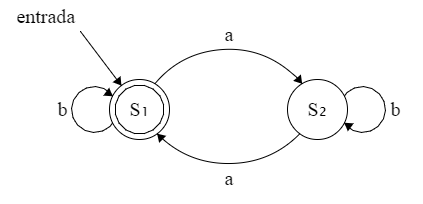
\includegraphics[scale=0.75]{aut01.png}
    \vspace{-0.5cm}
    \caption{Um autômato $M_1$.}
    \label{fig:aut01}
    \vspace{-0.5cm}
  \end{figure}


  No autômato da Figura~\ref{fig:aut01}, temos $Q = \{S_1, S_2\}$, $\Sigma = \{a, b\}$, $s = S_1$, $F = \{S_1\}$ e a função de transição  é dada pela tabela a seguir.
  \begin{table}[H]
    \centering
    \begin{tabular}[H]{c|c c}
      $\delta$ & \textbf{\texttt{a}} & \textbf{\texttt{b}} \\
      \hline
      $S_1$    & $S_2$               & $S_1$               \\
      $S_2$    & $S_1$               & $S_2$
    \end{tabular}
    \caption{Tabela de transições do $M_1$.}
    \label{tab:tabTransicoesM1}
    \vspace{-0.5cm}
  \end{table}


  Nesse exemplo, se o AFD $M_1$ é alimentado com a palavra \textbf{\texttt{aabab}}, ele irá começar no estado $S_1$ e irá percorrer os estados $S_2$, $S_1$, $S_1$, $S_2$, $S_2$ nesta ordem, e irá rejeitar a palavra dada (pois o último estado $S_2 \not\in F$). Se, para uma outra palavra $w$, a simulação tivesse terminado em $S_1$ (que pertence a $F$) diríamos que o autômato aceita a palavra $w$. Mais formalmente, se $M_1 = (Q, \Sigma, \delta, s, F)$ é um autômato finito determinístico, dizemos que $M_1$ \emph{aceita} $w$ se $\hat{\delta}(s, w) \in F$ e que $M_1$ \emph{rejeita} $w$ caso contrário.


  A \emph{linguagem reconhecida} por um autômato $M_1 = (Q, \Sigma, \delta, s, F)$ é o conjunto de palavras que são aceitas por esse autômato, ou seja, é definida pelo conjunto \[ L(M_1) = \{w \in \Sigma^* \colon \hat{\delta}(s, w) \in F \}.  \] No exemplo da Figura~\ref{fig:aut01} acima, a linguagem reconhecida por por $M_1$ é $L(M_1) = \{w \in \Sigma^* :  w \text{ tem número par de símbolos } \mathtt{a}\}$.
  % É comum estender a função de transição para uma função $\hat{\delta} \colon Q
  % \times \Sigma^* \rightarrow Q$ definida indutivamente por
  % \begin{enumerate}[(i)]
  % \item $\hat{\delta}(q, \sigma) = \delta(q, \sigma)$ para todo estado $q \in Q$ e símbolo $\sigma \in \Sigma$;
  % \item $\hat{\delta}(q, \sigma_1 \cdots \sigma_k) = \delta(\hat{\delta}(q, \sigma_1 \cdots \sigma_{k-1}), \sigma_k)$ para todo estado $q \in Q$ e símbolos $\sigma_1, \dots, \sigma_k \in \Sigma$.
  % \end{enumerate}
  \bigskip



  Vários tipos de exercícios pedem por uma resposta que é um autômato. Por exemplo:
  \begin{alineas}%[(i)]
    \item[(i)] construir um autômato que reconheça a linguagem regular
      dada por um certo conjunto de palavras descrito matematicamente;
    \item[(ii)] transformar um autômato finito não determinístico num
      determinístico equivalente;
    \item[(iii)] criar um autômato que reconheça a mesma linguagem
      descrita por uma expressão regular dada;
    \item[(iv)] construir o menor autômato finito determinístico
      que reconheça uma certa linguagem regular.
  \end{alineas}



  Cada um destes tipos de exercícios possui centenas de casos particulares que os alunos podem fazer para praticar os conceitos de autômatos abordados na disciplina. Tais exercícios podem, por exemplo, ser encontrados abundantemente no livro \textit{Introdução à Teoria da Computação} de M. Sipser~\cite{sipser}. Outras referências importantes da disciplina que possuem exercícios semelhantes são~\cite{ullman} e~\cite{linz}. Em todos os casos acima, contudo, há uma infinidade de respostas corretas para cada exercício. Por exemplo, considere o diagrama abaixo.

  \begin{figure}[H]
    \vspace{-0.5cm}
    \centering
    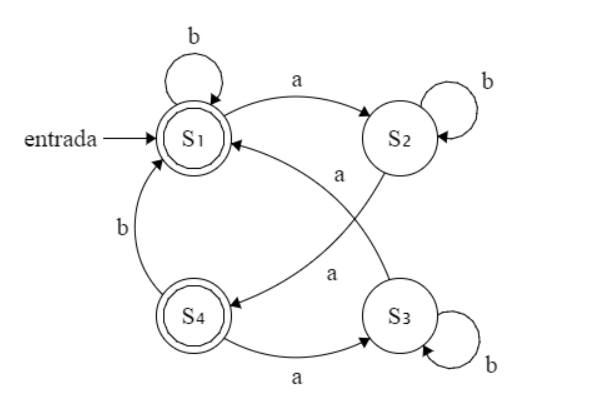
\includegraphics[scale=.65]{aut02.png}
    \vspace{-0.5cm}
    \caption{Um autômato $M_2$.}
    \label{fig:aut02}
    \vspace{-0.5cm}
  \end{figure}

  Apesar de visivelmente maior e mais complexo que $M_1$, este autômato reconhece a mesma linguagem que o autômato $M_1$ da Figura~\ref{fig:aut01}. É possível demonstrar que, para cada linguagem regular, existem infinitos autômatos que a reconhecem. Como decidir então se o autômato-resposta dado por um aluno reconhece a linguagem pedida? No caso do sistema que iremos desenvolver isso se reduz ao seguinte problema:
  \bigskip



  \noindent \textbf{Problema:} Decidir se dois autômatos finitos determinísticos reconhecem a mesma linguagem.

  %\newpage
\clearpage
\chapter[Métodos para resolver o problema da equivalência]{Métodos para resolver o problema da equivalência}

  Determinar se dois autômatos finitos e determinísticos reconhecem linguagens diferentes é um problema bem resolvido. A ideia fundamental é tentar encontrar uma palavra $w$ que é aceita por um autômato e rejeitada pelo outro. Se tal palavra puder ser encontrada, então as linguagens reconhecidas por esses autômatos são distintas. Caso tal palavra não exista, os autômatos reconhecem a mesma linguagem.



  Mais formalmente, dizemos que dois estados $q_1$ e $q_2$ (no mesmo autômato ou não) são \emph{equivalentes} se, para toda palavra $w \in \Sigma^*$ vale que $\hat{\delta}(q_1, w) \in F$ se e somente se $\hat{\delta}(q_2, w) \in F$, caso contrário $q_1$ e $q_2$ sao  chamados distinguíveis. Dois autômatos serão, portanto, equivalentes  se e somente se seus respectivos estados iniciais forem equivalentes  no sentido que acabamos de definir.



  Esse problema está intimamente relacionado com o problema de minimização de autômatos finitos determinísticos. Os primeiros algoritmos desenvolvidos para testar a equivalência de autômatos resolviam também o problema da minimização. Eles apareceram em~\cite{huffman} e~\cite{moore} e podem ser implementados sem muito esforço em tempo $O(n^4)$, onde $n$ é o número total de estados. O algoritmo mais eficiente conhecido para minimização de autômatos~\cite{hopcroft} executa em tempo $O(n \log{}n)$. Posteriormente Hopcroft e Karp~\cite{hopcroft_karp} desenvolveram um algoritmo linear para testar a equivalência de autômatos.



\section{Minimização de Moore}
  %[ULLMAN pag. 154 – 4.4 Equivalence and Minimization of Automata (pdf 168)]

  Nessa seção vamos investigar um algoritmo de minimização de autômato finito determinístico, mais especificamente o algoritmo de Minimização de Moore~\cite{moore} e discultido no~\cite{ullman}.

  Para facilitar a compreensão utilizaremos como exemplo o autômato $M_2$ da Figura~\ref{fig:aut02}. Queremos determinar se $M_2$ é equivalente ao autômato $M_1$ da Figura~\ref{fig:aut01}.

  O autômato $M_2$ é representado pela quíntupla $M_2 = (Q, \Sigma, \delta, s, F)$, onde temos $Q = \{S_1, S_2, S_3, S_4\}$, $\Sigma = \{a, b\}$, $s = S_1$, $F = \{S_1, S_4\}$ e a função de transição é dada pela tabela a seguir.

  %__|__a__b_
  %S1| S2 S1
  %S2| S4 S2
  %S3| S1 S3
  %S4| S3 S1
  \begin{table}[H]
    \centering
    \begin{tabular}[H]{c|c c}
      $\delta$ & \textbf{\texttt{a}} & \textbf{\texttt{b}}\\
      \hline
      $S_1$    & $S_2$               & $S_1$              \\
      $S_2$    & $S_4$               & $S_2$              \\
      $S_3$    & $S_1$               & $S_3$              \\
      $S_4$    & $S_3$               & $S_1$              \\
    \end{tabular}
    \caption{Tabela de transição do $M_2$.}
    \vspace{-0.5cm}
  \end{table}

  Note que a definição de estados equivalentes na seção anterior não se traduz imediatamente em um algoritmo, pois não é possível testar se $\hat{\delta}(p, w) \in F$ para todas as palavras $w \in \Sigma^*$

  No entanto, podemos desenvolver um algoritmo para determinar a equivalência entre estados $p$ e $q$ baseando-se no seguinte lema:

  \newtheorem{lemma}{Lema}
  \begin{lemma}
    \label{lemma01}
    Se $r = \delta(q,\sigma)$ e $s = \delta(p,\sigma)$ e se $r$ e $s$ são  distinguíveis, então $p$ e $q$ são distinguíveis.
  \end{lemma}

  %\noindent\textbf{\textit{Base.}} Se $p$ é um estado de aceitação e $q$ é um estado de não aceitação, então o par $\{p,q\}$ é distinguível.

  \begin{proof}[\textbf{Prova}]
    %Temos os estados $p$ e $q$ que ao entrar com o simbolo $\sigma$, teremos $r = \delta(q,\sigma)$ e $s = \delta(p,\sigma)$ na qual sabemos que $r$ e $s$ são distinguíveis. Então o par $p$ e $q$ também é distinguível, pois para este lema faça sentido
    Por hipótese deve haver uma palavra $w$ que distingue $r$ de $s$, ou seja, exatamente um dos estados $\hat{\delta}(r, w)$ e $\hat{\delta}(s, w)$ é de aceitação. Então a palavra $\sigma w$ distingui $p$ de $q$, já que $\{\hat{\delta}(p, \sigma w), \hat{\delta}(q, \sigma w)\}$ é o mesmo par de estados que $\{\hat{\delta}(r, w), \hat{\delta}(s, w)\}$.
  \end{proof}

%  \textcolor{blue}{\textbf{[LIVRO ULLMAN pag 155]}}\\

  %\textcolor{blue}{\textbf{FALAR DO PROCESSO}} ( O lema 1 é só um principio que norteia o processo )

  A partir do Lema acima podemos elaborar um processo para investigar quais são os pares de estados que são distinguíveis. Para qualquer par de estados, eles são distinguíveis se constatar que um simbolo do alfabeto aplicado na função $\delta$, em cada estado deste par, resulta em um par de estados que já estão distinguidos. E também ter como premissa que se num par de estados, um destes estados é de aceitação e o outro não, então estes estados são distinguidos com a palavra vazia, denotada por $\varepsilon$.

  Entendido o processo de como verificar se um par de estados são distinguíveis, podemos ver o pseudo código, que realiza as verificações para todos os possíveis pares, logo a baixo.\\


  \vspace{-0.5cm}
  \begin{algorithm}[H]
    \label{alg01}
    \caption{Acha Pares Distinguíveis pela Minimização de Moore}
    \Entrada{$Q, \Sigma, \delta, F$}
    \Saida{Tabela de distinguibilidade }
    \Inicio{
      \ParaCada{ $p \in Q$ }{
        \ParaCada{ $q \in Q$ }{
        $D\{p,q\} \gets \emptyset$
        }
      }
      \ParaCada{ $p \in F$ }{
        \ParaCada{ $q \in Q \backslash F$ }{
        $D\{p,q\} \gets$ x
        }
      }
      distinguiu{\_}algo $\gets$ verdadeiro\\
      \Enqto{distinguiu{\_}algo}{
        distinguiu{\_}algo $\gets$ falso\\
        \ParaCada{ $p \in Q$ }{
          \ParaCada{ $q \in Q$ }{
            \Se{$D\{p,q\} = \emptyset$}{
              \ParaCada{ $\sigma \in \Sigma$ }{
                \Se{$D\{\delta(p,\sigma), \delta(q, \sigma)\} \neq \emptyset$}{
                  $D\{p,q\} \gets$ x \\     %\sigma $\\
                  distinguiu{\_}algo $\leftarrow$ verdadeiro\\
                }
              }
            }
          }
        }
      }
      \Retorna{D}
    }
  \end{algorithm}

  Ao analisarmos este pseudo código de algoritmo de minimização vemos que este recebe como entrada o conjunto de estados $Q$, o alfabeto $\Sigma$, a tabela de transição $\delta$ e o conjunto de estados finais $F$ de um autômato.

  E contamos com o apoio de uma matriz quadrada simétrica $D$ de dimensão $|Q|\times|Q|$, cujas células abaixo da diagonal principal serão utilizadas para representar todos os pares de estados possíveis. Inicialmente, $D$ será inicializada com valores vazios. Ao longo da execução do algoritmo, se um par for distinguido, então atribuiremos o simbolo “x” à célula correspondente a este par. Logo em seguida, preenchemos as células dos pares trivialmente distinguíveis, ou seja, pares que consistem de um estado final e um não final.

  Então iniciam-se as rodadas de verificação, onde percorre-se $D$ e para cada par $\{p, q\}$ com valor vazio, o algoritmo testa para cada carácter $\sigma$ do conjunto $\Sigma$, se o par $\{p, q\}$ se torna distinguível pelo caractere $\sigma$, considerando $\hat{\delta}(p, w)$ e $\hat{\delta}(q, w)$ em vista do Lema~\ref{lemma01}.

  Além disto, com o apoio da variável booleana $distinguiu{\_}algo$, utilizada para marcar se houve uma alteração em $D$, verificamos que as rodadas somente cessarão se, na mesma rodada, nenhum ``x'' é adicionado na tabela de distinguibilidade, concluindo assim que não existem mais pares à ser distinguídos. Retornando, ao fim, a tabela de distinguibilidade.

  Concluímos que não pode haver mais de $O(n^2)$ verificações em uma rodada, assim certamente o limite superior para o número de verificações é $O(n^4)$, visto que o pior caso é atingido quando somente um único par de estados é distinguido por rodada, causando $O(n^2)$ rodadas com $O(n^2)$ verificações em cada, onde $n$ é o tamanho do conjunto~$Q$.

  Então, para solucionamos o nosso problema de verificar se dois autômatos são equivalentes, podemos considerar um terceiro autômato que é a união disjunta dos dois autômatos dados e executamos o algoritmo acima sobre a união. E, ao final, apenas verificamos se a posição na tabela que representa o par de estados iniciais encontra-se vazia.

  %se os estados iniciais dos dois autômatos se encontram equivalente na tabela de distinguibilidade retornada pelo método.

  Para o nosso exemplo, ao unirmos o $M_1$ com o $M_2$, obtemos a seguinte tabela de transição. Mas com a nomenclatura dos estados de $M_2$ mapeados de $\{S_1, S_2, S_3, S_4\}$ para $\{S_3, S_4, S_5, S_6\}$.

  % _|_a_b
  % 1| 2 1
  % 2| 1 2
  % 3| 4 3
  % 4| 6 4
  % 5| 3 5
  % 6| 5 3
  \begin{table}[H]
    \centering
    \begin{tabular}[H]{c|c c}
      $\delta$ & \textbf{\texttt{a}} & \textbf{\texttt{b}} \\
      \hline
      $S_1$    & $S_2$               & $S_1$               \\
      $S_2$    & $S_1$               & $S_2$               \\
      $S_3$    & $S_4$               & $S_3$               \\
      $S_4$    & $S_6$               & $S_4$               \\
      $S_5$    & $S_3$               & $S_5$               \\
      $S_6$    & $S_5$               & $S_3$               \\
    \end{tabular}
    \caption{Tabela de Transição dos autômatos $M_1$ e $M_2$ unidos.}
    \vspace{-0.5cm}
  \end{table}

  E ao executar o algoritmos de equivalência, obteremos a seguinte tabela de distinguibilidade.

  %2| #
  %3| -  #
  %4| #  -  #
  %5| #  -  #  -
  %6|_-__#__-__#__#_
  %   1  2  3  4  5
  \begin{table}[H]
    \centering
    \begin{tabular}{c c c c c c}
      \cline{2-2}
      $S_2$ & \multicolumn{1}{|c|}{x}  \\
      \cline{2-3}
      $S_3$ & \multicolumn{1}{|c|}{ } & \multicolumn{1}{c|}{x}  \\
      \cline{2-4}
      $S_4$ & \multicolumn{1}{|c|}{x} & \multicolumn{1}{c|}{ } & \multicolumn{1}{c|}{x} \\
      \cline{2-5}
      $S_5$ & \multicolumn{1}{|c|}{x} & \multicolumn{1}{c|}{ } & \multicolumn{1}{c|}{x}  & \multicolumn{1}{c|}{ } \\
      \cline{2-6}
      $S_6$ & \multicolumn{1}{|c|}{ } & \multicolumn{1}{c|}{x} & \multicolumn{1}{c|}{ } & \multicolumn{1}{c|}{x} & \multicolumn{1}{c|}{x} \\
      \cline{2-6}
          & $S_1$                   & $S_2$                  & $S_3$                  & $S_4$                  & $S_5$                  \\
    \end{tabular}
    \caption{Tabela de distinguibilidade dos autômatos $M_1$ e $M_2$ unidos.}
    \vspace{-0.5cm}
  \end{table}


  Basta agora verificar se a posição da matriz $D$ correspondente ao par de estados iniciais está com o seu valor vazio, o que indica que os estados iniciais são equivalentes. Neste caso, os autômatos $M_1$ e $M_2$ são equivalentes.


%\subsection {Detalhes de Implementação do Algoritmo de Minimização}
%  Como visto na seção anterior, o que faz o Algoritmo~\ref{alg01} estar sobrecarregado é o fato de que, em todas as rodadas, ele procura pelo próximo par de estados que ainda não foi distinguido, que é feito pelas linhas 11, 12 e 13 do pseudo-código anterior. Assim, uma solução possível para melhorar a eficiência do algoritmo seria manter informações extras na memória de modo que, ao realizar uma verificação da distinguibilidade de um par, ele já deve ter conhecimento de qual é o próximo par à ser checado.
%
%  Intuitivamente, se faz necessário o uso de uma estrutura de dados para abrigar os índices das células desta matriz $D$, que representam um par. E esta estrutura de dados terá como regra de inserção e remoção de elementos no formato de que o primeiro a entrar será o primeiro a sair, ou seja, uma fila. Então todos os elementos que estiverem contidos nesta fila, obrigatoriamente ainda não foram distinguidos.
%
%  Temos então que fazer algumas alterações no código do Algoritmo~\ref{alg01}. Anteriormente à linha 9, em que se dá o inicio das rodadas de verificação, devemos inserir na fila todos os pares que não foram trivialmente distintos e ao final adicionamos um elemento chave, que tem a função de marcar o final de uma rodada.
%
%  A seguir inicia-se as rodadas de verificação, em que será removido um a um os elementos da fila e verificamos primeiramente se este elemento se trata do elemento chave. Se sim, com o auxilio da variável booleana $distinguiu{\_}algo$, verificaremos se foi distinguido algum par de estados durante a rodada. Se não houve um novo par distinguido, então encerra-se as rodadas, caso contrario inserimos o elemento chave de volta a fila.
%
%  Mas caso não seja o elemento chave, tentamos verificar se o par que este elemento representa pode ser distinguido para todas os símbolos de $\Sigma$ conforme o Lema~\ref{lemma01}. E se aquele par for distinguível, marcamos a celula de $D$ como distinguido. Se e somente se o par não for distinguido, ele será novamente inserido na fila, para que na próxima rodada o  torne a verificar.
%
%  Assim ao final das rodadas de verificação, os elementos contido na fila serão os representantes dos pares indistinguíveis.
%
%  Com esta estratégia, conseguiremos eliminar as verificações dos pares que já foram distinguidos durante as rodadas que o algoritmo executa. Utilizando mais memória para armazenar esta estrutura de dado que auxilia na verificação, mas proporcionando uma melhora significativa no desempenho do Algoritmo~\ref{alg01}.



\subsection {Recuperação de Palavra}

  Este sistema de apoio a aprendizagem tem como objetivo o rápido feedback sobre a resposta submetida pelo usuário. Com a ajuda do Algoritmo~\ref{alg01} conseguimos verificar se o autômato-resposta é equivalente ao autômato-gabarito perfeitamente. Mas, caso o Algoritmo~\ref{alg01} retornar que não são equivalentes, então se faz necessário de uma dica ao usuário para que ele tome conhecimento de seu erro. Esta dica será uma palavra $w \in \Sigma^*$, que distingue o estado inicial do autômato-resposta submetido do estado inicial do autômato-gabarito, e ao ser percorrida pelo usuário, permite encontrar o erro cometido em sua resposta.

  Então é necessária a implementação de um algoritmo que descubra qual é essa palavra que distingue os dois autômatos. Para que seja possível encontrar a palavra desejada é necessário modificar o Algoritmo~\ref{alg01}, para que ele não somente descubra quais pares de estados são distinguíveis, mas também guarde os símbolos iniciais das palavras que as distinguem. Isso pode ser feiro alterando-se apenas as linhas 7 e 16 do Algoritmo~\ref{alg01} como indicado a seguir:

  \begin{alineas}%[(i)]
    \item[7.]  $ D\{p,q\} \gets \varepsilon $
    \item[16.] $ D\{p,q\} \gets \sigma $
  \end{alineas}

  %Previamente temos que fazer uma alteração na matriz $D$, em que ao invés de receber o simbolo “x”, atribuiremos agora o simbolo $\sigma \in \Sigma$ que os distinguiu, mais especificamente na linha 7 e 16 do Algoritmo~\ref{alg01}.

  Então supondo que $D\{p,q\} \neq \emptyset$, temos o seguinte  pseudo código.

  \begin{algorithm}[H]
    \caption{Acha a palavra que distingui os dois autômatos}
    \label{alg02}
    \Entrada{$ D, \delta, \{p_0, q_0\}$}
    \Saida{ w }
    \Inicio{
      $ w \gets \varepsilon $\\
      $ \{p, q\} \gets \{p_0, q_0\} $ \\
      $ \sigma \gets D(\{p, q\}) $\\
      \Enqto{$\sigma \neq \varepsilon$} {
        $ w \gets w \cdot \sigma $\\
        $ \{p, q\} \gets \{\delta(p, \sigma), \delta(q, \sigma)\} $\\
        $ \sigma \gets D(\{p, q\}) $
      }
      \Retorna{ w }
    }
  \end{algorithm}

  O algoritmo recebe como entrada $D$, $\delta$ e $\{p_0, q_0\}$, que é a tabela de distinguibilidade gerado pelo Algoritmo~\ref{alg01} com as modificações sugeridas acima, a tabela de transição dos autômatos unidos e o par de estados iniciais dos autômatos, respectivamente.

  O Algoritmo~\ref{alg02} irá coletando os símbolos contidos em células especificas de $D$ e unindo-os ao conjunto $w$. Inciando pelo par $\{p_0, q_0\}$, descobrindo o simbolo que os distinguem e atribuindo a $\sigma$. E enquanto não encontrar o simbolo $\sigma$ com o valor $\varepsilon$, unirá ao conjunto $w$ o simbolo $\sigma$, em seguida descobre o próximo par de estados que o simbolo $\sigma$ levará utilizando a tabela de transição, ou seja, o novo par será $\{\delta(p, \sigma), \delta(q, \sigma)\}$, e por ultimo descobre qual é o simbolo que distinguiu este próximo par de estados.

   %Para finalizar, faz uma ultima verificação se o conjunto $palavra$ esta vazio, se caso positivo então incluímos o simbolo $\varepsilon$ em $palavra$.

  Então será retornado o a palavra $w$, que é a palavra que distinguiu os dois autômatos que estávamos procurando.






  %\newpage
\section {Equivalência em Tempo Linear}

  A maioria dos algoritmos para teste de equivalência de autômatos finitos determinísticos na literatura tem crescimento assintótico proporcional ao quadrado do número de estados~\cite{ullman}. Um algoritmo desenvolvido por Hopcroft e Karp~\cite{hoka71}, para este mesmo fim, tem complexidade de $O(n \log{}^* n)$, onde $n$ é o número de estados. Nesta seção estudaremos este algoritmo. %Então estudaremos este algoritmo nesta seção.

  Mas antes temos que entender a estrutura de dados utilizada para armazenar conjuntos disjuntos, conhecida popularmente como \textit{Union-Find}, que será fundamental para o método de equivalência de Hopcroft e Karp.


\subsection {A Estrutura Union-Find}

  Para o método que veremos na seção seguinte, envolve o agrupamento de elementos em uma coleção de conjuntos disjuntos\footnote{São quando os conjuntos não tem elementos em comum, ou seja, suas interseções é o conjunto vazio.}, e há uma estrutura de dados que atende este requisito~\cite{cormen} e admite duas operações que será vital para a implementação do algoritmo de equivalência em tempo linear. %\footnote{Conjuntos disjuntos são quando a cada dois conjuntos, a sua interseção é o conjunto vazio.}

  %A primeira operação é o FIND, que basicamente tem a função de dado um elemento no parâmetro, encontrar a qual conjunto este elemento pertence. A segunda operação é o MERGE, que tem a função de fundir os dois conjuntos em um. Adiante iremos aprofundar melhor em seus detalhes.~\cite{cormen}

  Na estrutura de dados de conjuntos disjuntos guarda-se um coleção de elementos disjuntos. Onde cada conjunto é identificado por um representante, que será um de seus elementos, não importando na maioria dos casos qual seja este elemento, somente que será sempre ele que atenderá quando for procurado o representante daquele conjunto.

  Para se criar um conjunto utiliza-se a função \texttt{MAKE-SET($x$)}, que aloca um conjunto contendo um elemento $x$ na memória, este elemento será o representante deste conjunto, e claro $x$ não deverá estar presente em nenhum outro conjunto.

  A operação \texttt{FIND($x$)} basicamente tem a função de dado um elemento $x$, encontrar a qual conjunto este elemento pertence, retornando o seu elemento representante.

  A outra operação é o \texttt{MERGE($x$, $y$)}, que tem a função de fundir os dois conjuntos que os elementos $x$ e $y$ pertencem em somente um na coleção.

  Há mais de um modo de implementar esta estrutura, usando listas ligadas ou até lista de árvores, por exemplo.

  Com a lista ligada, temos o primeiro elemento de cada lista sendo o representante, e cada objeto desta lista tem um ponteiro para o próximo objeto e um ponteiro direto para o representante. Deste modo facilita a operação \texttt{FIND} por ter um ponteiro direto para o representante. Mas para o \texttt{MERGE}, não basta somente o ultimo objeto do primeiro conjunto apontar para o inicio do segundo conjunto, há a necessidade de atualizar o ponteiro para o novo representante de todos os elementos do segundo conjunto. Causando um aumento na complexidade do algoritmo.

  Já se utilizarmos uma estrutura de árvore, em que cada elemento será um objeto  que representa um nó na árvore. Então este nó somente basta ter um ponteiro para seu nó pai, e o representante será aquele que apontar para ele mesmo. A operação \texttt{MERGE} se torna mais simples, mas o ponteiro da raiz do segundo apontar para a raiz do primeiro conjunto. Já o \texttt{FIND} terá que percorrer a partir do pais deste elemento, todos os pais de seus ancestrais, até encontrar a raiz, que é o representante deste conjunto. Isso pode se tornar custoso caso a altura da árvore seja muito grande, por isso uma otimização da estrutura se faz necessária, utilizando um método de compactação do caminho até a raiz.

  Cada implementação tem a sua particularidade e a escolha depende de seu uso, para o Algoritmo de Hopcroft e Karp, será implementada como modo de árvores, que discutiremos e analisaremos melhor nas seções seguintes.

  Para ilustrar melhor esta estrutura, temos o seguinte exemplo:

  \begin{alineas}
  \item[$\bullet$]
    Criamos uma coleção de conjuntos disjuntos $\Psi  = \{S_1, S_2, S_3, S_4, S_5\}$, onde para cada conjunto $S_i$ temos o elemento $i$ contido nele e este será o representante do conjunto disjunto. Criando $\{ \{\underline{1}\}, \{\underline{2}\}, \{\underline{3}\}, \{\underline{4}\}, \{\underline{5}\}\}$. Os elementos sublinhados caracteriza o representantes daquele conjunto.
    \begin{figure}[!ht]
      \centering
      \vspace{-0.3cm}
      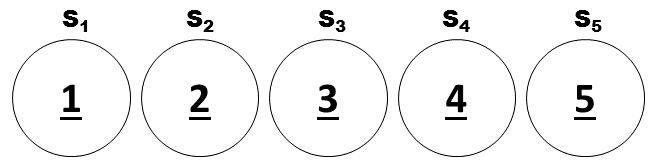
\includegraphics[scale=0.4]{unionFind_exemplo1.png}
      \vspace{-0.5cm}
    \end{figure}

  \item[$\bullet$]
    \texttt{MERGE(2, 3)} resulta em $\{ \{\underline{1}\}, \{2, \underline{3}\}, \{\underline{4}\}, \{\underline{5}\}\}$.
    \begin{figure}[H]
      \centering
      \vspace{-0.3cm}
      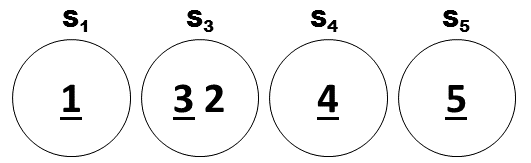
\includegraphics[scale=0.4]{unionFind_exemplo2.png}
      \vspace{-0.5cm}
    \end{figure}


  \item[$\bullet$]
    \texttt{MERGE(5, 4)} resultado em $\{ \{\underline{1}\}, \{2, \underline{3}\}, \{\underline{4}, 5\}\}$.
    \begin{figure}[H]
      \centering
      \vspace{-0.3cm}
      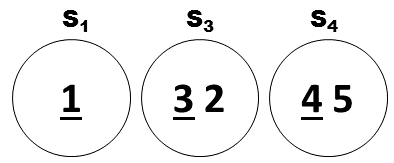
\includegraphics[scale=0.4]{unionFind_exemplo3.png}
      \vspace{-0.5cm}
    \end{figure}

  \item[$\bullet$]
    \texttt{FIND(2)} será retornado o elemento \texttt{3}.

  \item[$\bullet$]
    \texttt{FIND(3)} será retornado o elemento \texttt{3}.
  \end{alineas}




\subsection {Algoritmo de Hopcroft e Karp}

  Nesta seção estudaremos o algoritmo de Hopcroft e Karp para o teste de equivalência em tempo linear~\cite{hoka71}. O algoritmo utilizas-se da estrutura de dados pilha e uma estrutura de dados popularizada como Union-Find para armazenar conjuntos disjuntos~\cite{cormen}. Em especial esta última estrutura de dados tem fundamental importância no algoritmo para testar a equivalência dos autômatos, pois armazenará no mesmo conjunto os estados que são equivalentes.

  Vejamos a seguir o algoritmo.

  \begin{algorithm}[H]
    \caption{Teste de Equivalência de Hopcroft e Karp}
    \label{alg03}
    \Entrada{$ Q, \delta, \{p_0, q_0\}$}
    \Saida{ Conjuntos disjuntos }
    \Inicio{
      conjuntos.INIT($|Q|$) \\
		  conjuntos.MERGE($p_0, q_0$) \\
		  pilha.empilha($\{p_0, q_0\}$) \\
		  \Enqto{pilha $\neq \emptyset$} {
		    $\{p, q\} \gets$ pilha.desempilha() \\
		    \ParaCada{$\sigma \in \Sigma$} {
		      $r \gets$ conjuntos.FIND( $\delta(p, \sigma)$ ) \\
		      $s \gets$ conjuntos.FIND( $\delta(q, \sigma)$ ) \\
		      \Se{$r \neq s$} {
		        conjuntos.MERGE($r, s$) \\
		        pilha.empilha($\{r, s\}$) \\
		      }
		    }
		  }
		  \Retorna{conjuntos}
		}
  \end{algorithm}


  A estrutura de dados Union-Find armazena conjuntos disjuntos na memória, e deseja-se executar essencialmente duas operações: MERGE($i, j$), une o conjunto $i$ ao conjunto $j$, e FIND($i$) busca o conjunto ao qual pertence o elemento $i$.

  O algoritmo inicia-se criando a estrutura de dados Union-Find, que atribuímos o nome de $conjuntos$, e terá o tamanho igual ao tamanho do conjunto $Q$, que é novamente a união dos dois autômatos que queremos testar sua equivalência. Assim a estrutura conterá $|Q|$ conjuntos e em cada um contendo um único elemento que corresponde a um estado de $Q$, e cada conjunto é denominado pelo nome do elemento que é o representante daquele conjunto. Ou seja, cada estado de $Q$ está em seu próprio conjunto, sendo ele mesmo o representante e nome deste conjunto.

  Realizaremos a primeira fusão, entre os conjunto $p_0$ e $q_0$, pois supomos que se os autômatos são equivalentes, então seus estados iniciais também deverão ser equivalentes. EM seguida utilizaremos uma estrutura de dados de Pilha para armazenar o par destes dois estado iniciais.

  Assim inicia-se as verificações até que esta pilha esteja vazia. Primeiro desempilhamos um par da pilha e atribuímos a variáveis $\{p,q\}$. Então para cada simbolo $\sigma$ do alfabeto $\Sigma$ será feito algumas etapas. Buscamos qual é o conjunto que contém o estado que foi levado pela função de transição $\delta$ ao entrar com o simbolo $\sigma$ e denominaremos estes de $r$ e $s$. E verificaremos se $r \neq s$, ou seja, se o conjunto $r$ é diferente do conjunto $s$. Se sim, então uniremos estes dois conjuntos e empilhamos o par $\{r, s\}$ na pilha.

  Assim o algoritmo somete terminará ao analisar todos os estados para todas as letras do alfabeto, retornando ao final o $conjuntos$.

  Então para constatar a equivalência, basta examinar em cada conjunto $q$ da lista de conjuntos disjuntos se $q \subset F$ ou $q \subset Q \backslash F$. Ou seja, os dois autômatos são equivalentes se, e somente se em nenhum conjunto da lista há estados de aceitação e de não aceitação no mesmo conjunto.

  Os passos das linhas 2, 3, 4 e a verificação final desta lista, são executadas em uma quantidade limitada por uma constante de tempo $n$, onde $n$ é o número de estados de $Q$.

 Já o tempo de execução da interações da linha 5 até a 12, tem o tempo limitado pelo número de vezes que os pares são removidos da pilha. Que por sua vez, o número de pares retirados da pilha é limitado por $n$, pois cada vez que um par é inserido na pilha, dois conjuntos são fundidos, assim o número total de conjuntos é diminuído em um. Desde a inicialização, são definidos $n$ conjuntos e no máximo $n-1$ pares são colocados na pilha.

 Então o tempo de execução deste algoritmo para testar a equivalência de dois autômatos finitos é delimitados por uma constante vezes o produto do tamanho do alfabeto pelo o número de estados, ou seja, $O(c \times |\Sigma| \times |Q|)$.

 Mas como utilizamos a estrutura de dados Union-Find temos o consumo de tempo limitados superiormente por $O(n \log^* n)$.
 %A função FIND tem em si uma otimização da estrutura, que acarreta em um tempo de $O(\log n)$ no pior caso, e esta função dentro do Algoritmo~\ref{alg03} é executada $n$ vezes, assim faz o algoritmo ser limitado superiormente por $O(n \log n)$. Veremos mais detalhes desta estrutura na seção seguinte.



\subsection {Detalhes de Implementação do Algoritmo de Teste de Equivalência} %{Detalhes de Implementação do Algoritmo de Teste de Equivalência de Hopcroft e Karp }

  O algoritmo utiliza-se de duas estruturas de dados, uma pilha para armazenar o próximo par a ser analisado e o Union-Find para armazenar conjuntos disjuntos.

  A pilha utilizada na implementação é a oferecida pela biblioteca padrão da linguagem. Já o conjunto disjunto pode ser simplificada, pois sua utilização neste algoritmo, a estrutura de dados não necessita ter alocação de memória dinâmica. Logo, para sua implementação basta a alocação de um único vetor sequencial de tamanho igual ao passado por parâmetro no método INIT. Para isto, os atributos padrão destra estrutura de dados serão simplificados, provendo assim uma economia de memória.

  Cada índice deste vetor, representará um elemento a ser agrupado em conjuntos, que por sua vez representa um estado da união dos dois autômatos. O valor daquele elemento no vetor representará o seu pai. E quando este valor apontar para si mesmo, significa que este elemento é o elemento raiz, também chamados de representante do conjunto que ele está contido. O atributo \textit{rank} não se fará necessário para esta implementação simplificada. Esta estrutura se assemelhará a uma árvore, em que cada elemento há somente o ponteiro para seu pai.

  Assim com esta estrutura, podemos implementar somente os métodos necessários para manipular os conjuntos disjuntos que o algoritmo necessita.

  Os passos para a implementação da função MERGE serão as seguintes: recebido dois índices por parâmetro, buscamos os conjuntos que os contêm com auxilio da função FIND e por fim fazemos o primeiro conjunto ser subconjunto do segundo, ou seja, a raiz do primeiro terá seu valor apontando para a raiz do segundo conjunto.

  Já o método FIND, recebe um elemento por parâmetro, e retorna o índice do elemento raiz (o representante) do conjunto que contem o elemento passado como parâmetro.

%  Já o método FIND, recebe um elemento por parâmetro, e verificar se ele é a raiz, ou seja, se o valor aponta para ele mesmo, se sim este é a raiz e nome do conjunto, e retornando-o. Se não, haverá uma busca em profundidade em seu parente recursivamente, ao encontra a raiz, será devolvida seu valor e atribuído este valor ao valor do elemento. Forçando assim que o elemento e todos seus parentes até atingir a raiz agora apontam diretamente para a raiz. Esta otimização da estrutura garante uma compactação do caminho até a raiz.

  Para testar a equivalência de dois autômatos, inicialmente supomos que eles são equivalentes, logo os seus estados iniciais são equivalentes. Por conta disto acontece a primeira chamada do método MERGE para o par $\{p_0, q_0\}$ correspondente ao par de estados inciais dos dois autômatos. E assim inicia-se as verificações até que não haja mais conjuntos a serem unidos.

  Há ainda a possibilidade de otimizar este código, pois ao final da execução do algoritmo, temos que verificar todos os conjuntos resultantes da estrutura de dados Union-Find. Se durante a execução do Algoritmo~\ref{alg03} for haver uma união de conjuntos, basta verificarmos cada um dos representantes se um é estado de aceitação e o outro não. Então comprovando que aqueles dois autômatos não são equivalentes, não necessitando terminar todas as interações para verificar todos os conjuntos somente ao final. Então se encontrado uma união heterogênea, o algoritmo deve cessar. E acontecerá esta verificação anteriormente as linhas 3 e 11 do Algoritmo~\ref{alg03} nos conjuntos que pretendem ser unidos.

  %Mas se fizermos a verificação antes da chamada do método MERGE, nas linas 3 e 11, se os dois conjuntos pretendentes a união são heterogêneo a respeito de serem todos estados de aceitação ou não, podemos terminar a execução ali mesmo, pois já resultaria que os dois autômatos não são equivalentes.



\subsection {Recuperação de Palavra}

  Para poder encontrar uma palavra que demonstre a distinção dos dois autômatos, a partir da otimização proposta na seção anterior, facilmente percebemos que, se o algoritmo for terminado por tentar unir dois conjuntos heterogêneos, então exite uma palavra que os distingue. Basta agora recuperar esta palavra, e para isto temos que recuperar todas as uniões que foram efetuadas até o momento do término.

  %Sabemos que se houve uma união de conjuntos, então houve a insertação do próximo par na pilha.
  Uma possível solução, que foi implementada, é que a cada união de conjuntos devemos guardar em uma nova pilha as informações a respeito desta união. Então armazenamos a tupla $\{p, q, \sigma, r, s\}$, que basicamente são as variáveis daquela interação, onde $p$ e $q$ é o par que estava sendo verificado pelo simbolo $\sigma$, que causou a união do par $r$ e $s$.
  %que anteriormente a verificação, se é possível a união, inserimos um par nesta pilha histórico e anexo a ele, qual foi o par anterior e qual o simbolo que possibilitou a união dos conjuntos. Ou seja, inserimos o conjunto $\{p, q, r, s, \sigma\}$.

  Então no Algoritmo~\ref{alg03}, basta acrescentar a instrução de empilhar esta tupla na pilha, que chamaremos de \emph{pHist}, após as linhas: 3 e 11.

  No pseudo código a seguir veremos a implementação da recuperação desta palavra.

  \begin{algorithm}[H]
    \caption{Recuperação da palavra que os distinguem}
    \label{alg04}
    \Entrada{$ pHist $}
    \Saida{ $ w $ }
    \Inicio{
      $w \gets \varepsilon $ \\
      \Enqto{$pHist \neq \emptyset$}{
        $\{p, q, \sigma, r, s\} \gets $pHist.desempilha() \\
        $w \gets \sigma \cdot w$ \\
        \Enqto{$(pHist.topo().r \neq p) ~ | ~ (pHist.topo().s \neq q)$}{  %(pHist \neq \emptyset) ~\&~
          pHist.desempilha() \\
        }
      }

		  \Retorna{w}
		}
  \end{algorithm}


  Assim teremos uma pilha com o histórico das uniões. Então se o Algoritmo~\ref{alg03} terminou por ter encontrado uma união não desejada, basta agora ir retirando os elementos desta pilha histórico até esvaziar, adicionando à variável $w$ o simbolo que causou a união. E por fim encontrar o par de estados que uniu este par sucessor, dispensando os elementos que não estamos procuramos.

  Poderíamos abstrair melhor este algoritmo como se a cada verificação a partir da raiz ($\{p_0, q_0\}$) no Algoritmo~\ref{alg03} fosse uma busca em profundidade, que se interrompida em algum ponto, então o caminho de volta até a raiz a partir deste ponto, recolhendo os símbolos associada a cada união, forma a palavra que distinguiu os dois autômatos.
%a recuperação da palavra seria um

\section{Escolha do Melhor Método}
  Após implementar e analisar cada algoritmo que discutimos até aqui, devemos escolher qual deles deve ser incluído no sistema. Ambos cumprem a tarefa de verificar a equivalência entre dois autômatos, e ambos são capazes de recuperar a palavra que diferencia um autômato do outro, no caso de eles não serem equivalentes.

  Claramente o algoritmo de teste de equivalência de Hopcroft e Karp se destaca comparado ao método de minimização de Moore, pelo fato dele ter complexidade linear, o que possibilita atingir um maior desempenho, que é uma característica desejável para o sistema.






 \chapter[O sistema] {O sistema}
  %Não podemos negar que a internet está difundida na sociedade: ela está em todos os lugares, tanto em computadores como em televisores e em celulares.
  A plataforma que desenvolvemos possibilita uma experiência de uso semelhante ao de um aplicativo para \textit{desktop}, mas não necessita de instaladores e não depende de um sistema operacional especifico como os programas tradicionais.

  Uma aplicação web é um sistema que possibilita a intercomunicação entre um cliente e um servidor via internet. O cliente é um navegador, que exibe uma interface gráfica e proporciona uma interação com o usuário. Já o processamento fica ao encargo de um servidor HTTP\footnote{Abreviação para \textit{Hypertext Transfer Protocol}, em português Protocolo de Transferência de Hipertexto, é um protocolo base para a comunicação de dados da \textit{World Wide Web}.}. Este servidor tem a função de receber requisições e devolver respostas ao cliente. E o cliente exibe as informações ao usuário e solicita recursos a este servidor conforme o usuário interage com o navegador.

  Assim este sistema se torna muito prático e acessível para o aluno poder praticar o conceito aprendido em aula. Então, o objetivo deste projeto é que, por meio de um navegador de internet, o aluno responda a questões e obtenha um retorno praticamente imediato do servidor que analisará sua resposta. Por este motivo foi utilizada a plataforma web para desenvolver este sistema.

  No próximo capítulo será documentado todo o processo de desenvolvimento deste sistema. Discutiremos os requisitos e analisaremos as melhores estratégias para projetar e implementar este sistema de apoio na aprendizagem da disciplina de Linguagens Formais e Autômatos. Também discutiremos o conceito do juiz, que tem um papel fundamental neste sistema: o de julgar a equivalência entre autômato-resposta do aluno e o autômato-gabarito, utilizando o algoritmo anteriormente escolhido.

  Mas, primeiramente, é necessário viabilizar um requisito de extrema importância para este projeto, de como será coletado o autômato-resposta do aluno.


\section{Interface de entrada da resposta}
  Inicialmente, os exercícios que o sistema vai atender têm como resposta um autômato finito determinístico. Então, há a necessidade do uso de algum tipo de formulário, ou método, que receba esta resposta. Este autômato-resposta poderia ser descrito matematicamente, como definimos anteriormente, mas não seria dinâmico nem intuitivo para o aluno.

    Então, a adoção de um método intuitivo e com interação gráfica se torna um requisito essencial deste sistema, e acarreta no aumento da complexidade deste projeto.

  Um Autômato Finito Determinístico, que também pode ser chamado de Máquina de Estado Finito Determinístico, é uma máquina de estados que aceita ou rejeita cadeias de símbolos. E cada cadeia, ao ser processada, faz com que o autômato percorra uma sequência de passos determinadas unicamente pela palavra lida.

  Esta máquina de estados pode ser representada por um diagrama de estados, constituída por círculos com borda duplas ou simples que correspondem, respectivamente, aos estados de aceitação ou de não aceitação. Um indicador para o estado inicial. E as regras de transições são retratadas como ligações direcionais entre dois estados quaisquer, ou seja, setas com um simbolo associado ligando dois estados.

  Após uma pequena pesquisa na internet, encontramos a \textit{Finite State Machine Designer}, uma ferramenta para construção de máquinas de estados finitos desenvolvida por Evan Wallace~\cite{evan}, como vemos abaixo. Ela tem como objetivo facilitar a confecção de diagramas de máquinas de estados e a possibilidade de exportar o diagrama criado para diversos formatos, proporcionando uma grande praticidade.

  \begin{figure}[H]
    \centering
    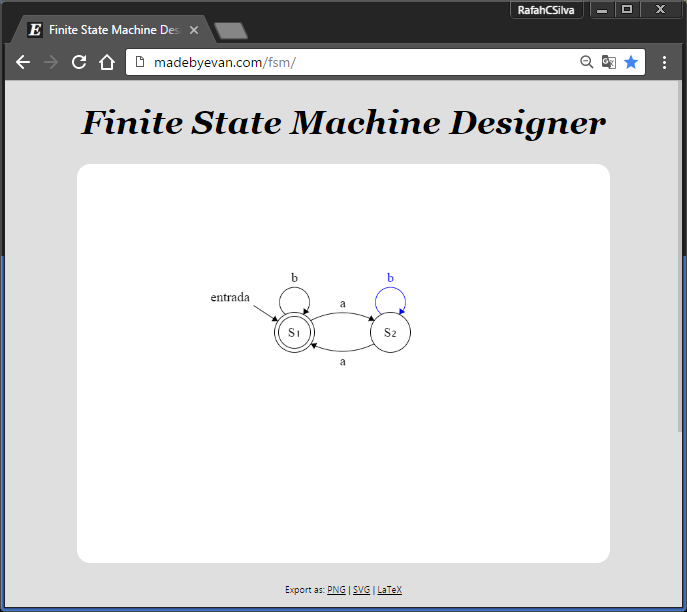
\includegraphics[scale=0.8]{fsm_page.png}  %0.7
    \caption{Construtor de máquinas de estados.}
    \label{fig:evan01}
  \end{figure}

  Esta ferramenta utiliza o elemento \textit{CANVAS}\footnote{Um elemento do HTML para exibir gráficos em uma página web.} do \textit{HTML5}\footnote{HTML5 (\textit{Hypertext Markup Language}, versão 5) é uma linguagem para estruturação e apresentação de conteúdo para a web.}, onde objetos são desenhados por meio de um \textit{JavaScript}\footnote{Linguagem de programação para páginas HTML e web, executada pelo navegador do cliente.}. Então, como esta ferramenta requer somente um navegador que suporte o elemento \textit{CANVAS}, ela é a ferramenta perfeita para ser utilizada na hora que os usuários do sistema (principalmente os alunos) precisarem fornecer o diagrama de um autômato. Como esta ferramenta tem licença MIT~\cite{mit}, qualquer pessoa pode usar, copiar, modificar, mesclar, publicar, distribuir, sublicenciar e vender como bem entender.

  Esta ferramenta tem estas características e pode ser usada para:

\begin{alineas}
  \item[$\bullet$] Criar estados com duplo clique em uma área em branco;
  \item[$\bullet$] Criar transições com a tecla \textit{shift} e o clicar e arrastar do \textit{mouse};
  \item[$\bullet$] Arrastar um objeto com o clicar e arrastar do \textit{mouse};
  \item[$\bullet$] Deletar um objeto selecionado clicando a tecla \textit{delete};
  \item[$\bullet$] Tornar um estado em aceitação, ou não, com um duplo clique sobre ele;
  \item[$\bullet$] Subscrever números com “$\_$”, do seguinte modo “$S\_0$” para obter “$S_0$”;
  \item[$\bullet$] Escrever letras gregas do seguinte modo “$\backslash$beta” para obter “$\beta$”;
  \item[$\bullet$] Exportar para PNG, SVG e \LaTeX\xspace a máquina de estados;
  \item[$\bullet$] Manipular os objetos desta máquina de estados em memória;
  \item[$\bullet$] Desenhar os objetos no elemento \textit{CANVAS} do \textit{HTML5};
  \item[$\bullet$] Salvar e recuperar automaticamente o diagrama no armazenamento local do navegador;
\end{alineas}

  O código fonte está disponível no repositório pessoal do Evan Wallace\footnote{Disponível em: \url{https://github.com/evanw/fsm}.}. Para este projeto precisaremos modificar o código para atender alguns requisitos do sistema. Dentre as funções destacadas acima, somente as funções de exportar, de salvamento e recuperação automática, de inserção de letras gregas e subscrito não nos interessa inicialmente. E, para este sistema, foi necessário a adição de funções extras, tais como: a verificação da correta confecção de um autômato finito determinístico e a extração de sua descrição matemática que para ser enviada ao juiz.

  Desenvolvemos assim uma especialização da ferramenta \textit{Finite State Machine Designer}, que possibilita a construção e verificação de autômatos finitos determinísticos, a qual demos o nome de \textbf{DFAdesigner}. Abreviação de \textit{Deterministic Finite Automaton Designer}, ou em português, Construtor de Autômato Finito Determinístico.


\chapter[Desenvolvendo o sistema] {Desenvolvendo o sistema}
  Neste capítulo são documentados as etapas do desenvolvimento do sistema web. Definimos os objetivos e requisitos a partir do contexto, para assim analisar e projetar este sistema, para assim, finalmente, implementa-lo e testa-lo. 

  O sistema pode ser acessado por dois tipos de usuários: Aluno e Professor, que desempenham papeis diferentes no sistema. O aluno é o discente matriculado na disciplina e o professor é o docente que ministra aquela turma.

  O objetivo principal deste sistema é a aplicação de listas de exercícios aos alunos de uma turma. E desta maneira, o sistema deve possibilitar também todo o gerenciamento destas aplicações.

  Um exercício nada mais é do que uma questão, constituída de um título, um enunciado e um autômato-gabarito que apresenta uma resposta correta. Questões ordenadas compõem uma lista, cada questão pode estar presente em diversas listas.

  Uma turma é formada por alunos e está subordinada a um professor, e nela são aplicadas listas de questões. Na aplicação de uma lista, é definida uma data e hora limite para o envio da solução do aluno. Um aluno pode fazer parte de mais de uma turma (por exemplo, no caso dele vir a refazer a disciplina).

  Então o professor deve gerenciar todas as turmas, listas e questões criadas por ele. E também o sistema pode suportar mais de um professor, no caso da disciplina ser ofertada por professores diferentes no mesmo período ou em períodos distintos.

  Já a administração de todos os usuários, como alunos ou outros professores, fica ao encargo de todos os professores. %Visto a possibilidade de um aluno fazer parte de diferentes turmas, criados por diferentes professores.


  Além de alunos e professores, há também um terceiro componente deste sistema, que denominaremos de Juiz, que tem a função de corrigir instantaneamente uma submissão. Ao longo deste capítulo, será melhor detalhado cada componente e seus relacionamentos.


\section{Modelo de Processo}
  Para o desenvolvimento deste projeto, foi utilizado o processo de desenvolvimento RAD\footnote{Abreviação de \textit{Rapid Application Development}, em português, Desenvolvimento de Aplicação Rápida.}, que é um modelo de processo de software incremental, que enfatiza um ciclo de desenvolvimento curto. Esse modelo permitiu o desenvolvimento rápido do projeto, que demorou 90 dias. Isso só foi possível porque houve muita reutilização de componentes no projeto, o que garantiu uma padronização tanto na aparência final do sistema, quanto da implementação de seus módulos, visto que o gerenciamento das Questões, Listas, Turmas e Usuários é praticamente igual.

  RAD também possibilita uma rápida prototipagem do sistema, proporcionando uma maior flexibilidade para projetar e um envolvimento maior do usuário. Assim, após definir os requisitos e restringir o escopro do sistema, pudemos fracionar o projeto em subprojetos. E, para a confecção de cada subprojeto, foram reutilizados componentes e padrões predefinidos foram seguidos, e  cada etapa só foi considerada encerrada após as validações do usuário.

  Esse modelo de processo possibilita que a construção e implementação do projeto ocorra paralelamente entre diversas equipes, proporcionando uma rápida conclusão, que é uma das grandes vantagens deste modelo. Porem este sistema tem seus principais módulos (Questão, Lista, Turmas e Usuários) dependentes entre si, dificultando este paralelismo. Mas mesmo contando somente com um desenvolvedor, este projeto se beneficiou de todas as outras vantagens que o RAD proporciona.


\section{Requisitos e Modelagem do Sistema}
  Nesta seção, listaremos os requisitos do sistema e sua modelagem.

\subsection{Requisitos Funcionais}
    Os Requisitos Funcionais são os itens que o sistema deverá oferecer ou restringir:

\begin{alineas}%[{RF}1]
  \item[\texttt{RF01.}] Acessar o sistema via web e funcionar em navegadores modernos;
  \item[\texttt{RF02.}] Garantir acesso somente a usuários previamente cadastrados pelo professor;
  \item[\texttt{RF03.}] Ser acessado utilizando um e-mail único e uma senha pessoal;
  \item[\texttt{RF04.}] Poder redefinir a senha, caso esquecida, e enviar no e-mail do usuário as informações de como ele deve proceder;
  \item[\texttt{RF05.}] Ter dois tipos de usuários: Professor e Aluno;
  \item[\texttt{RF06.}] Cadastrar um usuário com RA, nome completo e um e-mail;
  \item[\texttt{RF07.}] Enviar e-mail ao usuário explicando como ter acesso ao sistema e definir sua senha pessoal;
  \item[\texttt{RF08.}] Uma questão deve ter título e enunciado, que suportem comando \LaTeX, e um autômato-gabarito;
  \item[\texttt{RF09.}] Uma lista deve ter título e conter questões em uma ordem definida;
  \item[\texttt{RF10.}] Uma turma deve ser formada por alunos e nela deve ser aplicado listas com datas limites de submissão de respostas;
  \item[\texttt{RF11.}] Adicionar Alunos em lote em uma turma;
  \item[\texttt{RF12.}] O professor será o administrador, possibilitando:
  %\pointedenum
  \begin{alineas}
    \item[\texttt{RF12.1.}] Cadastrar, editar e remover usuários;
    \item[\texttt{RF12.2.}] Cadastrar, editar e remover questões;
    \item[\texttt{RF12.3.}] Cadastrar, editar e remover listas;
    \item[\texttt{RF12.4.}] Cadastrar, editar e remover turmas;
    \item[\texttt{RF12.5.}] Gerar relatório de desempenho de uma turma, e exportar em compatibilidade com editores de planilhas eletrônicas;
  \end{alineas}
  \item[\texttt{RF13.}] O aluno somente deve poder:
  %\pointedenum
  \begin{alineas}
    \item[\texttt{RF13.1.}] Visualizar as turmas em que ele está incluso;
    \item[\texttt{RF13.2.}] Visualizar as listas aplicadas à sua turma;
    \item[\texttt{RF13.3.}] Visualizar as questões contidas na lista;
    \item[\texttt{RF13.4.}] Submeter um autômato-resposta de uma questão;
    \item[\texttt{RF13.5.}] Salvar um autômato-resposta como rascunho;
    \item[\texttt{RF13.6.}] Visualizar os veredictos do juiz;
    \item[\texttt{RF13.7.}] Responder à lista de questões se esta não tiver o prazo de entrega expirado;
  \end{alineas}
\end{alineas}

\subsection{Requisitos Não-Funcionais}
  Os Requisitos Não-Funcionais são critérios que qualificam os Requisitos Funcionais:

  \begin{alineas}
    \item[\texttt{RNF01.}] Garantir a autenticação do usuário para todas suas ações;
    \item[\texttt{RNF02.}] Armazenar as senhas com criptografia;
    \item[\texttt{RNF03.}] Possibilitar a utilização do sistema com rápido tempo de treinamento;
    \item[\texttt{RNF04.}] Corrigir com rapidez e confiabilidade;
    \item[\texttt{RNF05.}] Garantir a integridade dos dados;
    \item[\texttt{RNF06.}] Garantir a disponibilidade;
    \item[\texttt{RNF07.}] Exigir o mínimo de recursos como espaço e CPU, a fim de baratear o custo do servidor;
    \item[\texttt{RNF08.}] Seguir um padrão estético em todas as interfaces;
    \item[\texttt{RNF09.}] Sanitizar todas as entradas de dados pelos usuários;
    \item[\texttt{RNF10.}] Usar um conexão segura com o banco de dados;
\end{alineas}




\subsection{Modelos Funcionais}

  Um modelo funcional serve para representar graficamente as funções relacionadas às regras de negócio, dentro de um contexto definido. Assim é possível modelar e descrever os processos realizados por cada componente.

  Para descrever as funções do sistema, foram utilizados os seguintes modelos funcionais: Diagrama de Caso de Uso e Diagrama de Fluxo de Dados.

  O diagrama de caso de uso abaixo mostra os atores do sistema e as funcionalidades associadas à eles.

\begin{figure}[H]
  \centering
  \includegraphics[width=0.95\textwidth]{diagCasoDeUso.png}%[scale=0.4]
  \caption{Diagrama de Caso de Uso.}
  \label{fig:DCU}
\end{figure}

  Para esclarecer como o sistema funciona e mostrar como as informações no sistema fluem, o Diagrama de Fluxo de Dados é apresentado a seguir.

\begin{figure}[H]
  \centering
  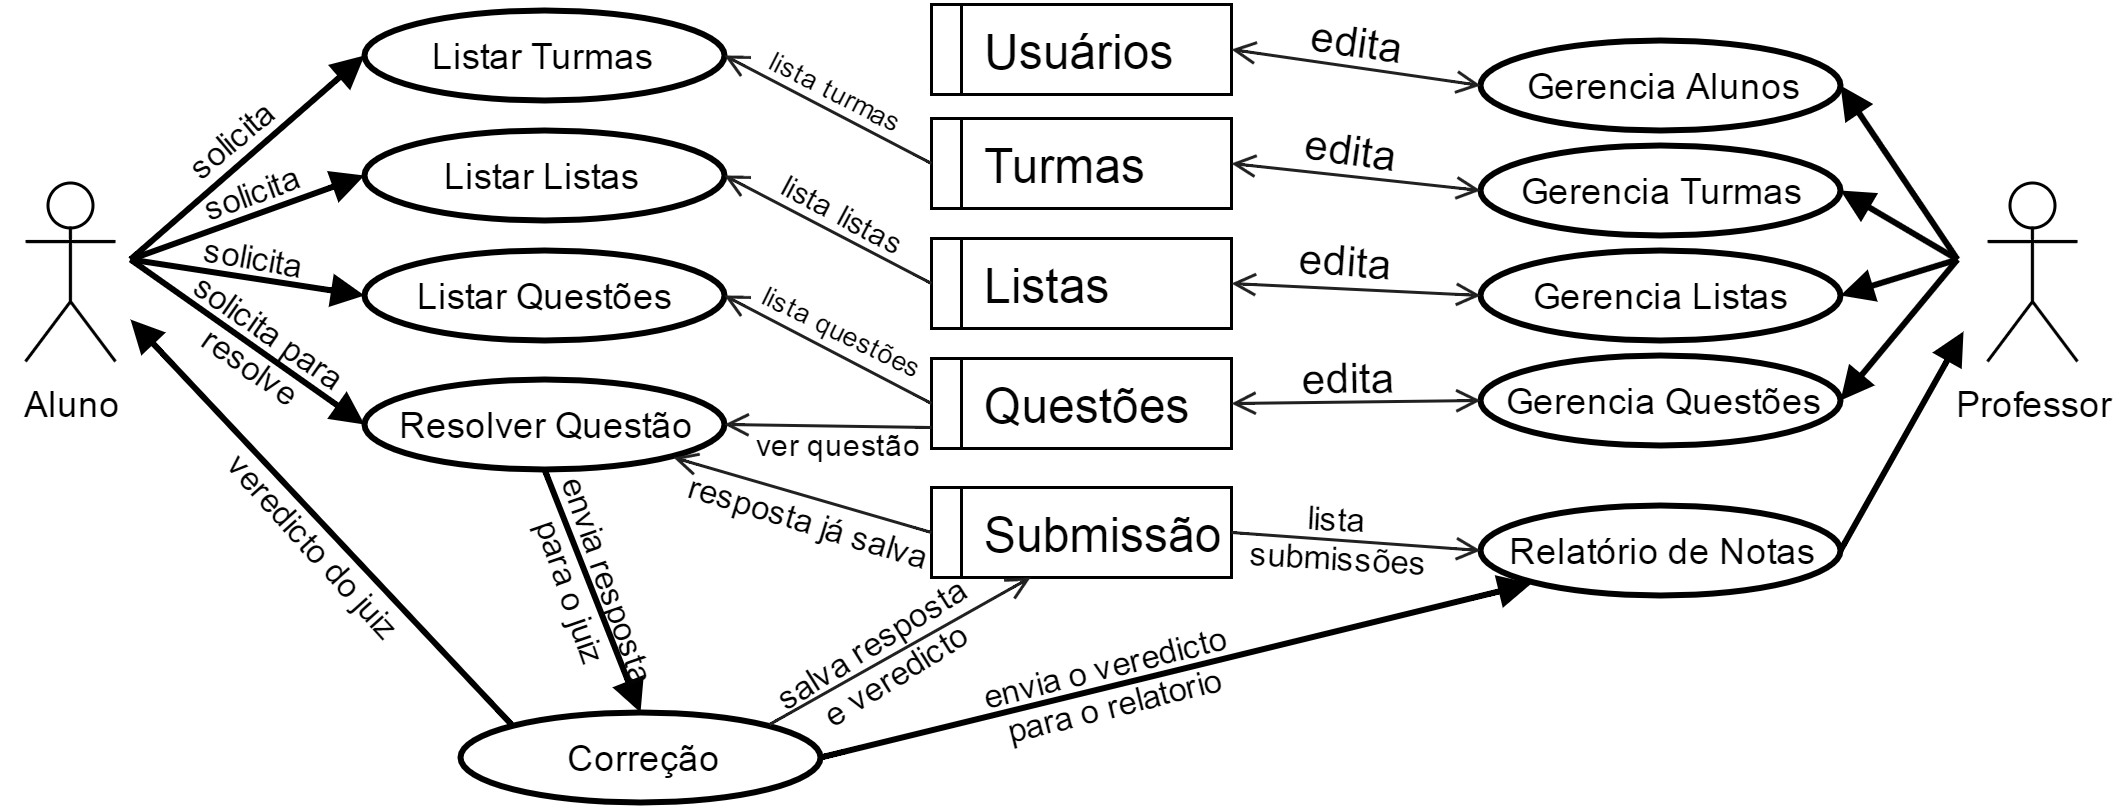
\includegraphics[width=\textwidth]{diagFluxoDeDados.png}%[scale=0.215]
  \caption{Diagrama de Fluxo de Dados.}
  \label{fig:DFD}
\end{figure}




\subsection{Modelos de Dados}
  Um modelo de dados permite apresentar como foram elaboradas as estruturas dos dados que dão suporte aos processos do sistema, mostrando como os dados são organizados e quais seus relacionamentos. Neste sistema podemos claramente observar que temos 4 entidades, e seus atributos e relacionamentos pode ser visto a seguir no Diagrama de Entidade Relacionamento.

\begin{figure}[H]
  \centering
  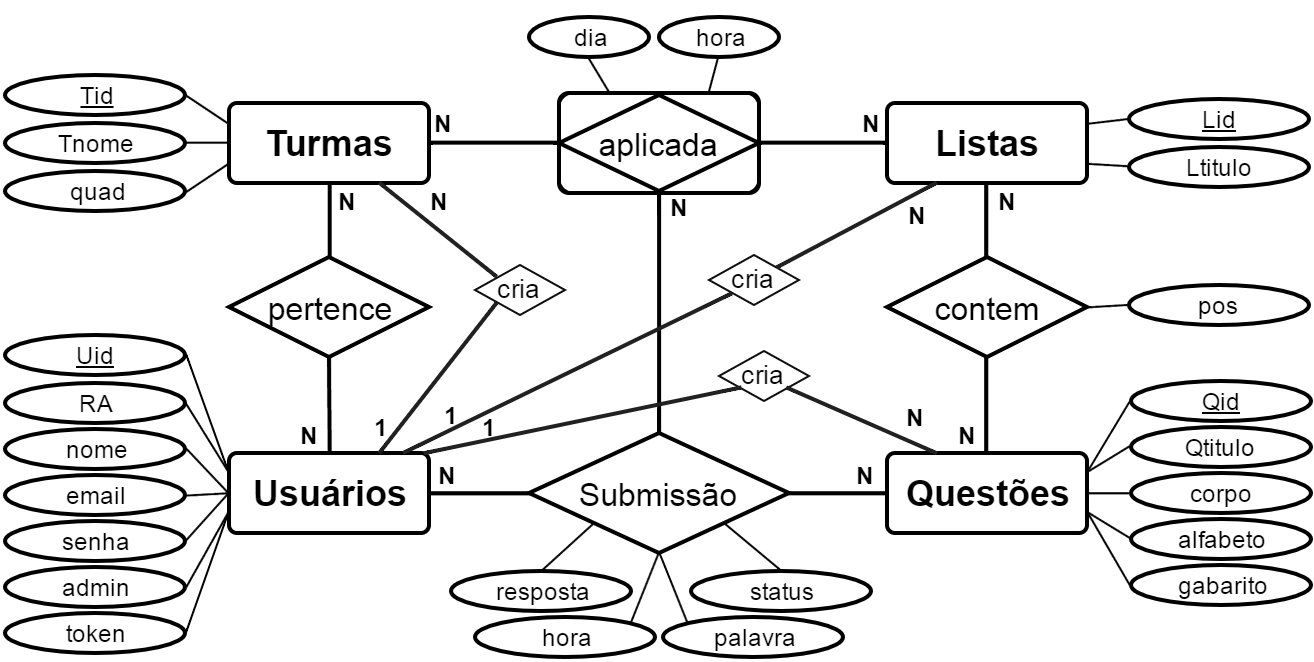
\includegraphics[width=\textwidth]{diagDER.png}%[scale=0.342]
  \caption{Diagrama de Entidade Relacionamento.}
  \label{fig:DER}
\end{figure}

  Este diagrama mostra as relações que determinam a dependência entre as entidades, e também possibilita que o professor gerencie as questões, as listas e as turmas por ele criadas, e também permite que os alunos visualizem os dados conforme as suas relações.

  E uma submissão do aluno é a relação entre uma questão de uma lista aplicada na sua turma, na qual armazena seu autômato-resposta e o veredicto do juiz, que é o status da submissão, juntamente com a palavra que o distinguiu, caso necessário.





\section{Análise}
  Nesta seção vamos analisar os requisitos, afim de tomar as decisões necessárias para seu desenvolvimento.

  Como o requisito primário deste sistema é ser um sistema web, então fundamentalmente o sistema foi projetado para esta plataforma. Assim tivemos de tomar algumas decisões, como em qual linguagem o sistema seria implementado e quais recursos estariam disponíveis para ele. E também necessitamos de um banco de dados para o armazenamento de todas as informações que o modelo prevê.

  Com o objetivo de baratear o custo para sua execução e garantir sua disponibilidade, o sistema não deve demandar de requisitos caros. Logo, foi escolhida a linguagem \textit{PHP}\footnote{PHP (\textit{PHP: Hypertext Preprocessor}) é uma linguagem de \textit{script open source}, muito utilizada e especialmente adequada para o desenvolvimento web.} para a implementação do sistema, pois esta linguagem oferece todas as condições necessárias para sua implementação, e os servidores comerciais oferecem planos mais acessível para suportar o PHP, e juntamente com ele o Sistema de Gerenciamento de Banco de Dados \textit{MySQL}\footnote{O MySQL é um sistema de gerenciamento de banco de dados.} para armazenamos os dados. E assim o sistema construirá páginas para responder às requisições do usuário.

  O uso de bibliotecas e \textit{frameworks} inicialmente não foram consideradas, ficando ao encargo do desenvolvedor toda sua codificação, por escolha própria dele, já que ele possui familiaridade com o desenvolvimento web com a linguagem \textit{PHP}, afim também de se aprimorar como um \textit{full stack web developer}\footnote{Perfil de desenvolvedor que lida com múltiplas camadas de desenvolvimento e tecnologias envolvidas, desde o \textit{back-end} até o \textit{front-end}, ou seja, do servidor ao cliente.}.

  Não foi possível obter um servidor dedicado do CMCC\footnote{Centro de Matemática Computação e Cognição da UFABC.}, assim o professor orientador deste projeto se dispôs a oferecer seu servidor comercial e endereço por ele já contratado, para ser utilizado durante o desenvolvimento e testes deste sistema, na qual não foi possível utilizar o padrão HTTPS\footnote{Abreviação de \textit{Hyper Text Transfer Protocol Secure}, em português, Protocolo de Transferência de Hipertexto Seguro, é uma implementação do protocolo HTTP sobre uma camada adicional de segurança.}, mas isto irá prejudicar em nada o desempenho final do sistema.

  O passo seguinte é criar um Modelo Relacional, a partir dos diagramas e modelos de dados vistos anteriormente. O Modelo Relacional permite a criação de um modelo lógico consistente da informação a ser armazenada. Este também pode ser refinado ao passar por um processo de normalização.

  Um Objeto de Dados, ou como chamamos anteriormente de Entidade, é a representação de um componente que contém propriedades. Estas propriedades chamamos de Atributos, que qualificam uma entidade e a distingue das outras. E o valor do atributo está definido em um domínio, ou tipo de dado. O Relacionamento é uma ligação lógica entre Entidades, representando a regra de negócio.

  Assim, este modelo relacional representa todas as regras de negócio deste sistema, mas adequado a um sistema de gerenciamento de banco de dados. Em que cada tabela é uma entidade, que contem atributos. Cada atributo tem seu tipo de dado especificado. E a ligação de um atributos à outras tabelas, representa um relacionamento, e a cardinalidade indica a quantidade de ocorrências deste relacionamento.

\begin{figure}[H]
  \centering
  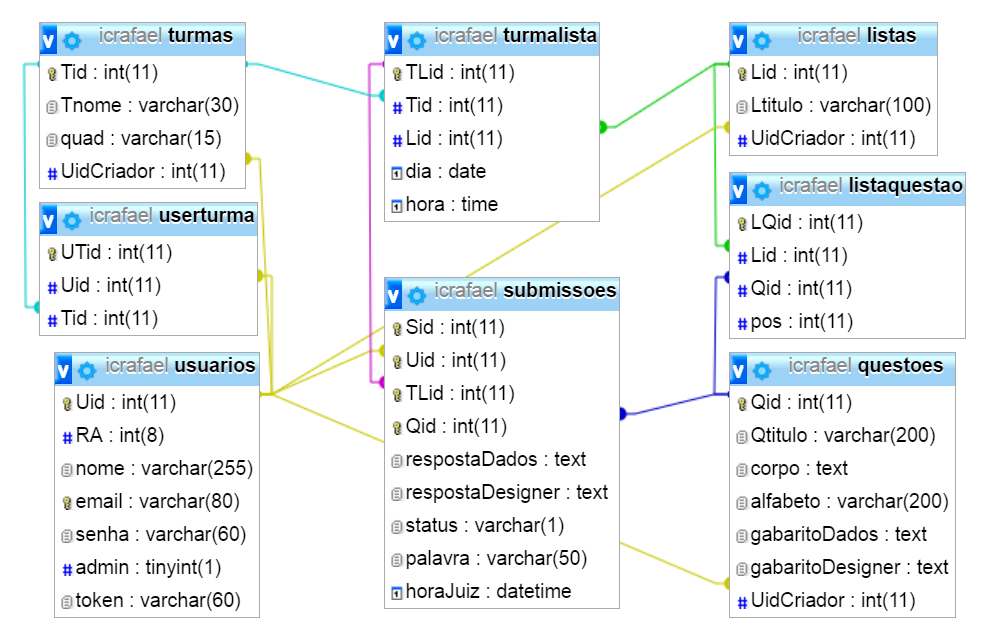
\includegraphics[width=\textwidth]{modRelacional.png}%[scale=0.62]
  \caption{Modelo Relacional.}
  \label{fig:MR}
\end{figure}

  O modelo Relacional deste sistema visto acima, na prática, gera as tabelas de um banco de dados relacional. As tabelas usuários, turmas, listas e questões representam as entidades vistas no diagrama da figura~\ref{fig:DER}. E as demais tabelas são utilizadas para apoiar os relacionamentos entre as entidades, geradas após a aplicação das devidas regras de normalização, garantindo assim a integridade dos dados a serem armazenados, o que possibilita a implementação do banco de dados, com todas as regras de negocio do sistema.



\section{Projeto}

  Nesta seção, tudo o que analisamos dos requisitos nas seções anteriores será detalhado. %, para ao fim implementar o sistema.

  Primeiro foi definido como seria a arquitetura do sistema. Em seguida, fizemos o detalhamento de todas as interfaces e suas interligações. E ao fim, elaboramos o Juiz e o DFAdesigner


  \subsection{Estilo Arquitetural}
  O estilo arquitetural em camadas separa o sistema em diferentes partes, que se integram afim de atender o que foi solicitado. Este estilo permite: uma maior independência funcional entre estas partes, facilita o desenvolvimento, particiona problemas complexos em sequencias de passos, facilita testes de integração e eventuais correções, e permite que um mesmo componente seja usado em diferentes propósitos.

  Neste padrão arquitetural de múltiplas camadas, cada camada tem responsabilidades especificas. O mais conhecido desde padrão é o MVC\footnote{Abreviação de \textit{Model-View-Control}, em português, Modelo-Visão-Controlador}, que separa a lógica do negócio, o modelo de dados e a interface gráfica.

  Assim a arquitetura deste sistema foi organizada em camadas, pois oferece maior flexibilidade, padronização e reuso de componentes. Podemos ver a baixo um esquema de como as camadas se integram.

\begin{figure}[H]
  \centering
  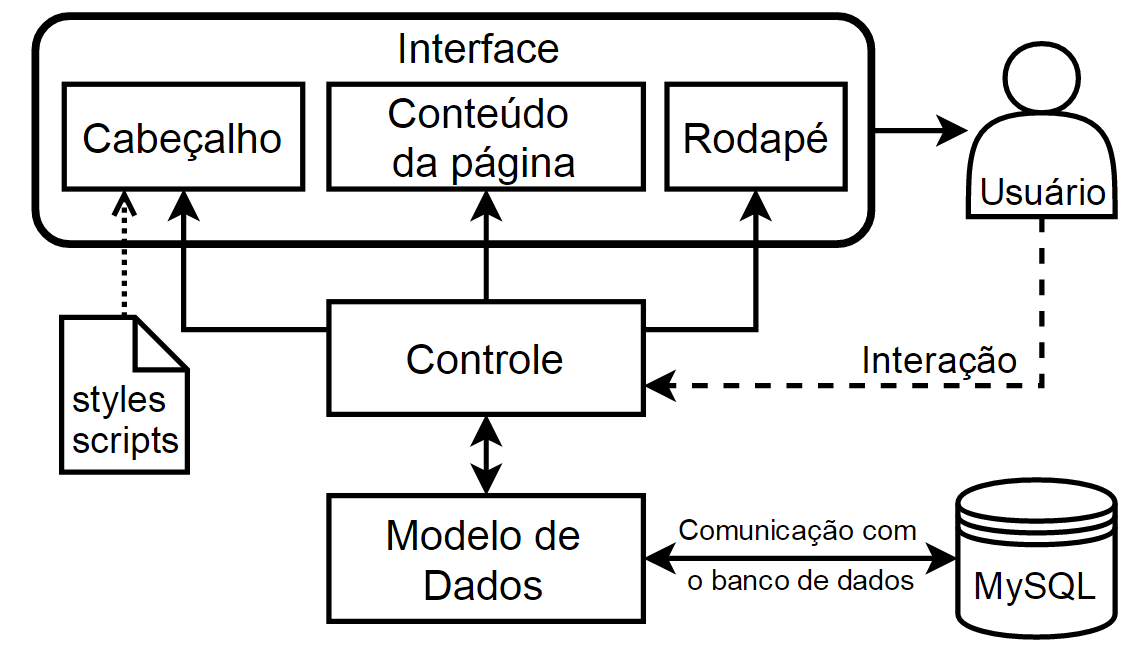
\includegraphics[scale=0.4]{camadas.png}
  \caption{Diagrama de Camadas.}
  \label{fig:dCamadas}
\end{figure}

  Quando usuário requisitar algo, o \textit{script} PHP receberá como parâmetro a ação e os dados necessários para poder atender o que foi solicitado. Tomamos como exemplo: o professor requisita a listagem de suas questões. Então a camada Controle recebe a ação de listagem de questões e deveria consultar o banco de dados para obter os dados solicitados, mas esta função é realizada pelo Modelo de Dados. Este se trata de um DAO\footnote{Abreviação de \textit{Data Access Object}, em português Objeto de Acesso a Dados.}, ou seja, um objeto que agrupa métodos relacionados ao acesso do banco de dados, como consultas e alterações de dados persistentes. Assim a comunicação direta com o banco de dados é tratada somente em um único lugar, possibilitando a reutilização de métodos em outros componentes. Um método do Modelo de Dados recebe os parâmetros necessários e retorna para o controle os dados ou conclui a ação requisitada. Continuando o exemplo, o Modelo de Dados retornaria a lista das questões daquele professor para o Controle, que agora deve gerar a Interface.

  Para formar a interface, o controle irá incluir 3 itens na saída: o cabeçalho, o conteúdo daquela página e o rodapé. O cabeçalho e o rodapé são os mesmos componentes que estarão presentes em todas interfaces. O cabeçalho contém os elementos pré textuais do HTML5, como os elementos: \textit{doctype}, \textit{html}, \textit{head}, \textit{title}, ícones, folhas de estilo e \textit{scripts}. Ele incluirá tudo que é necessário para o proposito daquela interface. Em seguida, ainda no cabeçalho, é iniciada a confecção do corpo da página, incluindo no caso deste sistema, um banner, o menu e uma barra de título com ações que serão apresentados mais a frente.

  Já o conteúdo da página é dinâmico em relação aos demais componentes, pois é definido no Controle a partir da ação requisitada, podendo conter formulários ou apresentando dados. No mesmo exemplo, será exibido uma tabela em que cada linha contém informações sobre cada questão e ações referentes a este item. E ao final, o rodapé é incluso, contendo os créditos do desenvolvimento. Um detalhe sobre interface é que o sistema foi projetado para ser acessado somente pelo computador, logo não há a grande necessidade da interface ser responsiva.

  Desta forma, o servidor PHP entrega esta interface ao usuário, para que ele interaja e requisite novas ações para o Controle.



  \subsection{Interface do Sistema}

  Garantir uma boa usabilidade e funcionalidade da interface de um sistema pode ser uma tarefa complexa. Uma boa interface deve garantir o rápido acesso a informação ou ação desejada. Deve haver consistência nos elementos da interface, ou seja, um objeto deve esta sempre no mesmo lugar. A interface por si só deve ser autoexplicativa, ou seja, facilmente deve-se entender o objetivo de cada um de seus componentes.

  Na Figura~\ref{fig:fluxoTelas} da página seguinte, vemos todo o fluxo de acesso aos componentes deste sistema por meio do diagrama ``Fluxo de Telas''.

\begin{sidewaysfigure} %[counterclockwise]
  \centering
  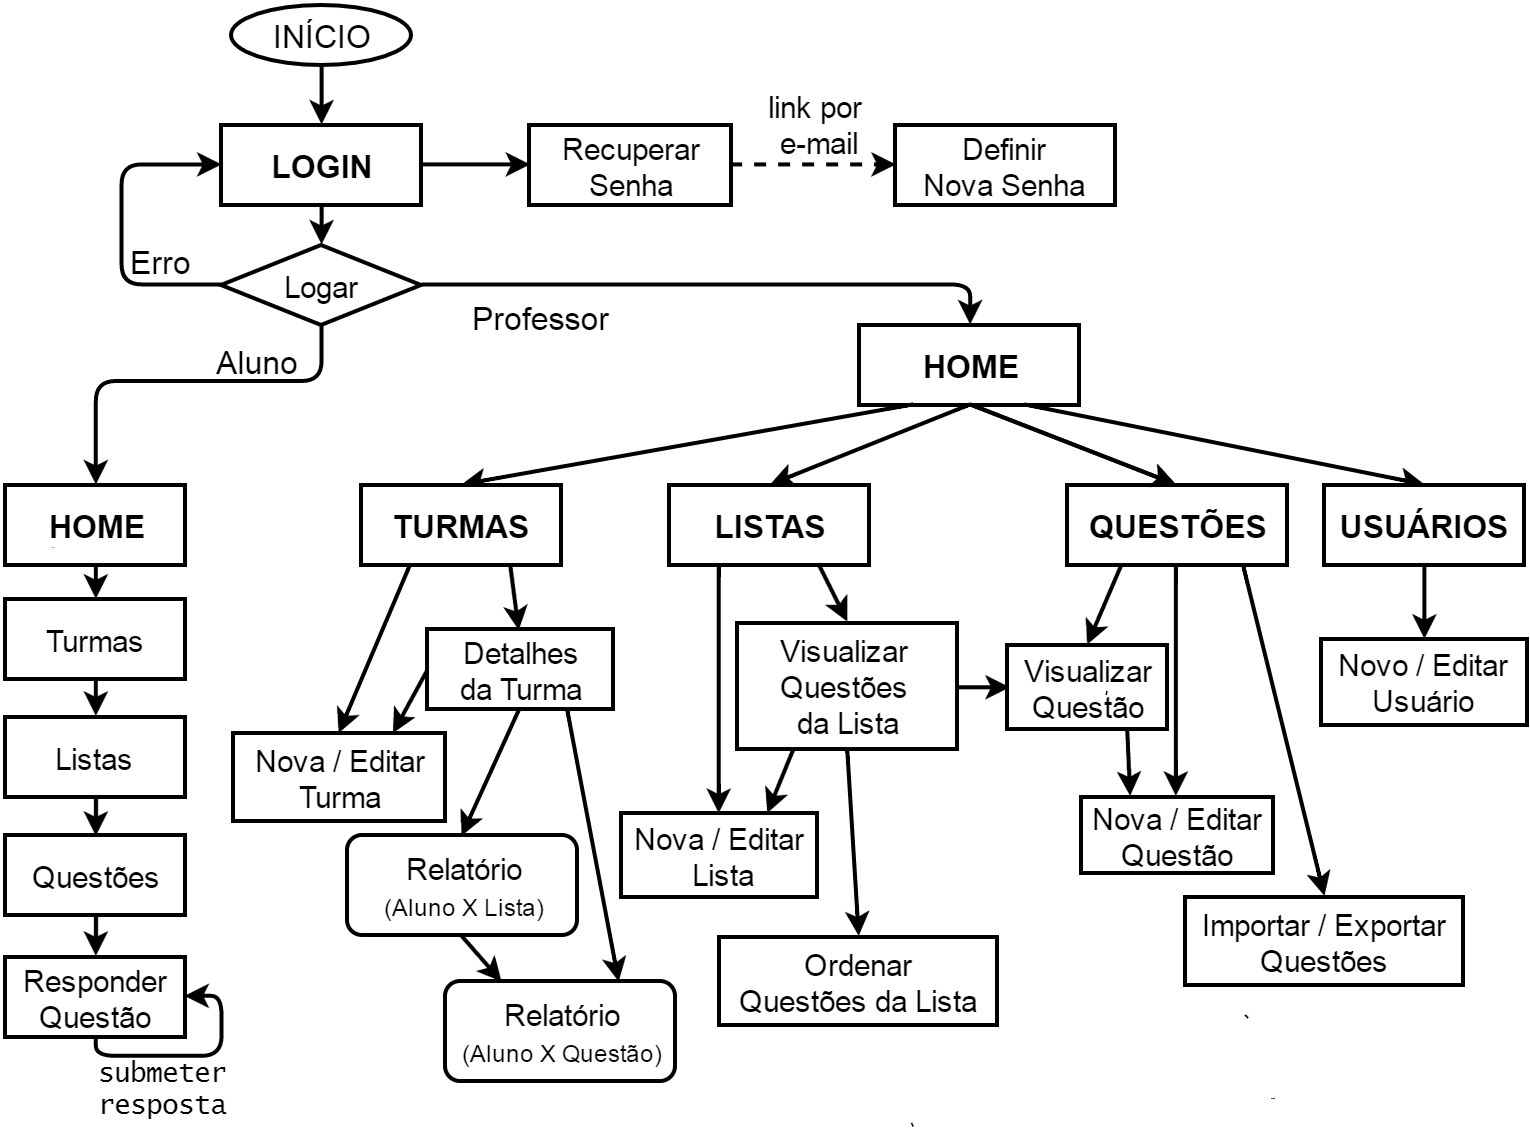
\includegraphics[scale=0.35]{fluxoTelas.png}
  \caption{Diagrama ``Fluxo de Telas''.}
  \label{fig:fluxoTelas}
\end{sidewaysfigure}

  Para entrar no sistema, o usuário deve inserir seu e-mail e uma senha por ele definida, em um pequeno formulário e clicar em logar na página de login. Uma vez dentro do sistema, é possível realizar as ações a ele atribuída, como veremos a diante.

  Também nesta tela de login, o usuário tem a possibilidade de redefinir a sua senha, caso ele a tenha esquecido. Para requisitar uma nova senha, basta inserir seu e-mail e clicar em enviar. Isto faz com que uma mensagem seja enviada ao e-mail, caso este esteja realmente no sistema, contendo os procedimentos para a definição de uma nova senha. O link enviado por e-mail, direciona o usuário para a tela de Definição de Nova Senha, onde ele pode definir uma nova senha. Este link contém um parâmetro (\textit{token}) criado para aquela requisição específica e é único.

  Cada usuário do tipo aluno pode visualizar as turmas em que ele está inscrito. Selecionando uma turma, ele pode visualizar as listas aplicadas a ela, e consultar as respectivas datas limites. Ao adentrar em uma lista, as questões que a compõem serão listadas, e cada uma é acompanhada de uma sinalização que representa o status da quela questão (possivelmente com o veredicto do juiz). Ao clicar em uma questão, o aluno deverá responder à questão em um formulário.

  Neste formulário estão inclusos o título e o enunciado da questão, e em seguida o DFAdesigner vazio, preparado para que o aluno desenhe a seu autômato-resposta. E na parte inferior há dois botões de ação: o Salvar e o Submeter. Ao clicar em Salvar, o desenho do aluno é salvo como rascunho, possibilitando a ele retomar a confecção de sua resposta posteriormente. Ao clicar em Submeter, o DFAdesigner analisa o desenho confeccionado, validando se está apto a ser um autômato finito determinístico e o envia ao Juiz. Caso o diagrama tenha problemas, a ação de submeter é abortada e uma mensagem alerta o aluno dos erros cometidos em relação ao desenho.

  Com o autômato-resposta corretamente validado, o juiz testa a sua equivalência com o autômato-gabarito daquela questão, e retorna ao aluno, no mesmo formulário de resposta, o seu veredicto: Correto ou Incorreto. Caso o veredicto seja Incorreto, o juiz também retorna a palavra que distinguiu o autômato-resposta do autômato-gabarito.

  Já o usuário do tipo professor, ele tem a responsabilidade de gerir todos os objetos envolvidos: usuário, questões, listas e turmas.

  Na página de Usuários é possível adicionar novos usuários, editar um usuário já existente e também excluir usuários. Para editar ou adicionar um usuário, basta preencher um formulário com seu RA (no caso do aluno), o nome completo, um e-mail e qual o privilegio daquele usuário (se é administrador ou aluno). Ao adicionar um novo usuário, é enviado a ele um e-mail de boas-vindas, o informando de que foi adicionado ao sistema e contendo instruções para definir uma senha pessoal de acesso.

  Na página de Questões, são listadas todas as questões criadas por este professor. Assim, é possível adicionar, editar, remover e visualizar uma questão, e também existe a possibilidade de duplicar uma questão já existente. Esta página também exibe quantas vezes cada questão foi utilizada nas listas do professor. Ao visualizar uma questão, ela é impressa na tela como será visualizada pelo aluno ao responde-la e abaixo o DFAdesigner com desenho do autômato-gabarito, porém bloqueado para edições. Ao adicionar ou editar uma questão, o professor deve preencher um formulário com o título e enunciado da questão, e listar os símbolos do conjunto $\Sigma$ que compõe a resposta. Logo abaixo, está disponível o DFAdesigner para a confecção ou edição do autômato que representa uma possível resposta correta, ou seja, o autômato-gabarito. Nesse formulário, nos campos de título e enunciado, é possível a utilização de comandos \LaTeX\xspace e elementos HTML, para uma melhor formatação destes.

  Na página de Listas são enumeradas todas as listas criadas por aquele professor, onde é possível visualizar, adicionar, editar ou remover uma lista. Ao visualizar uma lista, são relacionadas todas as questões contidas naquela lista e também existe a possibilidade de reordena-las. No formulário de edição ou criação de uma nova lista, o professor deve definir um nome para esta lista e, abaixo, são listadas todas as suas questões para que ele possa selecionar quais deverão compor esta lista.

  A página de Turmas é mais complexa comparada às anteriores: o professor vai gerenciar as turmas que ele ministra. Então são listadas as suas turmas, e em cada uma delas a que quadrimestre ela está associada, o número de alunos e o número de listas aplicadas. E há possibilidade de visualizar, adicionar, editar e remover uma turma. Ao adicionar ou editar uma turma, o professor deve preencher um formulário com o nome da turma, o quadrimestre, e selecionar os alunos previamente cadastrados. os alunos também podem ser selecionados em lote por meio de um arquivo CSV\footnote{Abreviação de \textit{Comma-Separated Values}, ou em português, valores separados por virgula, é um formato de arquivo comumente usados por editores de planilhas eletrônicas.}, e assim automaticamente adicionando ao sistema alunos que não estão previamente cadastrados. E ao fim escolher dentre suas listas, quais vão ser aplicadas naquela turma, juntamente com a data e hora limite para realizar submissões. Ao visualizar uma turma são listados os alunos nela contidos e as listas aplicadas nela. E nesta mesma página há um redirecionamento para uma outra página em que será gerado e apresentado o relatório daquela turma. O relatório é a listagem de todos os alunos e o número de acertos em cada lista. E há possibilidade também de visualizar para cada lista, qual foi o veredicto do juiz para aquela resposta do aluno. E ao final existe a possibilidade de exportar este relatório como uma planilha no formato CSV, que vai auxiliar este professor a compor a nota final de cada aluno.

  Outra página que o sistema disponibiliza é uma seção de ajuda, que contém um tutorial utilizando animações para ensinar o usuário a utilizar o DFAdesigner e contém explicações de outras interações que o aluno pode realizar no sistema. Finalmente há uma página para que o usuário possa visualizar suas próprias informações, possibilitando também a redefinição de sua senha pessoal. %E por fim uma página sobre o sistema.





  \subsection{O DFAdesigner e o Juiz}

  Nesta seção, trataremos dos componentes mais importantes deste projeto, que é o método para construir e avaliar uma resposta-autômato. O DFAdesigner e o Juiz estão intimamente ligados, pois o DFAdesiger, além de possibilitar o usuário confeccionar um AFD, ele deve coletar do diagrama os dados necessários para que o Juiz possa avaliar esta resposta com base no gabarito.

  Então devemos projetar as modificações necessárias do FSM para utiliza-lo de modo eficiente, pois além de coletar os dados do AFD desenhado pelo usuário, o DFAdesigner deve verificar se o diagrama desenhado condiz de fato com um AFD, para assim envia-lo para o Juiz. Senão deve retornar mensagens sobre os erros cometidos, que são as seguintes condições em relação a construção deste autômato-resposta:
  
  %\clearpage

\begin{alineas}
  \item[$\bullet$] Se há estados desenhados;
  \item[$\bullet$] Se cada estado está nomeado, senão nomea-los;
  \item[$\bullet$] Se há transições com pelo menos um simbolo associado;
  \item[$\bullet$] Se há transições com um simbolo inválido;
  \item[$\bullet$] Se há transições com símbolos duplicados ou sobrescrevendo outra transição;
  \item[$\bullet$] Se há uma transição para cada simbolo a partir de um estado;
  \item[$\bullet$] Se há uma e somente uma transição inicial para indicar o estado inicial;
\end{alineas}

  E também adaptar os \textit{scripts} do Evan para que o DFAdesigner possa recuperar do banco de dados o autômato-resposta salvo ou submetido pelo aluno anteriormente.

  Após o autômato-resposta ser verificado, o Juiz obtém os dados coletado pelo DFAdesigner e o autômato-gabarito armazenado anteriormente, mas ambos em uma codificação mais concisa, para que, ao receber estes dados, possa converter novamente para uma estrutura que defina estes autômatos para serem utilizados. Estes dados codificados se tratam de uma sequência de número naturais que codifica o autômato da seguinte forma:
 %pois assim ao interpretar estes dados possibilita restruturar os dois autômatos para serem utilizados.
 
\begin{alineas}
  \item[$\bullet$] O primeiro número indica a quantidade de estados deste autômato, pois o nome dos estados não nos importa, somente uma enumeração implícita é necessário;
  \item[$\bullet$] Depois vem os valores da tabela de transições deste autômato, na qual as linhas estão ordenadas pelo índice dos estados e as colunas conforme os símbolos do conjunto $\Sigma$ daquela questão;
  \item[$\bullet$] Em seguida o índice do representante do estado inicial;
  \item[$\bullet$] E, por ultimo, o conjunto de estados que são de aceitação, iniciando pelo número $m$ de estados de aceitação e, em seguida, uma lista com $m$ números que correspondem aos índices dos estados de aceitação.
\end{alineas}

  Estes dados são transmitido em uma única linha de números separados por um espaço, pois deste modo facilita o armazenamento e o interpretação do autômato que é representado por esta cadeia de números de forma compacta.

  Vejamos um exemplo de como resultaria a codificação do autômato $M_1$  apresentado na Figura~\ref{fig:aut01} anteriormente:

\begin{figure}[H]
  \centering
  
\includegraphics[scale=0.3]{exemploCodificacao.png}
  \caption{Codificação do autômato $M_1$.}
  \label{fig:exemploCodificacao}
  \vspace{-0.5cm}
\end{figure}

  Podemos observar na Figura~\ref{fig:exemploCodificacao} a separação desta sequência de números nos exatos 4 blocos que definimos anteriormente. Como $M_1$ tem dois estados, então o primeiro número é 2. Os estados de $M_1$ são enumerados, assim o estado $S_1$ é o $0$ e o estado $S_2$ é o $1$. Depois vem a sua tabela de transições, que é representada pela Tabela~\ref{tab:tabTransicoesM1}. Na qual temos dois estados e dois símbolos no conjunto $\Sigma$, logo teremos o número de estado multiplicado pelo número de símbolos, que será a quantidade de números desta sequência dos índices dos estados que formam a tabela de transições deste autômato. %, que assim é formado pelos valores das colunas de cada linha. 
  Em seguida vem o índice do estado inicial, que é o $0$. E por fim os estados de aceitação, mas primeiro o número total de estados de aceitação e em seguida os índices destes estados, neste caso temos somente $1$ estado de aceitação, e este estado é o de índice $0$.

  O juiz recebe o autômato-resposta e o autômato-gabarito codificados deste modo, e também o conjunto de símbolos do alfabeto, e os interpretam afim de uni-los numa estrutura de dados em que ele possa finalmente aplicar o Algoritmo~\ref{alg03} e, em seguida, o Algoritmo~\ref{alg04} se necessário. Para ao final retornar seu veredicto.

  O veredicto do Juiz é identificado pelo \textit{status} da submissão do aluno, como podemos ver a seguir:

 \begin{alineas}
  \item[\textbf{\texttt{A  }}] Aguardando o processo de correção do Juiz;
  \item[\textbf{\texttt{S  }}] Salvo como rascunho;
  \item[\textbf{\texttt{C  }}] Resposta correta;
  \item[\textbf{\texttt{I  }}] Resposta incorreta, e acompanha a palavra que os distinguiram;
\end{alineas}

  Deste modo a interface do usuário no navegador, que é o DFAdesigner, se comunica com o Juiz, que está presente no servidor. Então os dados coletados pelo DFAdesigner é salvo no banco de dados na submissão do aluno. Nesta submissão contém esta codificação do autômato e um JSON\footnote{Abreviaçõa de \textit{JavaScript Object Notation}, ou em português, Notação de Objetos JavaScript, é um formato leve de troca de dados com fácil leitura e interpretação tanto de humanos, tanto do computadores.} que representa os objetos da estrutura do desenho do diagrama, que originalmente o Evan implementou para salvar no armazenamento local do navegador, e para obter uma rápida restauração do mesmo. E junto a estes dados da submissão também consta o \textit{status} do Juiz, e a palavra que distinguiu o autômato-resposta do aluno do autômato-gabarito da questão.
  
  Inicialmente, pensamos que arquitetar este Juiz de forma assíncrona às submissões, ou seja, as respostas submetidas pelos alunos aguardarão em uma fila para serem atendidas pelo Juiz posteriormente. Esta é uma estratégia utilizadas por outros sistemas que realizam algum tipo de julgamento, onde realizar esta tarefa necessita de um tempo superior a espera da resposta em um sistema cliente-servidor. Assim, arquitetar nosso sistema para lidar com as submissões de tal modo, ocasionaria o aumento da complexidade do sistema e principalmente de recursos do servidor. 
  
  Então durante o estudo e implementação do Algoritmo~\ref{alg03} e~\ref{alg04} em C++, notamos que a sua execução é de fato muito mais rápida, ao ponto de que em uma requisição, ele possa ser executado e retornar seu veredicto como resposta ao cliente. E oportunamente o algoritmo de Hopcroft e Karp pode ser portado para a linguagem PHP, afim de obter maior integração com o sistema e maior agilidade para responder a requisição.
  
  Assim este sistema deve receber a submissão do aluno e retornar seu veredicto. Mas para melhor explicar como se sucede esta sequencia de processos, veremos o Diagrama de Sequência da submissão a seguir.
  
\begin{figure}[H]
  \centering
  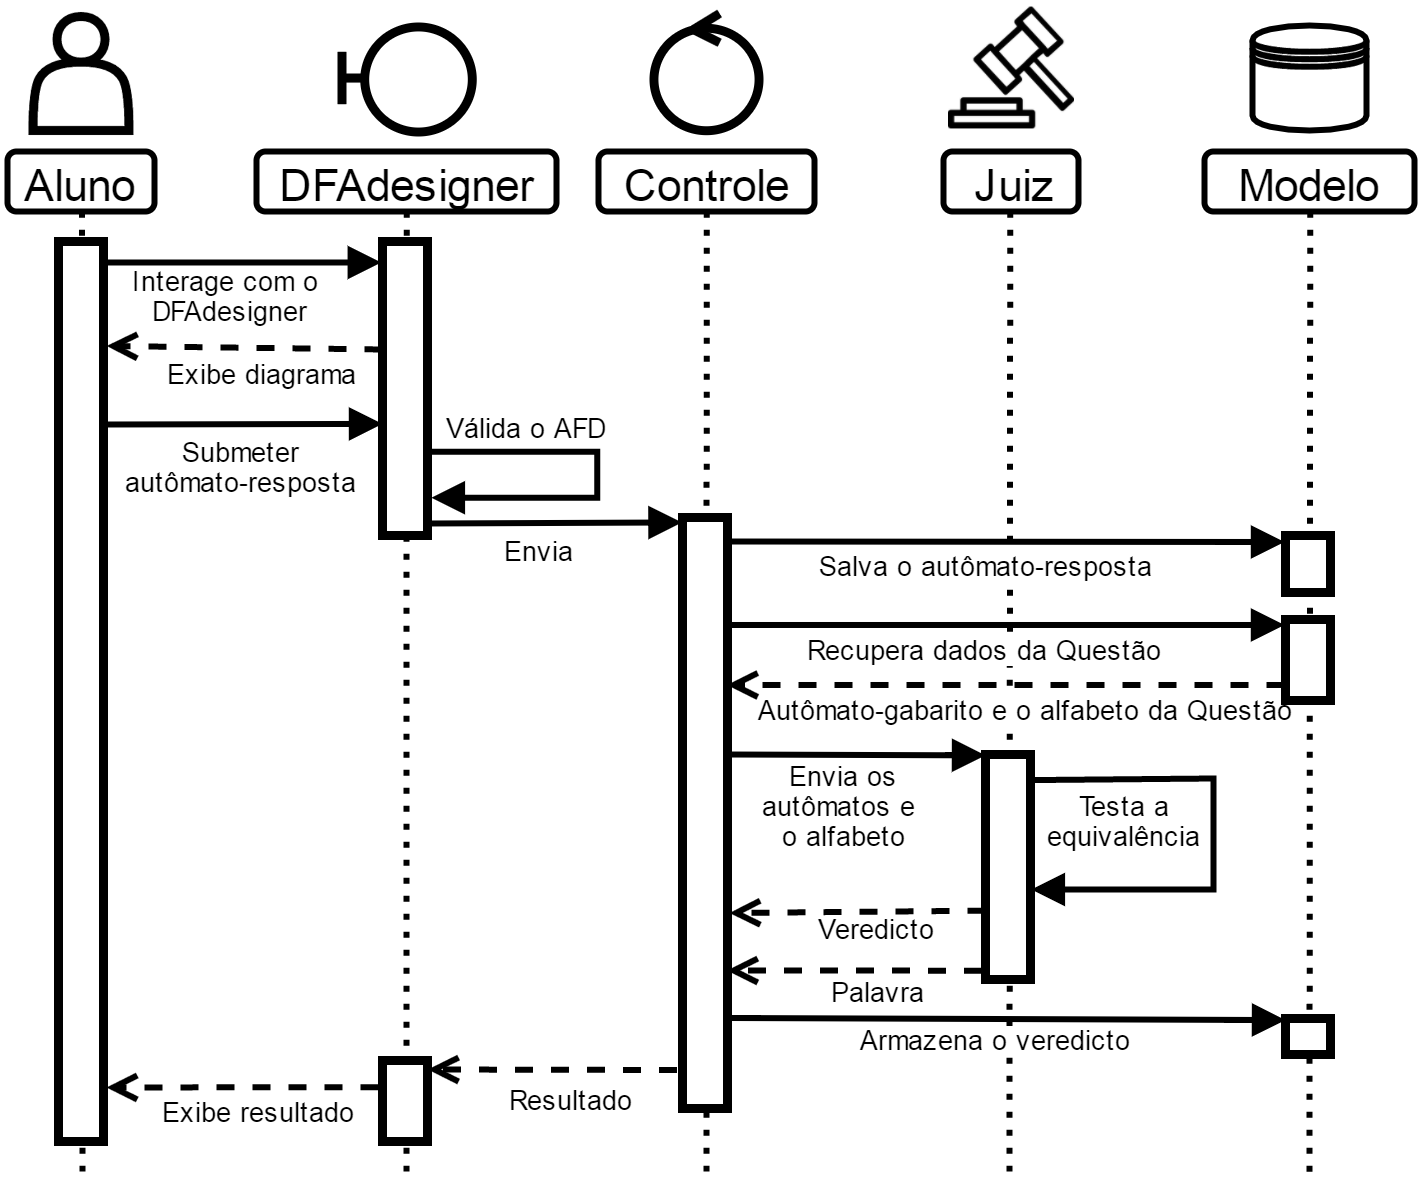
\includegraphics[scale=0.31]{diagSequencia.png}%[width=\textwidth]
  \caption{Diagrama de Sequência da submissão.}
  \label{fig:diagSequencia}
  \vspace{-0.5cm}
\end{figure}
  
  O diagrama nos ajuda a entender melhor como se sucede a comunicação do DFAdesigner com o Juiz sobre a arquitetura de camadas do sistema. Após o Aluno interagir com o DFAdesigner para confeccionar o seu autômato-resposta, ele pode submete-lo para a correção, mas primeiro seu diagrama será verificado, e se caso apontar algum erro, então a ação seria abortada e exibiria os erros cometidos. Senão os dados necessários são coletados, da forma codificada apresentada anteriormente, e também a estrutura do desenho do diagrama, para ser enviado ao Controle. 
  
  No Controle, ele utiliza o Modelo de Dados para salvar no banco de dados o autômato-resposta do aluno, que é constituído pelos dados e o desenho. Se caso fosse a ação de salvar como rascunho, este processo terminaria aqui, e retornaria uma mensagem ao usuário informando-o de que o rascunho foi salvo com sucesso. 
  
  Mas, no caso de uma submissão, o Controle recupera o autômato-gabarito e o alfabeto daquela questão, e entrega ao Juiz o conjunto de símbolos do alfabeto, o autômato-resposta e o autômato-gabarito, para ele realizar o teste de equivalência como descrevermos nos capítulos anteriores. 
   
  Ao final, o Juiz retorna seu veredicto, e também a palavra que os distinguiu (se necessária), para o controle que vai alterar o \textit{status} da submissão para o corresponder ao veredicto. E, por ultimo, o controle retorna para o aluno o resultado obtido. Todo esse processo ocorre em uma única requisição do cliente para o servidor.



\section{Implementação}

  Após feita a análise dos requisitos e o projeto deste sistema, vem a sua codificação. Nesta seção vamos tratar de alguns assuntos referentes ao \textit{design} das interfaces e das implementações realizadas para atender os requisitos deste projeto. %, bem com o a modificação do FSM do Evan proposta anteriormente para se adequar ao sistema.
  
  Após estudado o \textit{script} do FSM, algumas de suas funções foram alteradas para possibilitar que o JSON, que representa o diagrama, possa ser salvo em banco de dados e recuperado posteriormente para ser reexibido. Também as novas funções, que discutimos anteriormente, foram adicionadas. Para analisar e coletar os dados do diagrama, bastou varrer a estrutura de dados que o FSM implementa, obtendo então: o índice dos estados e quais são de aceitação, as transições entre os estado que é nomeada com um simbolo e o estado inicial demarcado.
  
  %Primeiramente, foi estudado o \textit{script} do FSM afim de interpretar seu funcionamento. Em seguida algumas de suas funções foram editadas para possibilitar que o JSON, que representa o diagrama, possa ser salvo em banco de dados e recuperado posteriormente para ser reexibido. Depois foram adicionado novas funções referentes a submissão, que deve além de salvar o JSON, analisar o diagrama afim de verificar todas aquelas condições anteriormente enumeradas, e se caso alguma violação ocorrer, então possibilitar que uma mensagem liste os erros cometidos e que a ação seja abortada. Para analisar e coletar os dados do diagrama, bastou varrer a estrutura de dados que o FSM implementa, obtendo então: o índice dos estados e quais são de aceitação, as transições entre os estado que é nomeada com um simbolo e o estado inicial demarcado.
  
  %Inicialmente, foi modificado funções do FSM para obter o JSON dos seus objetos, que forma a estrutura do diagrama, para ser armazenado no banco de dados quando houver a submissão ou salvar como rascunho. Bastou apenas redirecionar a saída das funções de carregar e armazenar já presentes no \textit{script} do Evan.

  %Porém quando houver a submissão, os dados codificados do autômato-resposta também é enviada. Para adquirir estes dados, foi realizada uma varredura na estrutura que abriga as propriedades dos objetos do desenho, assim recolhendo as informações pertinentes ao autômato desenhado, como: o índice dos estados, quais estados são de aceitação, as transições entre os estado com o simbolo utilizado para nomear esta ligação, a transição inicial para demarcar o estado inicial. E junto a este processo é realizado as verificações, enumeradas anteriormente, sobre a construção do diagrama, e em caso de alguma violação, a ação de submeter é abortada e as mensagens que descreve os erros cometidos são exibidos ao usuário.

\begin{wrapfigure}{l}{0.28\textwidth}
  \vspace{-0.5cm}
  \centering
  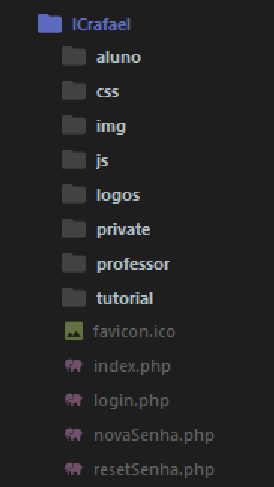
\includegraphics[scale=0.6]{filesSublime.png}
  \caption{Arquivos.}
  \label{fig:files}
  \vspace{-2cm}
\end{wrapfigure}
    
  A Figura~\ref{fig:files} mostra a estrutura do diretório, onde se encontram os \textit{scripts} do sistema. Na raiz está a página inicial com o login, a recuperação de senha e a definição de senha. Já nas subpastas contém os seguintes arquivos:
  
 \begin{alineas}
   \item[$\bullet$] \textbf{css} - Os arquivos \textit{Style Sheets};
   \item[$\bullet$] \textbf{js} - Os arquivos JavaScript, incluído o DFAdesigner;
   \item[$\bullet$] \textbf{img} - Ícones para a interface;
   \item[$\bullet$] \textbf{logo} - Logos do banner e de outras interfaces;
   \item[$\bullet$] \textbf{tutorial} - Imagens animadas utilizada no tutorial;
   \item[$\bullet$] \textbf{aluno} - Arquivos do Controle do aluno;
   \item[$\bullet$] \textbf{professor} - Arquivos do Controle do professor;
   \item[$\bullet$] \textbf{private} - Classes do DAO, do Juiz e bibliotecas;
 \end{alineas}

  O banco de dados foi implementado no SGBD MySQL, seguindo os modelos já apresentados. Assim o PHP se conecta a este banco de dados utilizando a biblioteca PDO, que fornece uma interface e os \textit{drivers} necessários para realizar esta conexão de forma segura e garante também a higienização dos valores a serem inseridos no banco de dados.
  
  O \textit{design} das interface se tornou algo importante durante a implementação. Com a rápida prototipagem que RAD proporciona, versões funcionais deste sistema eram demonstrados ao orientador deste projeto, afim dele avaliar e testar as funções implementadas. E suas opiniões ajudavam a melhorar as funcionalidades e também a usabilidade das interfaces do sistema, e até mesmo sugerindo novas funcionalidades.
  
  Então, afim de idealizar as interfaces deste sistema, foram confeccionados os \textit{mockups}, que é equivalente à uma ``maquete de uma interface'', não necessariamente de alta fidelidade, para simular o uso da interface.
  
\begin{figure}[H]
  \centering
  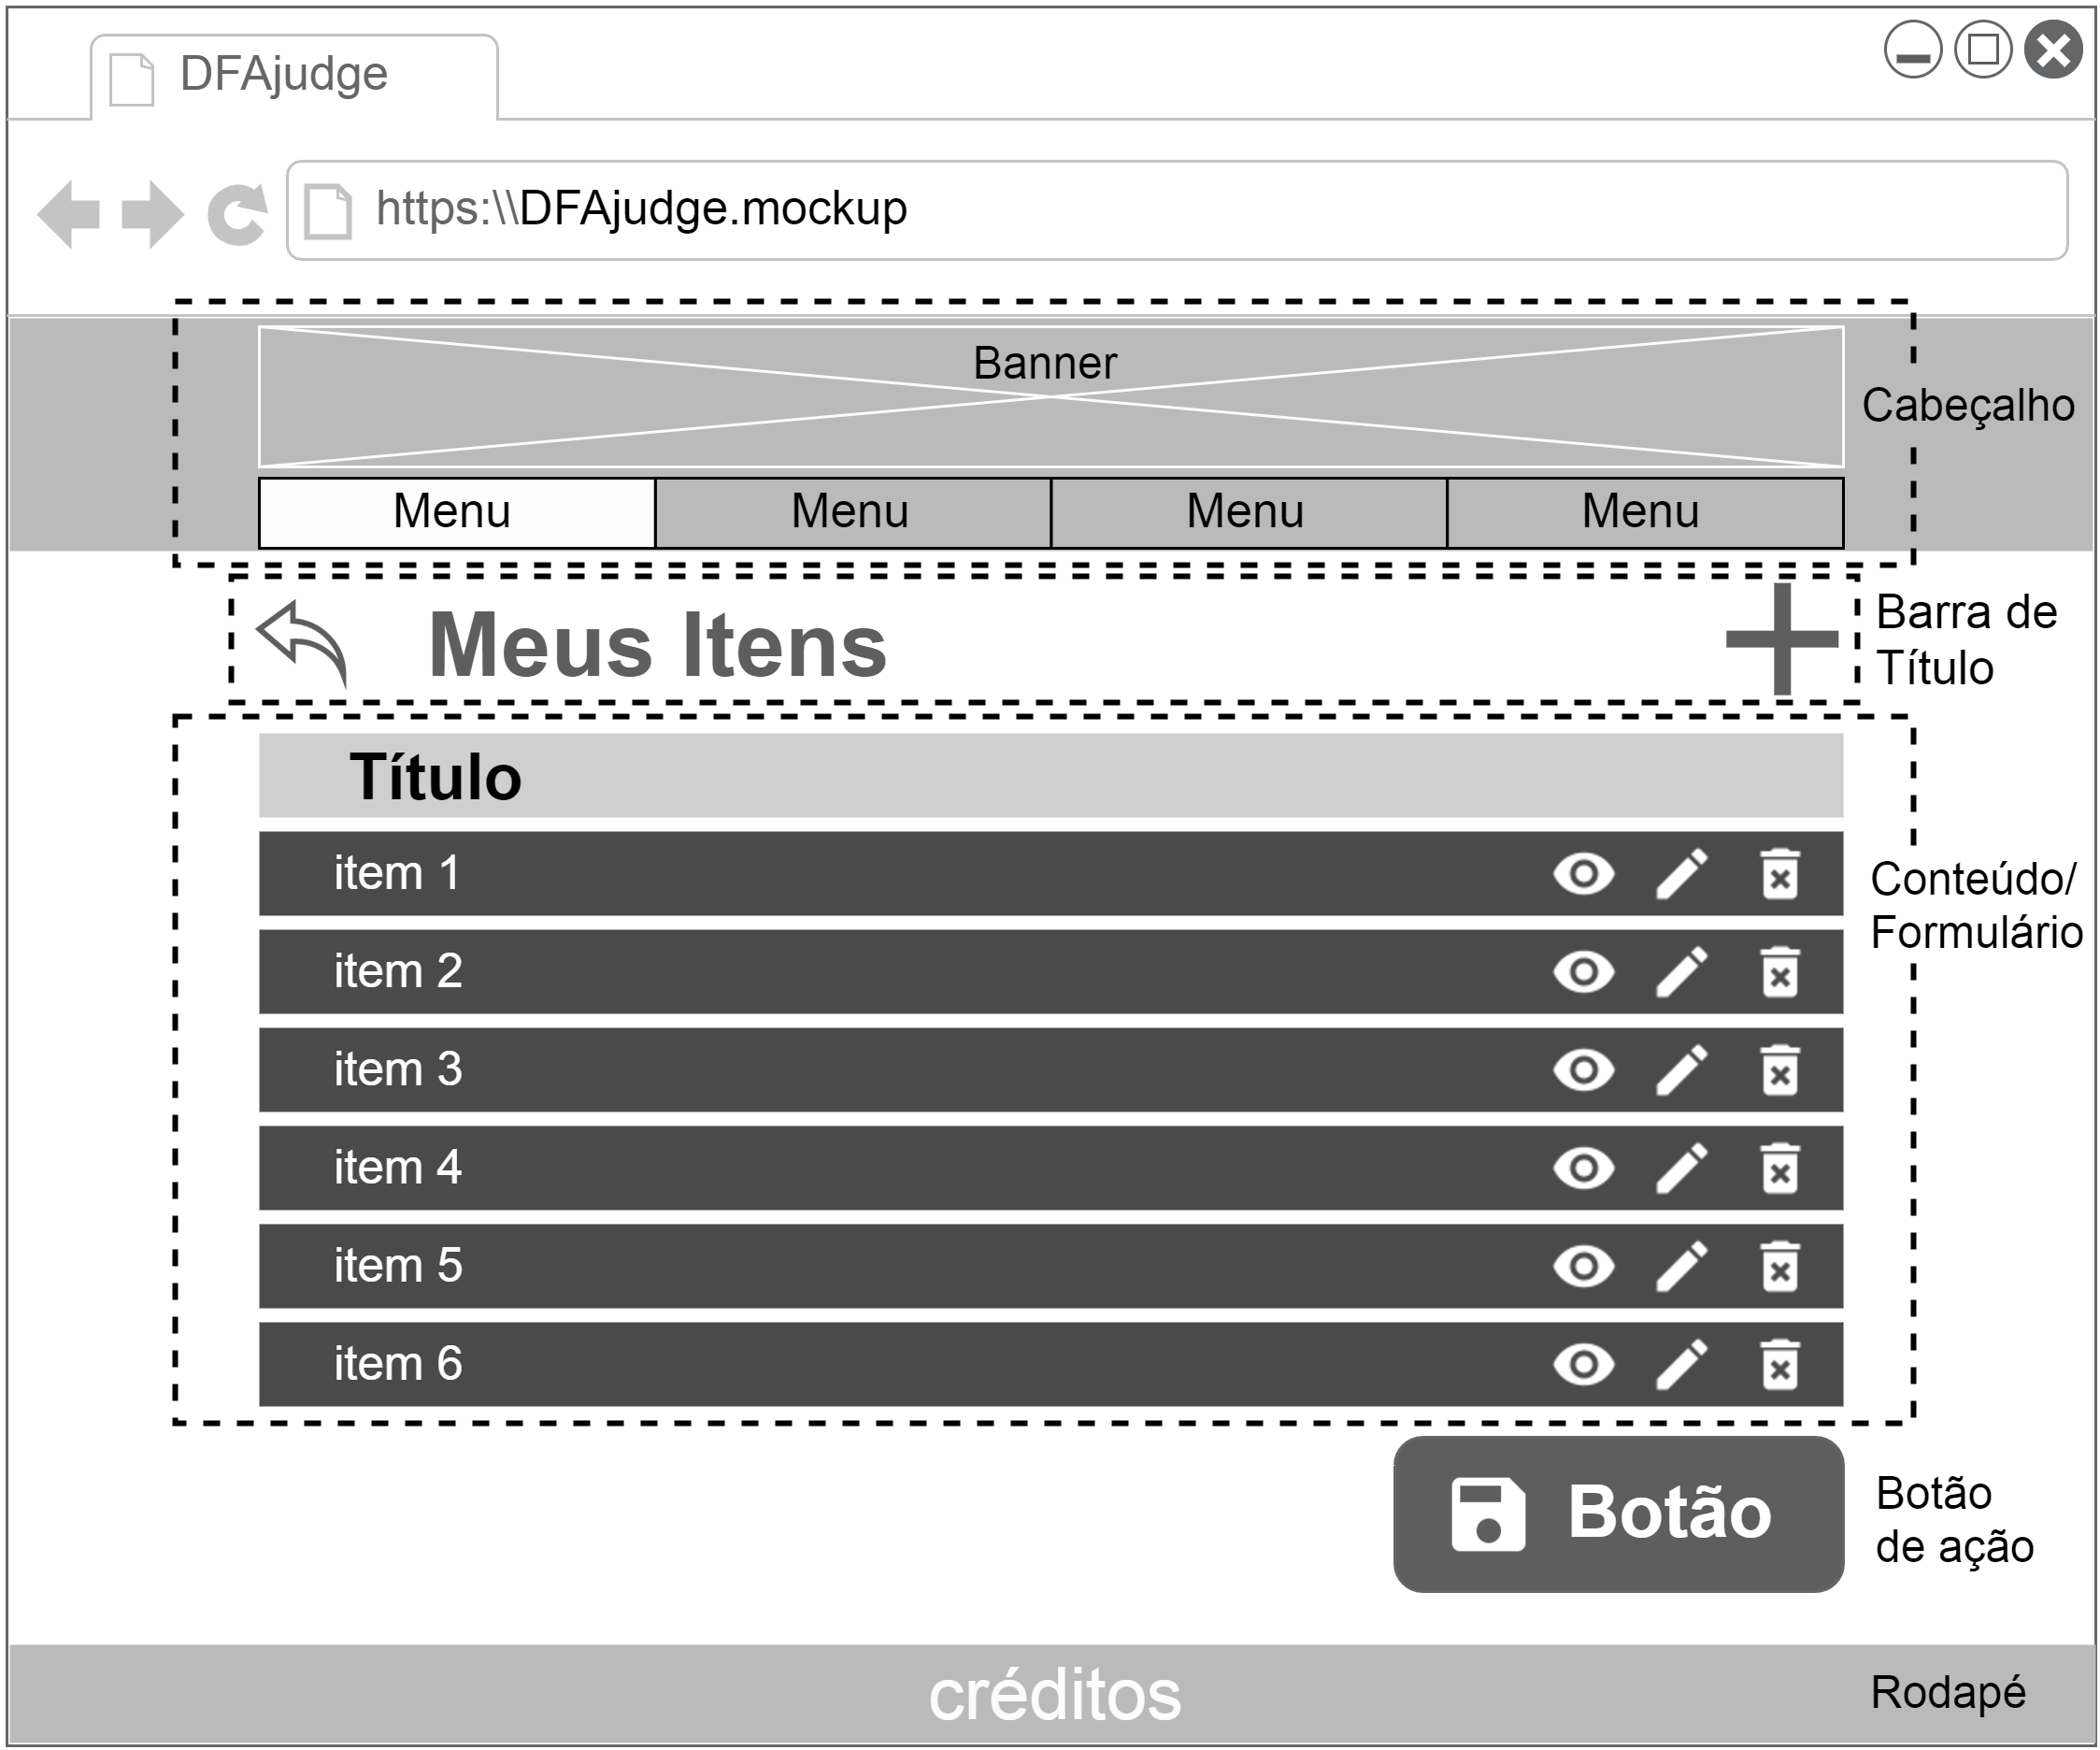
\includegraphics[width=\textwidth]{mockupGerenciamento.png}%[scale=0.2]
  \caption{Mockup do gerenciamento.}
  \label{fig:MockupGerenciamento}
  \vspace{-0.5cm}
\end{figure}

  A Figura~\ref{fig:MockupGerenciamento} exemplifica a interface que gerencia os itens das entidades: Turmas, Listas, Questões ou Usuários. No cabeçalho há um banner e um menu de navegação. Em seguida há uma barra com o título da interface e botões de ação pertinentes àquela página. Abaixo, são listado todos os itens, e em cada linha há botões de ação referentes àquele item. Nesta mesma configuração, é possível, ao invés de listar dados, o sistema exibir um formulário para inserir ou editar algum item. %E por último, o rodapé.
  
\begin{figure}[H]
  \centering
  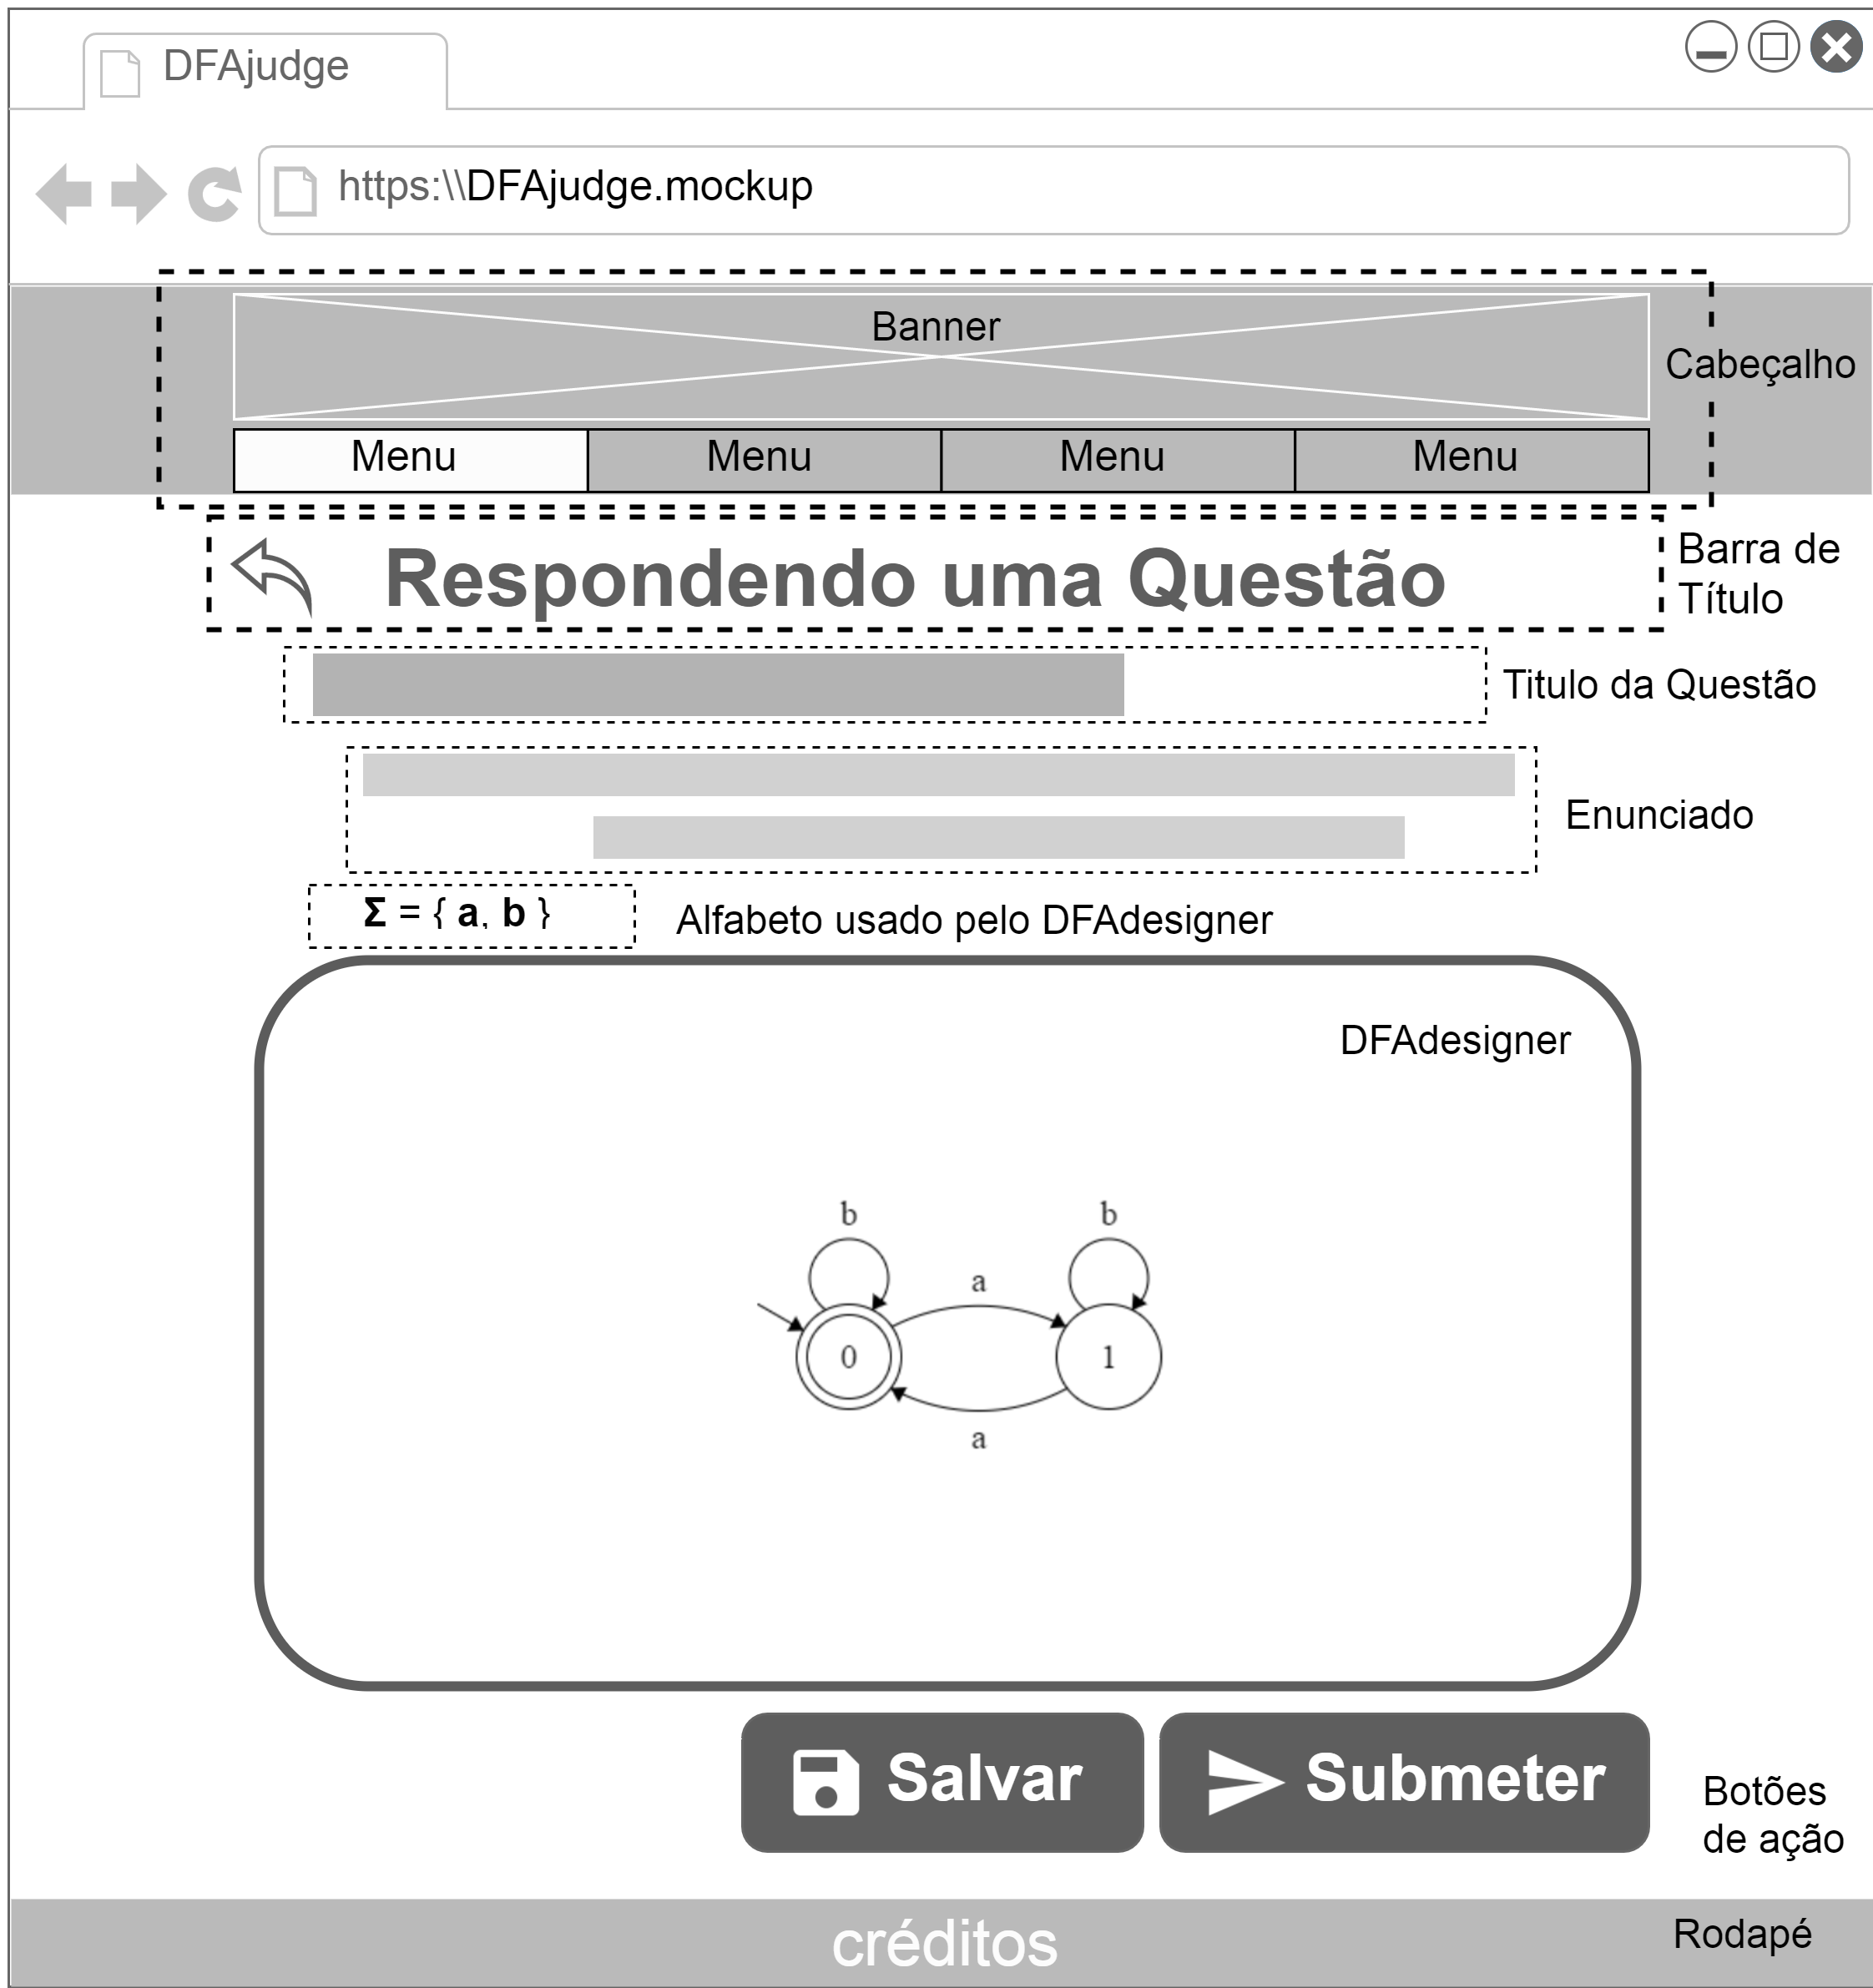
\includegraphics[width=\textwidth]{mockupDFAdesigner.png}%[scale=0.2]
  \caption{Mockup do formulário de resposta.}
  \label{fig:mockupDFAdesigner}
  \vspace{-0.5cm}
\end{figure}

  A Figura~\ref{fig:mockupDFAdesigner} exemplifica a interface que o aluno utilizará para resolver uma questão. Este formulário contém: o título da questão e o seu enunciado, o conjunto de símbolos do alfabeto desta questão, o DFAdesigner para confeccionar o seu autômato-resposta e ao final os botões de Salvar e de Submeter. Este \textit{mockup} serviu como base para todas as outras interfaces que o sistema possui. Seguido este modelo, pudemos garantir uma padronização que resultou em uma melhor usabilidade do sistema, que discutiremos nos capítulos seguintes.

% \section {ESPECIFICAÇÃO DE TESTES}
%   \subsection {cx preta}
%   \subsection {cx branca ( e fluxo do algoritmo )}
% \section {ANÁLISE DE PONTOS DE FUNÇÃO}
%   \subsection {Memorial de Cálculo}
%   \subsection {Fatores de Complexidade}
%   \subsection {Fatores de Ajuste}
%   \subsection {Análise de Pontos de Função}
% \section {Checklist}

\chapter[O sistema DFAjudge] {O sistema DFAjudge}

  Neste capitulo será mostrado o resultado final do desenvolvimento deste sistema. A este sistema foi atribuído o nome de \textbf{DFAjudge}, abreviação de \textit{Deterministic Finite Automata Judge}, ou em português, Juiz dos Autômatos Finitos Determinísticos. O logo do DFAjudge pode ser visto abaixo, ele é constituído de um autômato de um único estado, que é o inicial e de aceitação, e a partir dele há uma transição para ele mesmo sobre o simbolo ``judge''. Simbolizando que o estado é o autômato-resposta por você confeccionado, que ao submete-lo ao Juiz, ele o retorna aceitando-o. %, conforme o seu veredicto. %$DFA_{judge}$
  
\begin{figure}[H]
  \centering
  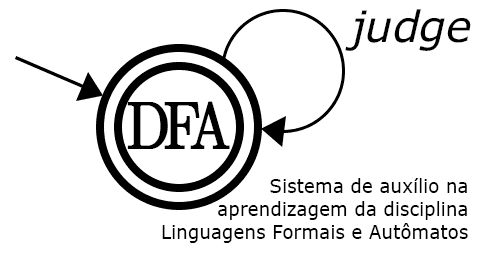
\includegraphics[scale=0.6]{prints/logo.png}
  \caption{Logo do DFAjudge.}
  \label{fig:logoDFAjudge}
  \vspace{-0.5cm}
\end{figure}
    
  A partir de agora veremos alguns \textit{screenshots} do DFAjudge, em escala reduzida, e acompanhados de comentários sobre detalhes omitidos nas seções anteriores. Com o apoio da Figura~\ref{fig:fluxoTelas} o usuário poderá ver onde ocorre as ações que interligam as páginas. Começamos pela tela de Login. 
  
\begin{figure}[H]
  \centering
  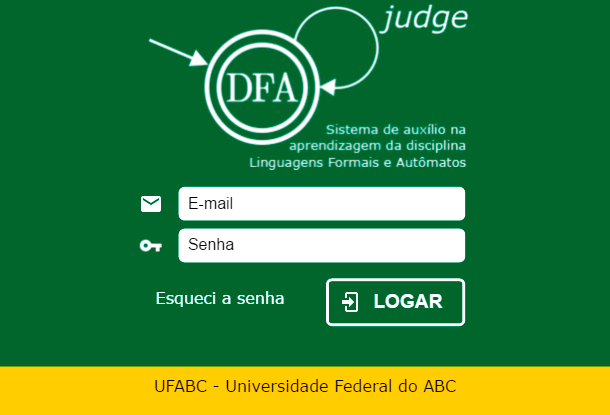
\includegraphics[scale=0.5]{prints/login.png}
  \caption{Login.}
  \label{print:login}
  \vspace{-0.5cm}
\end{figure}

  Neste formulário de login é necessário inserir o e-mail e senha para o usuário ter acesso ao sistema. Há também a possibilidade de recuperar a senha, caso esquecida, como vemos na Figura~\ref{print:resetNovaSenha}.


\begin{figure}[H]
  \centering
  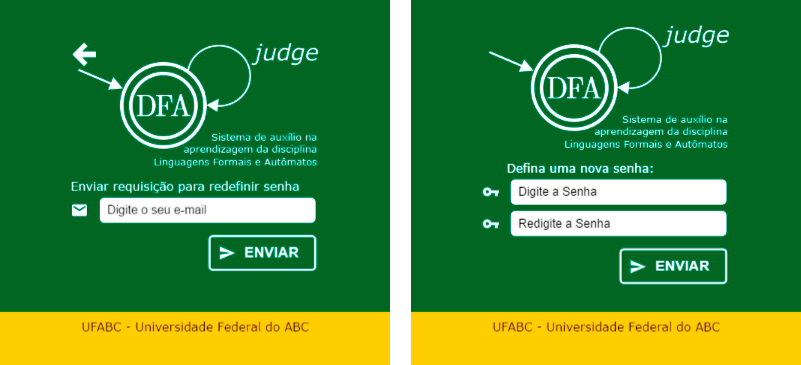
\includegraphics[width=\textwidth]{prints/resetnovaSenha.png}
  \caption{Tela de Requisição e Definição de Nova Senha.}
  \label{print:resetNovaSenha}
  \vspace{-0.5cm}
\end{figure}

  A tela a esquerda é a de Requisição de Redefinição de Senha, e ela é acessível pela tela de Login para onde é possível retornar através do link representado pela seta na área superior. Neste formulário é necessário que o usuário digite um e-mail cadastrado no sistema para ser enviado, neste mesmo e-mail, o link de acesso à tela de Definir Nova Senha, que está a direita na figura, onde o usuário deve digitar sua nova senha e redigita-la abaixo.
  
  Um detalhe importante é que, logicamente, para requisitar a redefinição de sua senha, o usuário deve inserir seu e-mail que está de fato cadastrado no sistema. Mas no caso de um usuário mal intencionado, tentar inserir e-mails aleatórios afim de descobrir qual realmente consta no sistema, esta tela se torna porta de entrada para outros tipos de ataques, visto que agora possui o conhecimento de que tal usuário está de fato cadastrado no sistema. Por isto, quando o usuário enviar uma requisição, apenas é exibida a mensagem: ``E-mail enviado com sucesso! Cheque seu e-mail''. Deste modo, cadastrado ou não o e-mail, o atacante não receberá uma \textit{feedback} conclusivo sobre sua tentativa.

  Como visto anteriormente, o sistema envia e-mails aos usuários em ocasiões especificas. No total são 3 tipos de e-mails, que podemos ver na Figura~\ref{print:emails}. O primeiro e-mail é enviado quando o usuário é adicionado no sistema, tanto na interface do professor de adicionar novos usuários ou de adicionar alunos em lote em uma Turma, neste e-mail há uma mensagem de boas vindas e instruções de como definir uma nova senha na segunda tela vista na Figura~\ref{print:resetNovaSenha}. A segunda mensagem diz ao usuário que sua requisição de alteração de senha foi feita, pelo formulário de Requisição de Redefinição de Senha da figura anterior, e abaixo está o link para a tela de Definição de Nova Senha. Uma particularidade deste link é que contém um \textit{token} que assegura que esta definição de senha é unicamente para aquele usuário, e seu valor foi formado por uma \textit{hash} do horário em microssegundos que foi feita aquela requisição. A terceira mensagem se trata de um alerta que sua senha de acesso foi alterada, afim de avisar o usuário que a operação foi concluída com sucesso.

\begin{figure}[H]
  \centering
  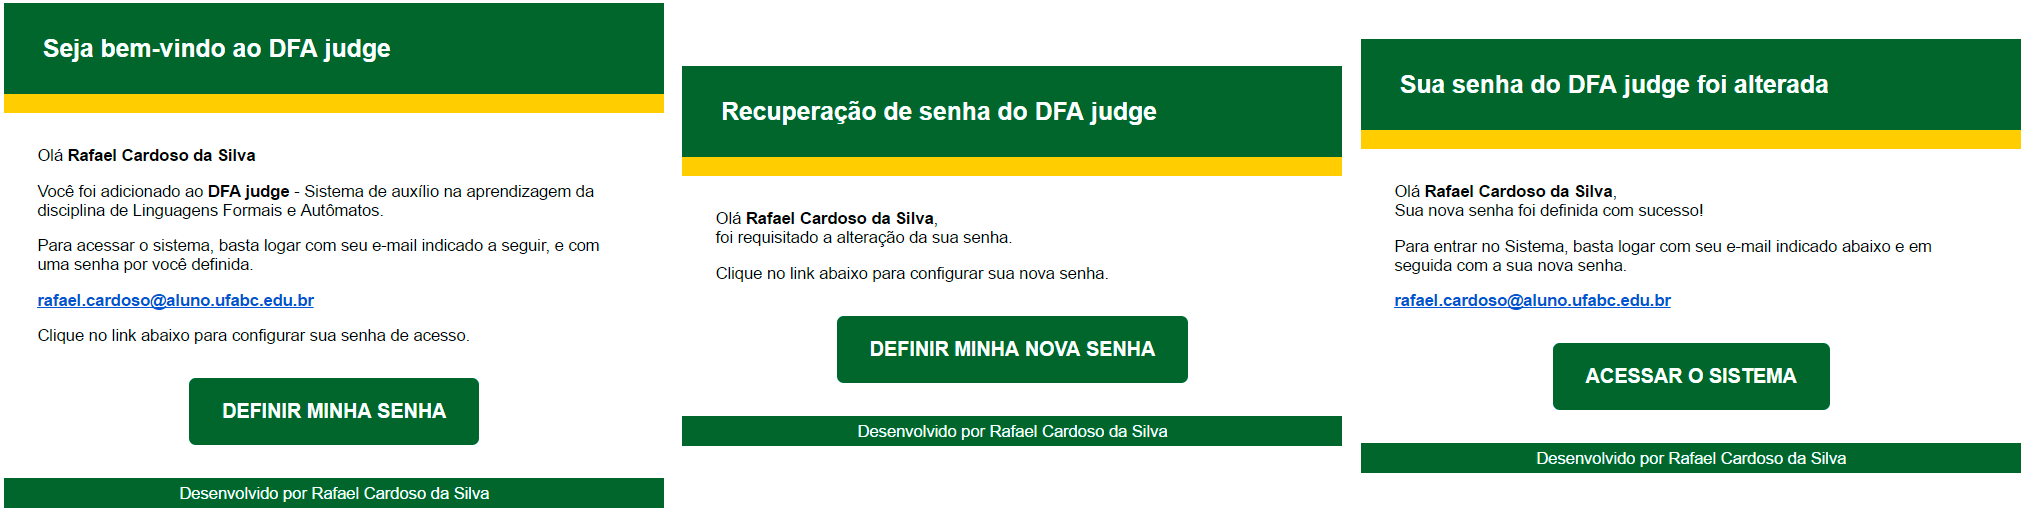
\includegraphics[width=\textwidth]{prints/emails.png}
  \caption{Mensagens de e-mail que o sistema envia.}
  \label{print:emails}
  \vspace{-0.5cm}
\end{figure}

  Após o usuário logar no sistema, ele é redirecionado para a Home, como podemos ver na figura a baixo, na qual se trata da Home do usuário Professor.
  
\begin{figure}[H]
  \centering
  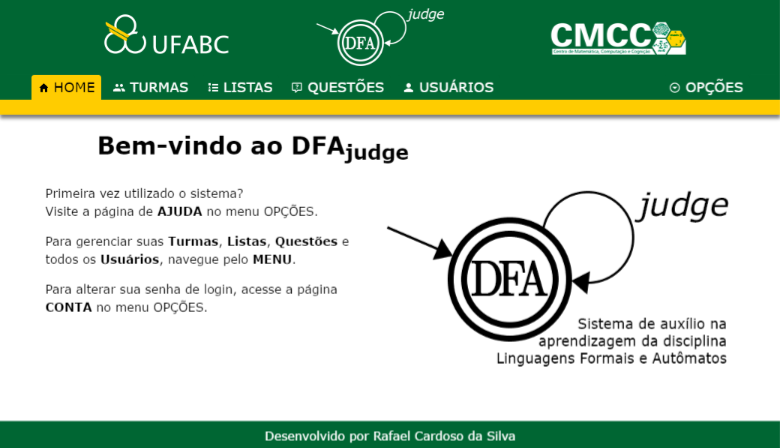
\includegraphics[width=\textwidth]{prints/profHome.png}
  \caption{Home do Professor.}
  \label{print:profHome}
  \vspace{-0.5cm}
\end{figure}

  Nesta tela podemos observar a interface padrão do sistema, onde no cabeçalha há um banner com os logos da UFABC, do DFAjudge e do CMCC. Logo abaixo há o menu de navegação, que logo detalharemos. Ao centro há o conteúdo da página, que é especifico em cada interface. E ao final está o rodapé com os créditos do desenvolvimento.
  
   O conteúdo da página Home é semelhante para os dois usuários, nele há o logo do DFAjudge e a esquerda há indicações para os usuários, sobre onde se encontra a Ajuda e como navegar pelo sistema, e no caso do aluno, para ele se atentar a data limite de submissão.

   %A figura a seguir mostra a diferença entre o menu do Professor e do Aluno.
    
  %\includegraphics[width=\textwidth]{prints/menus.png}
  %\caption{Menu do Professor acima e do Aluno abaixo.}
  %\label{print:menu}

  
  O Menu de Navegação é distinto para cada usuário e apresenta configurações diferentes dependendo do contexto. Abaixo vemos todas as possíveis interações do menu para o usuário Professor.
  
\begin{figure}[H]
  \centering
  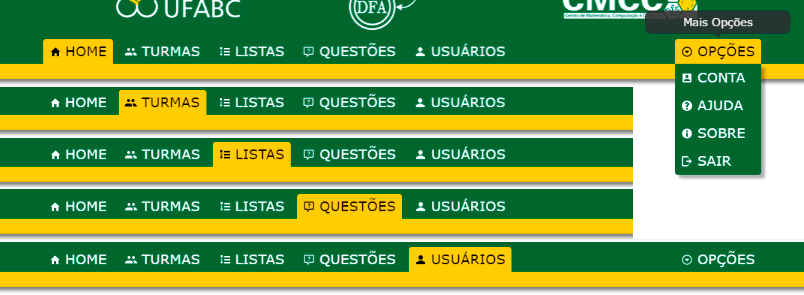
\includegraphics[width=\textwidth]{prints/menuProf.png}
  \caption{Colagem do Menu do Professor.}
  \label{print:menuProf}
  \vspace{-0.5cm}
\end{figure} 
     
  O Professor tem acesso a todos os itens criados por ele, que são: as questões, as listas com suas questões, as turmas com alunos e suas listas, e também acesso a todos os usuários do sistema. Assim, conforme a página que o professor visualizar, o menu se comporta de modo diferente, ou seja, ele destaca qual dos itens do menu que se relaciona com o conteúdo. Por exemplo, se ele estiver visualizando uma turma, o item Turmas estará em destaque, já se ele estiver editando uma questão, o item Questões se destacará.
  
  Já o usuário do tipo Aluno, tem seu acesso de modo linear, ou seja, ele seleciona primeiramente a sua turma, depois abre uma lista, em seguida escolhe uma questão, e ao fim responde esta questão. Então o menu também se comporta seguindo o contexto, como podemos ver na figura abaixo.
  
\begin{figure}[H]
  \centering
  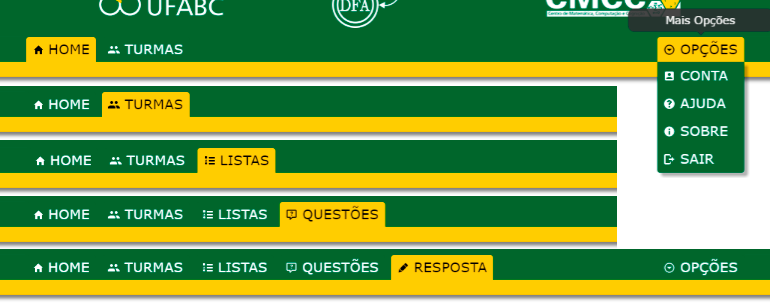
\includegraphics[width=\textwidth]{prints/menuAluno.png}
  \caption{Colagem do Menu do Aluno.}
  \label{print:menuAluno}
  \vspace{-0.5cm}
\end{figure}

  Mas diferente do professor, os itens do menu do Aluno vão sendo adicionado conforme ele se aprofunda no acesso, visto a dependência entre as entidades, ou seja, não poderia acessar uma lista de questões sem antes selecionar a sua turma e uma lista. Também deste modo, o menu oferece um rápido regresso entre os itens, não sendo necessário voltar uma a uma.
  
  O item Opções do menu oferece aos dois usuários algumas ações, como: Conta, Ajuda, Sobre e Sair do sistema. Na tela Conta, é possível visualizar dados de sua conta e também redefinir sua senha pessoal como vemos na Figura~\ref{print:conta}.
   
\begin{figure}[H]
  \centering
  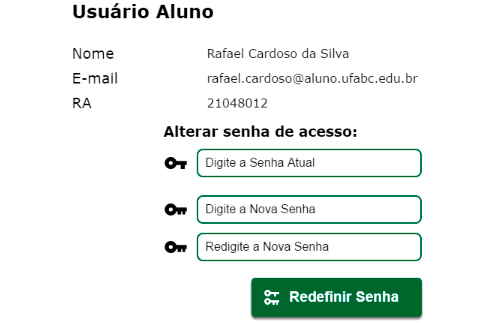
\includegraphics[width=0.7\textwidth]{prints/conta.png}
  \caption{Tela da Conta do usuário.}
  \label{print:conta}
  \vspace{-0.5cm}
\end{figure}
  
  Já na tela de Ajuda, que podemos ver na Figura~\ref{print:ajuda}, há um tutorial que utiliza animações e texto para ensinar o usuário a utilizar o DFAdesigner e outros recursos do sistema, como a interpretação das mensagens de \textit{feedback} ou mensagens de erro na construção de seu autômato-resposta. Cada animação demonstra muito bem as ações que devem ser tomadas para realizar certa interação. Para fazer as animações foram utilizadas capturas de tela e ícones que ajudam a representar as ações realizadas. Além disso, há um texto descritivo ao lado de cada desta animação, afim de melhor detalha-la. %Na Figura~\ref{print:ajuda} podemos visualizar o começo do conteúdo desta página.
     
\begin{figure}[H]
  \centering
  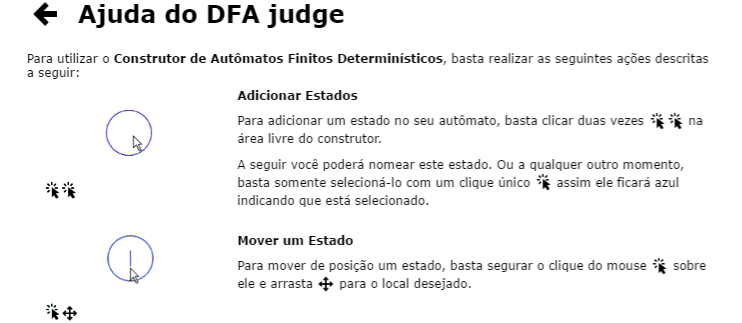
\includegraphics[width=\textwidth]{prints/ajuda.png}
  \caption{Conteúdo da tela de Ajuda.}
  \vspace{-0.2cm}
  \label{print:ajuda}
  \vspace{-0.5cm}
\end{figure}
    
  O Professor desempenha um papel fundamental no sistema, ele deve gerenciar tudo. A seguir veremos o conteúdo de algumas telas que o professor utiliza.
  
  Na Figura~\ref{print:profQuestoes} são listados as Questões do Professor, por meio de uma lista, em que cada item exibe o título da questão e botões de ação, como: visualizar, editar, duplicar e remover esta questão. A ação de duplicar uma questão foi uma sugestão do próprio orientador durante testes do sistema, em que ele sentiu a necessidade de facilitar a criação de questões que possuam semelhanças, ou seja, quando confeccionar uma questão semelhante a outra já criada, mas que difere em poucos detalhes, é mais fácil poder duplicar-la e modifica-la, do que confecciona-la do zero. Demonstrando assim que teste de usabilidade do sistema com usuários de verdade resultam em funcionalidade não antes consideradas. 
  
  Outra funcionalidade é a possibilidade do professor importar e exportar suas questões em formato JSON, que é muito útil para fazer \textit{backups}, e esta tela é acessível pelo link com ícone de \textit{upload} e de \textit{download} na barra de título desta tela.
        
\begin{figure}[H]
  \centering
  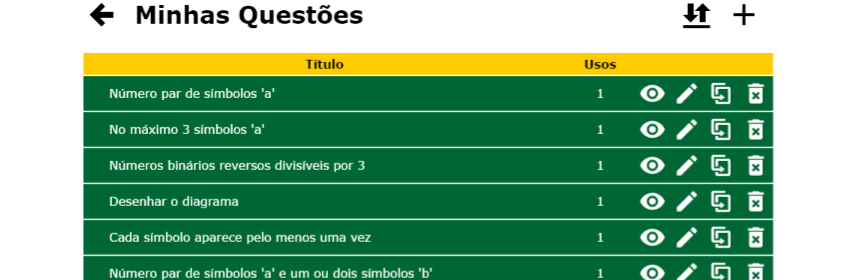
\includegraphics[width=\textwidth]{prints/profQuestoes.png}
  \caption{Lista de Questões de uma Lista.}
  \label{print:profQuestoes}
  \vspace{-0.5cm}
\end{figure}

  Como o gerenciamento das Turmas, das Listas, das Questões e dos Usuário tem sua interface muito semelhantes, então não apresentaremos elas aqui, pois assim teremos mais oportunidade de explorar outros detalhes mais relevantes.
  
  A Figura~\ref{print:profEditarQuestao} a seguir, apresenta o formulário para editar e criar uma nova questão. No primeiro campo deve-se inserir título da questão. No campo do corpo é redigido o enunciado da questão. Tanto no título, quanto no corpo é possível utilizar marcações de comando \LaTeX\xspace e elementos HTML. Assim ao editar o corpo da questão, logo abaixo na área de borda amarela é exibido o resultado final do enunciado. Em seguida são inseridos os símbolos do conjunto $\Sigma$, cada um separado por um espaço, pois este conjunto é utilizado posteriormente pelo DFAdesigner e pelo Juiz. 
  
  Em seguida está o DFAdesigner, no qual o professor pode confeccionar o autômato-gabarito. A área ocupada pelo DFAdedigner é grande, o que proporciona criar autômatos de diversos tamanhos e de forma mais espaçosa. Então, após criada a questão, basta clicar no botão de Salvar, caso esteja editando, ou Inserir, caso seja uma nova questão. Em seguida o professor é direcionado para a tela de Visualizar Questão, onde a questão é exibida da forma que apareceria para o aluno, como vemos posteriormente na Figura~\ref{print:alunoResposta}.
 
  %E logo abaixo está o DFAdesigner, na qual pelo motivo de seu tamanha, na figura ele ouve uma compacta
  %Obs: A altura do DFA designer foi editado afim de contemplar todo o formulário em uma \textit{screenshot} mais compacta.

\begin{figure}[H]
  \centering
  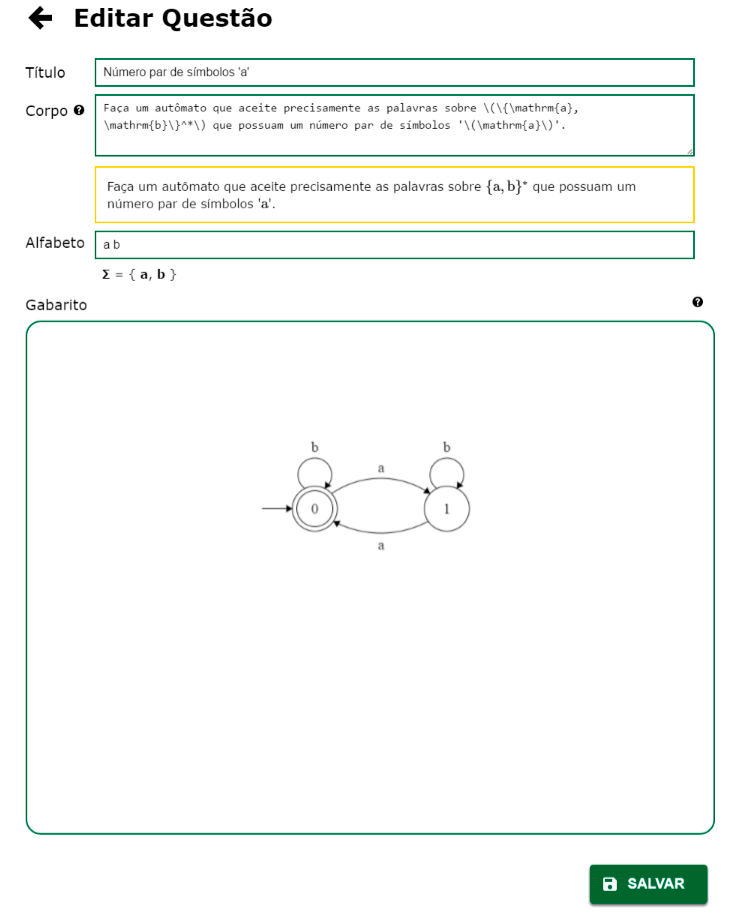
\includegraphics[width=0.9\textwidth]{prints/profEditarQuestao.png}
  \caption{Formulário de Criação ou Edição de Questão.}
  \label{print:profEditarQuestao}
  \vspace{-0.5cm}
\end{figure}

  Todas as telas, que editam ou criam um novo item, são as mesmas páginas, como vimos na Figura~\ref{fig:fluxoTelas}. Porém, se caso for uma edição, então os campos do fomulário estarão preenchidos com os antigos dados, senão estará em branco, caso for um novo item.
  
  %Em todas as telas utilizadas para editar ou criar um novo item, como visto pelo diagrama de Fluxo de Telas na Figura~\ref{fig:fluxoTelas}, são as mesmas páginas. Porém no caso de editar, os dados anteriormente salvo estão já preenchendo o formulário. Senão, no caso de um novo item, o formulário estará vazio.

  Na Figura~\ref{print:profListaDeQuestoes} vemos a relação das questões presentes em uma lista, e também o título e a contagem de questões desta lista. Nesta tela é possível acessar a tela de edição desta lista clicando no ícone de lápis no canto superior direito. Também é possível, através do ícone ao lado, ir para a tela de ordenação de questões, onde com o clicar e arrastar do mouse pode-se reordenar as posições das questões na lista.

\begin{figure}[H]
  \centering
  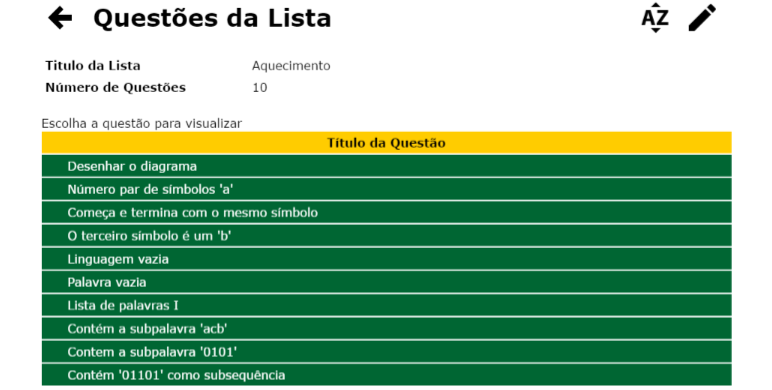
\includegraphics[width=\textwidth]{prints/profListaDeQuestoes.png}
  \caption{Lista de Questões de uma Lista.}
  \label{print:profListaDeQuestoes}
  \vspace{-0.5cm}
\end{figure}

  Na Figura~\ref{print:profEditarLista} vemos a tela de Editar Lista, onde temos o campo para inserir um título para esta lista e a relação de todas as questões deste professor, para que ele possa selecionar quais irão compor a lista. A coluna Usos também foi uma sugestão dada pelo orientador durante a implementação, para mostrar quais questões ainda não tinham sido adicionada em uma lista.

\begin{figure}[H]
  \centering
  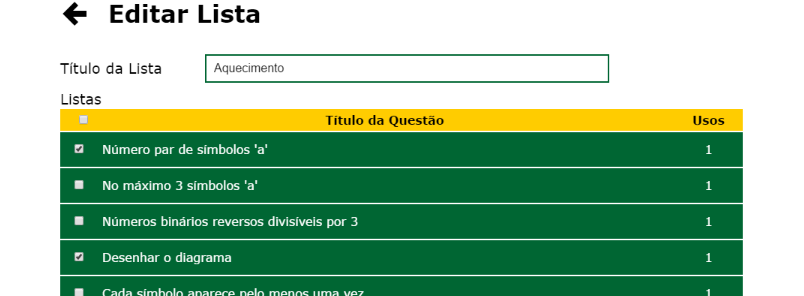
\includegraphics[width=\textwidth]{prints/profEditarLista.png}
  \caption{Editar Lista de Questões.}
  \label{print:profEditarLista}
  \vspace{-0.5cm}
\end{figure}

  Na Figura~\ref{print:profTurmaDetalhes} vemos os detalhes de uma turma. Nesta tela está listada todos os alunos da turma e todas as listas aplicadas a ela, onde podemos alternar a visualização destas duas por meio de abas. Nesta tela é possível também acessar a edição desta turma, que é semelhante às das Listas, onde nela são relacionadas todas suas listas e alunos para serem selecionados afim de compor a turma. A partir do Detalhes da Turma pode-se acessar o relatório de desempenho desta turma, pelo ícone que representa uma tabela.

\begin{figure}[H]
  \centering
  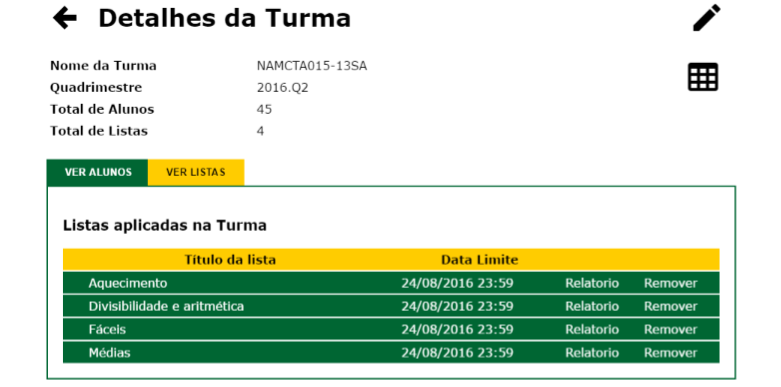
\includegraphics[width=\textwidth]{prints/profTurmaDetalhes.png}
  \caption{Detalhes de uma Turma.}
  \label{print:profTurmaDetalhes}
  \vspace{-0.5cm}
\end{figure}

  Na Figura~\ref{print:profRelatorioTurma} vemos um exemplo do relatório de desemprenho de uma turma, onde as linhas correspondem aos alunos matriculados e as colunas correspondem às listas aplicadas àquela turma. Cada posição da tabela possui a contagem de acertos que cada aluno obteve em cada lista e, na ultima coluna, está o total de acertos e a porcentagem correspondente. Nesta tela também há a possibilidade de exportar esta tabela em formato CSV, afim de utiliza-la em uma planilha eletrônica para ajudar a compor a nota de cada aluno.
  
\begin{figure}[H]
  \centering
  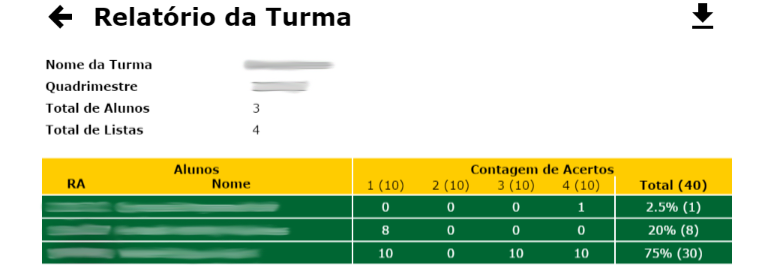
\includegraphics[width=\textwidth]{prints/profRelatorioTurma.png}
  \caption{Relatório de uma Turma.}
  \label{print:profRelatorioTurma}
  \vspace{-0.5cm}
\end{figure} 

  A partir de agora falaremos das telas com as quais o usuário do tipo Aluno interage. Após o login, o aluno se depara com uma tela igual à Home do Professor. Em seguida, ao clicar em Turmas no Menu, ele é redirecionado para a tela da Figura~\ref{print:alunoTurmas}, onde deve clicar sobre sua turma.
  
\begin{figure}[H]
  \centering
  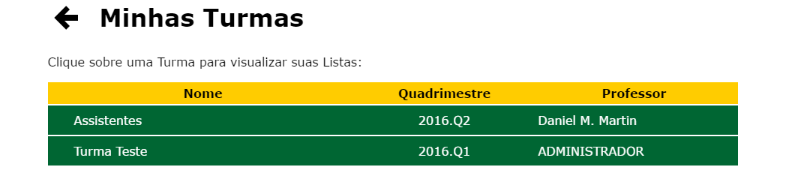
\includegraphics[width=\textwidth]{prints/alunoTurmas.png}
  \caption{Turmas do Aluno.}
  \label{print:alunoTurmas}
  \vspace{-0.5cm}
\end{figure}

  Na Figura~\ref{print:alunoListas} vemos todas as lista aplicadas na turma do Aluno. Primeiramente é exibido o nome daquela turma, o quadrimestre em que está sendo ofertada e o professor que criou esta turma. Logo abaixo são listadas as Listas aplicadas a ela. Onde, em cada item, encontra-se o título, a data limite para submissão de resposta e ,na última coluna, o número de acertos do total de questões.

\begin{figure}[H]
  \centering
  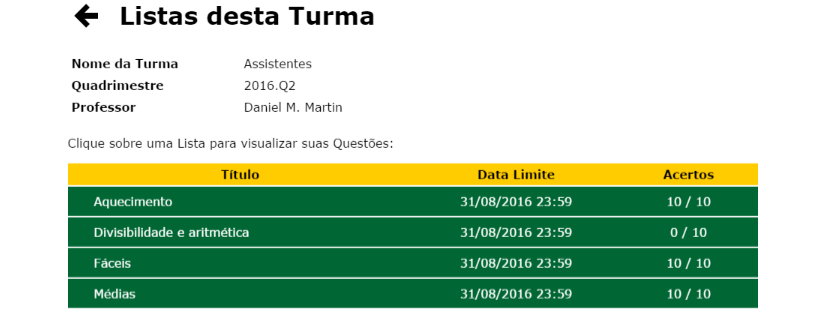
\includegraphics[width=\textwidth]{prints/alunoListas.png}
  \caption{Listas do Turma do Aluno.}
  \label{print:alunoListas}
  \vspace{-0.5cm}
\end{figure}
  
  Ao selecionar um item da Lista, veremos a tela da Figura~\ref{print:alunoQuestoes}, que são as questões daquela lista. Temos novamente o nome daquela turma, o quadrimestre, o professor e, agora, informações sobre aquela lista: seu nome, a sua data limite de entrega e a contagem de acertos. Abaixo estão listadas todas as questões daquela lista, onde em cada item temos o título da questão e, na direita, um ícone para simbolizar o seu status. No exemplo da figura, na primeira questão o aluno acertou a resposta, na segunda ele salvou como rascunho, na terceira sua resposta está incorreta e nas outras, sem ícones, ele simplesmente não as respondeu.
  
  Um detalhe importante é que as listas têm data limite de entrega. Assim, caso o aluno tenha ultrapassado esta data, nesta tela e também na anterior haverá um ícone de atenção e uma mensagem dizendo que o prazo para submeter as respostas acabaram, e não será possível submeter e nem salvar. Outro detalhe é que mesmo com a data de tolerância passada, o Aluno poderá acessar todas as questões e somente visualizar suas respostas, afim de poder estudar para a prova.

\begin{figure}[H]
  \centering
  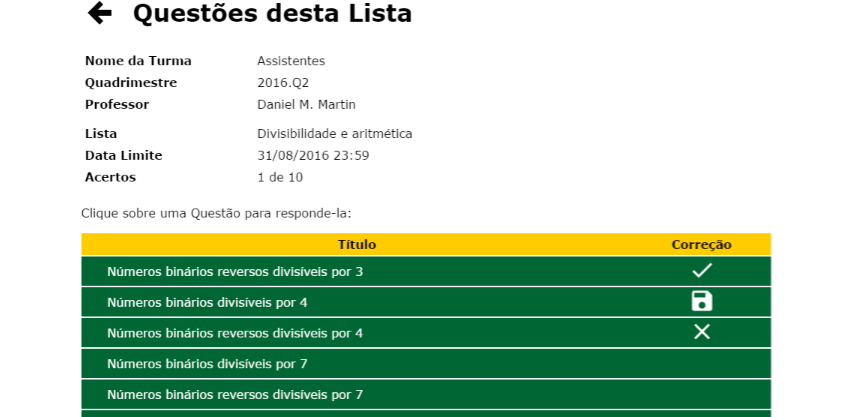
\includegraphics[width=\textwidth]{prints/alunoQuestoes.png}
  \caption{Questões daquela Lista.}
  \label{print:alunoQuestoes}
  \vspace{-0.5cm}
\end{figure}

  Ao selecionar uma questão para resolve-la, a tela da Figura~\ref{print:alunoResposta} é exibida. Nela, é possível interagir com o DFAdesigner para confeccionar o autômato-resposta para aquela questão e depois submete-lo ao Juiz.%, para assim receber, logo abaixo, o seu veredicto.

\begin{figure}[H]
  \centering
  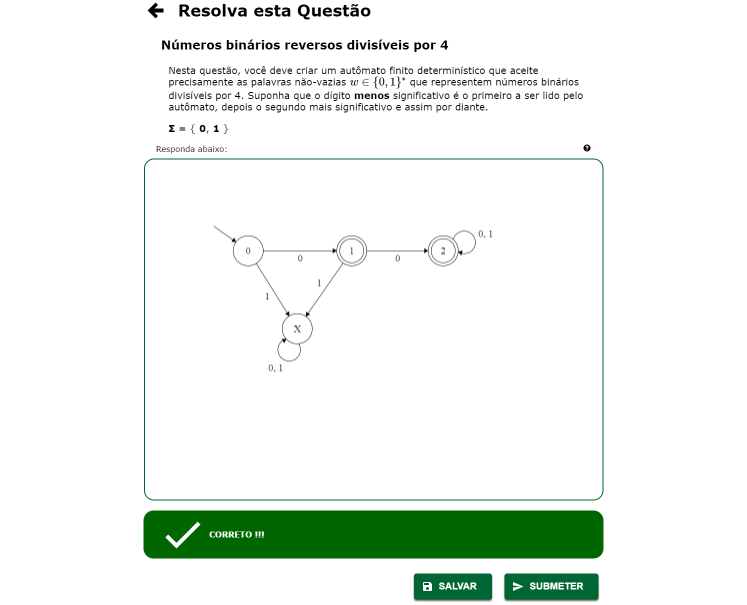
\includegraphics[width=\textwidth]{prints/alunoResposta.png}
  \caption{Aluno respondendo uma questão.}
  \label{print:alunoResposta}
  \vspace{-0.5cm}
\end{figure}

  Como podermos observar na Figura~\ref{print:alunoResposta}, o veredicto do Juiz é exibido logo abaixo do DFAdesigner. Então todos os possíveis veredictos do Juiz e também a mensagem que alerta sobre a data limita, estão na colagem da figura a seguir. No caso da resposta ser incorreta, o \textit{feedback} do juiz será acompanhado da palavra que o distinguiu, como uma dica para o Aluno entender o que ele errou em seu autômato-resposta.

\begin{figure}[H]
  \centering
  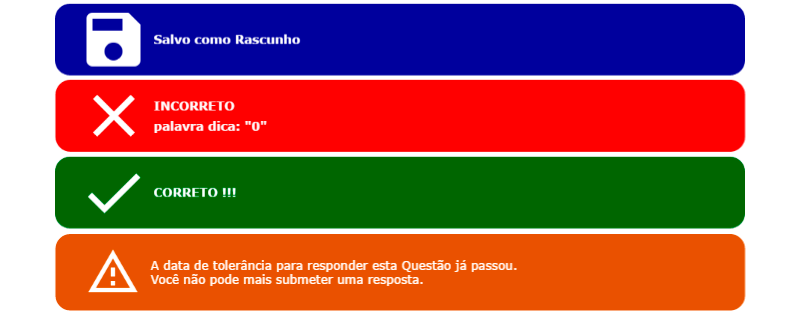
\includegraphics[width=\textwidth]{prints/alunoFeedback.png}
  \caption{Colagem do \textit{feedback} da resposta.}
  \label{print:alunoFeedback}
  \vspace{-0.5cm}
\end{figure}
    
  Antes de submeter a resposta ao Juiz, o DFAdesigner realiza uma verificação no diagrama construído, e se houver algum erro, próximo ao \textit{feedback}, será exibido os erros cometidos pelo aluno na confecção do autômato, como vemos no exemplo a seguir.
  
\begin{figure}[H]
  \centering
  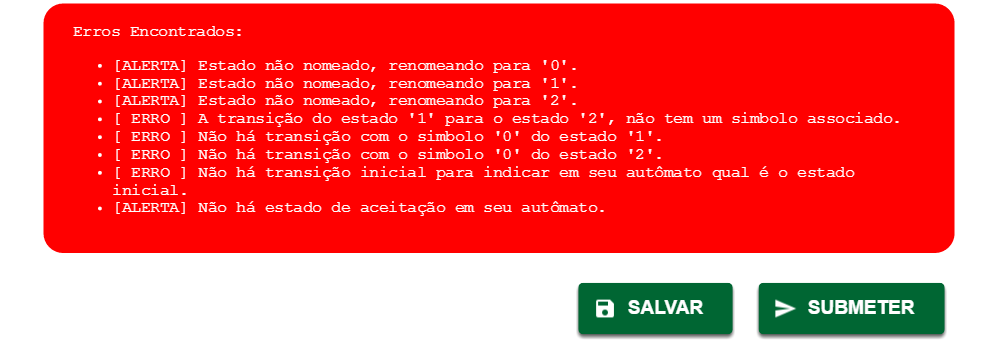
\includegraphics[width=\textwidth]{prints/alunoErros.png}
  \caption{Erros na construção do autômato-resposta.}
  \label{print:alunoErros}
  \vspace{-0.5cm}
\end{figure}

  São listados dois tipos de mensagens: Alerta e Erro. O alerta não influência na correta construção do AFD, mas o erro sim. Neste exemplo, o aluno é alertado de que há estados não nomeados e de que estes foram nomeados com números automaticamente. Mas não é necessário os estados terem nomes, porém como eles nomeados ficará mais fácil descrever os outros erros para o usuário. Em seguida são listados erros críticos sobre a construção de um AFD, como: uma transição sem simbolo associado, a falta de transições a partir de um estado e que não foi demarcado o estado inicial. Assim, havendo algum erro, a submissão é abortada e o aluno, ao ler estas mensagens, poderá corrigir os seus erros.



\section{Designer do DFAjudge}

  Nesta seção analisaremos algumas particularidades a respeito do \textit{designer} das interfaces do DFAjudge. O objetivo de todas interfaces é tornar a interação com o usuário mais o simples e eficaz possível. Então ela deve ser suficientemente clara para que o usuário reconheça facilmente a utilidade e o objetivo dela. Assim, durante o desenvolvimento desde sistema houve a preocupação de maximizar a usabilidade e a experiência do usuário ao utilizar o sistema quando finalizado.
  
  Para começar, o esquema de cores utilizado na interface do DFAjudge, como já foi possível perceber, são as cores verde (\texttt{\#006633}) e o amarelo (\texttt{\#FFCC00}), pois além de serem as cores oficiais da UFABC, elas têm um ótimo constaste quando associamos o verde com branco e o amarelo com o preto. Assim, proporciona que certos elementos sejam destacados e ainda sejam suficientemente legível seu conteúdo na interface. %, e utilizaremos isso amplamente.
  
  Como vimos, a interface do aluno se sucede de maneira simples, onde ele realiza somente uma escolha por página. Desta maneira, os dados são exibidos de modo pregressivo e, consequentemente, evitando o excesso de informações exibidos ao aluno. Similarmente ocorre com o Professor, em que cada tela há somente um objetivo a ser realizado.
  
  %A interface do aluno se sucede de maneira simples, primeiro ele seleciona a sua turma, depois escolher uma lista e assim por diante, somente uma escolha por página. Pois desta maneira, são exibidas as informações de forma progressiva, referentes a esta escolha, assim evitando o excesso de informações para o aluno interpretar. Similarmente ocorre com o professor, em que cada tela tem um objetivo especifico, como por exemplo: somente listar suas questões, ou editar uma única lista, ou gerenciar sua turma.
  
  Como já falamos anteriormente, foi utilizado o artificio do menu se comportar de maneira dinâmica conforme o contexto da página, como vimos na Figura~\ref{print:menuProf} e na Figura~\ref{print:menuAluno}, e logo abaixo dele, para cada página, há uma barra de título, que nela tem primeiramente um link pra voltar para a página anterior (conforme vimos na Figura~\ref{fig:fluxoTelas}), um título simples, que ajuda a rapidamente identificar a página, e por último, links para outras páginas que realizam alguma ação sobre aquele objeto. A seguir vemos alguns exemplos de barras de título das páginas do professor.
 
\begin{figure}[H]
  \centering
  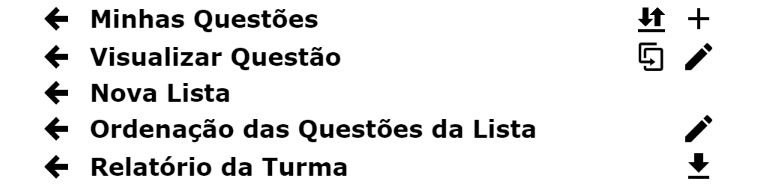
\includegraphics[width=0.9\textwidth]{prints/toolbar.png}
  \caption{Barra de título da página.}
  \label{print:toolbar}
  \vspace{-0.5cm}
\end{figure}

  Assim, a primeira impressão ao ler este título na barra, facilmente leva o usuário a reconhecer o objetivo daquela página, como no exemplo: listar minhas questões, visualizar uma questão, inserir uma nova lista, ordenar as questões de uma lista e exibir o relatório daquela turma. E o link de voltar em destaque na primeira posição, ajuda o usuário a facilmente retornar a página anterior àquela tela. E à direita, como se fossem opções extras, há links representados por imagens, que de forma intuitiva, oferece ao usuário a possibilidade de redireciona-lo para uma página que atue sobre aquele objeto, como: editar aquele item, inserir um novo item ou exportar aquela informação. 
  
  Então, a união do menu com esta barra, fornece ao usuário uma navegação mais rápida e de fácil identificação de sua localização. E todas as interfaces apresentam este mesmo padrão, resultando em uma boa usabilidade do sistema como um todo.
  
  Outro elemento presente em quase todas as páginas são os botões, como vemos na Figura~\ref{print:botoes}, eles são grandes de cor verde e com ícone e letras de cor branca, assim eles se destacam e o contraste entre as cores facilita a leitura. E também o efeito de sombra passa a sensação dele estar elevado, presumindo assim que são clicáveis. E a utilização de ícones ajuda na rápida interpretação da ação que o botão realiza. 
  
\begin{figure}[H]
  \centering
  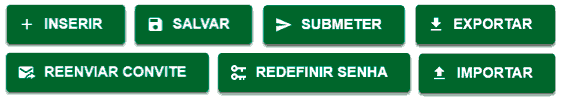
\includegraphics[width=\textwidth]{prints/botoes.png}
  \caption{Botões das interfaces.}
  \label{print:botoes}
  \vspace{-0.5cm}
\end{figure}

  Utilizar ícones ao invés de somente texto nos botões e links, ajudam a representar e transmitir ao usuário o objetivo daquele elemento na interface. Resultando assim em uma interface mais limpa e de maior usabilidade. O usuário manipula os objetos de modo simples, mas caso houver alguma duvida, balões com informações mais detalhadas aparecem sobre o elemento ao parar o \textit{mouse} sobre eles, como vemos nos exemplos a seguir.

\begin{figure}[H]
  \centering
  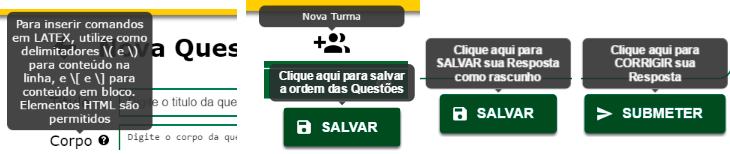
\includegraphics[width=0.9\textwidth]{prints/tooltip.png}
  \caption{Bolões com informações a respeito de sua função.}
  \label{print:tooltip}
  \vspace{-0.5cm}
\end{figure}

  Então podemos concluir que o designer do DFAjudge consegue ser muito satisfatório a respeito da navegação entre as páginas e da usabilidade de suas funcionalidades. O sistema apresenta todos os elementos de forma consistente, ou seja, todos os botões tem aparência semelhante e estão sempre ao final do formulário, os links utilizam imagens para simbolizar sua ação, e todos os outros elementos que constituem as páginas mantêm sempre a mesma aparência, tando das cores, quanto das suas localizações. Para que assim tenhamos maior clareza na utilização das interfaces deste sistema. 


% \clearpage
%  \noindent - clareza = Para uma interface ser eficaz e eficiente, o usuário deve ser capaz de reconhecer a sua utilidade e entender como ela pode ajudá-lo, prever o que vai acontecer durante o uso, e conseguir interagir com sucesso\\
%  - user no controle\\
%  - manipula diretamente o obj\\
%  - Um objetivo principal por tela\\
%  - consistência = botoes iguais, link sempre como img, linha clicável,\\
%  - simplicidade\\
%  - cor \\
%  - revelação progressiva\\
%  - ajudar o user no contexto = baloes com descrição.\\


%  \clearpage
%  \noindent TELAS Interface final:\\
%    - login, recuperar, def senha\\
%    - Emails\\
%    - Home\\
%    - Menu\\
%    visao prof\\
%    visao aluno\\
%    opcoes, ajuda, sobre, sair\\

%  \noindent Conceito estético (Designer + função)\\
%    cores\\
%    logos\\
%    Menu\\
%    Toolbar (voltar, titulo, acao)\\
%    listagem\\
%    botao de conclusao ( inserir, salvar, submeter)\\
%    Info localizado sempre no msm lugar = concisão\\
%    nao responsivo\\
%    acessibilidade? (todos clicaveis tem descricao)\\
 



\chapter[Teste do sistema em uma turma]{Teste do sistema em uma turma}
  
  Ao final do desenvolvimento deste sistema, houve a oportunidade de utiliza-lo, em caráter experimental, em duas turmas ofertadas da disciplina de Linguagens Formais e Autômatos no segundo quadrimestre de 2016. Então, neste capítulo relataremos os resultados obtidos.

  %Durante todo o desenvolvimento e deste teste do DFAjudge, foi utilizado um servidor comercial adquirido pelo orientador, na qual não foi possível utilizar o padrão HTTPS\footnote{Abreviação de \textit{Hyper Text Transfer Protocol Secure}, em português, Protocolo de Transferência de Hipertexto Seguro, é uma implementação do protocolo HTTP sobre uma camada adicional de segurança.}, mas isto não prejudicou em nada o funcionamento do sistema.

  O sistema foi apresentado às turmas pelo professor da disciplina, que é o orientador deste projeto, na primeira semana de aula. Então, seguindo o plano de ensino, após as aulas introdutórias sobre autômato finito determinístico (AFD), os alunos foram adicionados ao sistema. A estas turmas foi aplicada a primeira lista com questões básicas, afim de que os alunos pudessem treinar os conceitos fundamentais de AFD.
  
  Nas semanas seguintes, outras listas foram aplicadas, que abrangiam questões mais complexas do que as primeiras, como divisibilidade e aritmética em autômatos finitos determinísticos. No total, foram aplicadas 4 listas a estas turmas, cada uma delas com 10 questões, totalizando 40 questões que abrangem os tópicos relativos a AFD na disciplina de Linguagens Formais e Autômatos.

  Como o sistema estava sendo utilizado caráter experimental nas duas turmas, o professor não considerou obrigatório o uso do sistema e somente 40\% dos alunos o utilizaram pelo menos uma vez. Destes, uma fração menor ainda resolveu de fato as listas, como podemos ver no gráfico a seguir, o histograma das notas obtidas no relatório de desempenho das duas turmas unidas.

\begin{figure}[H]
  \centering
  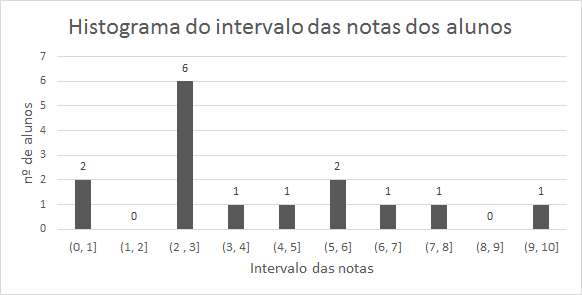
\includegraphics[scale=0.8]{histNotas.png}
  \caption{Histograma das notas que os alunos obtiveram.}
  \label{print:histNotas}
  %\vspace{-0.5cm}
\end{figure}  
  
  Afim de analisar o impacto da utilização do sistema no desempenho dos alunos, calculamos o coeficiente de correlação entre a proporção de exercícios resolvidos e a nota dos alunos. O coeficiente de correlação indica o quanto duas variáveis estão relacionadas entre si, e será sempre um valor entre $-$1 e 1. Quanto mais próximo de 1, mais fortemente e positivamente correlacionados os dois dados estão; quanto mais próximo de $-$1 mais inversamente correlacionados eles estão; e se o coeficiente de correlação estiver próximo de 0, não há correlação entre os dados. Para as turmas ministradas no segundo quadrimestre de 2016, calculamos o coeficiente de correlação entre o percentual de uso do sistema e: a nota da P1, a nota da P2 e a média das provas. 
  
% Correlação:\\
% P1 = 0,443637036\\
% P2 = 0,487210236\\
% MP = 0,575053945\\
\begin{table}[H]
  \centering
  \begin{tabular}{l|c} %\hline 
                                       & Correlação \\ \hline 
    Porcentagem de uso do sistema e P1 & 0,443637036 \\ %\hline 
    Porcentagem de uso do sistema e P2 & 0,487210236 \\ %\hline 
    Porcentagem de uso do sistema e MP & 0,575053945 \\ %\hline 
  \end{tabular} 
  \caption{Coeficiente de correlação entre a nota do sistema e das provas.}
  \vspace{-0.5cm}
\end{table}
  
  Podemos interpretar, considerando estes valores, que a utilização do sistema para a realização dos exercícios foi benéfica para a fixação dos conceitos, pois há uma clara relação positiva entre resolver as questões e a obter boa nota nas provas.

  Outro resultado importante para comentar, é que durante o uso intenso do sistema pelos alunos não houve nenhuma falha. %E agora com o banco de dados populado com questões que contemplam autômatos mais complexos, inúmeros pequenos teste eram executados afim de verificar a confiabilidade do sistema.
  
  %Estes testes se tratavam de submeter possíveis autômatos-respostas incorretos, utilizando a interface do aluno, afim de verificar a confiabilidade tanto do DFAdesigner, quanto do Juiz. Assim a cada submissão, o sistema atendia corretamente com o veredicto esperado. Demonstrando então o correto funcionamento do sistema em conjunto ao algoritmo de teste de equivalência de Hopcroft e Karp.
  
%  \noindent falar do pq nao usa HTTPS OK\\
%  usado na turma 2016q2 OK \\
%  Resultados obtidos (fez exercico -> acertou na prova) OK\\
 
 
 


\chapter[Próximos Passos]{Próximos Passos}%{Futuras Melhorias}

  Embora o sistema tenha sido criado para ser utilizado como uma plataforma de aplicação e correção automática de exercícios que tratam especificamente de autômatos finitos determinísticos, acreditamos que o nosso sistema poderia ser estendido para cobrir outros tipos de exercício envolvendo não só outros tópicos da disciplina de Linguagens Formais e Autômatos, mas também de qualquer outra disciplina, desde que o exercício admita um algoritmo de correção automática. Projetamos o sistema para atender somente uma classe de questões, mas do modo que estruturamos suas regras, seria possível, com poucas adaptações, servir também novas classes de exercícios, bastando somente seguir o mesmo modelo dos componentes implementados: ter um método para o aluno confeccionar sua resposta no \textit{front-end} e um juiz que implemente os devidos algoritmos para corrigir a resposta automaticamente no \textit{back-end}.

  Um ponto a ser melhorado no sistema está na listagem dos dados no gerenciamento de algumas entidades, como das listas e das questões pois, com o aumento quantidade de dados, cresce também a necessidade de apresentar os dados de maneira sucinta. O orientador sentiu alguma dificuldade na hora de criar uma lista, pois todas as questões que ele havia introduzido no sistema aparecem de uma vez, em sequência, e ele reportou que fica difícil procurar as questões que deseja. Isso poderia ser melhorado com o auxilio de filtros e ordenações dinâmicas do conteúdo, o que facilitaria a gestão destas entidades. % bastante

  O DFAdesigner é uma especialização do FSM, mas também poderia ser aprimorado adicionando-se elementos extras, tais como: permitir a definição de um estado como sendo um de morte -- estados que não são de aceitação em que todas as transições vão para o próprio estado, porém sem a necessidade de explicitar as transições uma a uma no designer -- abranger outros tipos de autômatos, ter uma área de trabalho dinâmica, ou seja, o espaço reservado para a confecção do AFD poderia ser redimensionável no próprio navegador.

  Uma das ideias que tivemos no início do desenvolvimento do sistema era permitir que os usuários do tipo professor pudessem compartilhar as questões uns com os outros por meio de um banco público de questões, mas isto aumentaria a complexidade das regras internas do sistema e assim tomamos a decisão de não implementar esta funcionalidade.

  Outra ideia interessante era de tornar o sistema público, ou seja, aberto para qualquer usuário que quisesse se cadastrar, permitindo que ele o utilizasse para responder questões e também criar novas questões. Deste modo, o sistema não seria segmentado em turmas de alunos de um professor, mas os usuários teriam papéis similares e poderiam também ter seus desempenhos ranqueados para que pudessem se comparar com os outros usuários.
  
  %Este sistema se tornou uma iniciativa para outros projetos que buscam criar um sistema que auxilie na aprendizagem, pois facilmente poderia dar continuidade a este projeto afim de abranger outras áreas.


 
%  \noindent CAPITULO: FUTURAS MELHORIAS e PROJETOS FUTUROS\\
%  add mais tipos de questões (Questões eh genérico) OK\\
%  aberto ao publico para resolver (ex: URI) OK\\
%  questões publicas entre professores OK\\
%  melhorar o gerenciamento ( add busca/filtro e pagina na listagem ) OK\\
%  melhorar o DFAdesigner OK\\

%\clearpage
%\noindent 
%  - código do sistema no github (DFAjudge e do DFAdesigner)\\
%  - login para o quem for ler o relatório, para testar online\\
%  apêndice de questões\\
%  licencaMIT\\
%  projetos futuros (continuação)\\


%  \noindent TODO:\\
%  - otimizacao do MOORE REMOVIDO\\
%  - AUT do canvas do Evan na pag 21 (transicao errada) OK\\
%  - add mais exemplos FICA PRA PROXIMA\\
%  - descrever o processo a partir do Lema 1 OK revisar OK\\


% ---
% Conclusão
% ---

\chapter[Conclusão]{Conclusão}

  Desenvolver o DFAjudge foi um desafio, mas ajudou a melhorar minhas práticas de programação e organização no desenvolvimento de um sistema web. Estudar a fundo os conceitos algorítmicos necessários para sua implementação (que antes eu somente tinha visto em sala de aula) e coloca-los em prática, para resolver problemas reais, foram de grande valia. Para o aluno, ter seus exercícios corrigidos instantaneamente é, de fato, muito útil para ajuda-lo a corrigir as falhas do aprendizado e para fixar os conceitos apresentados em aula, e isso foi demonstrado nas primeiras turmas que utilizaram este sistema. Com o DFAjudge concluído, os próximos passos seriam abranger sua atuação para outras áreas, onde a correção instantânea de execícios sejam de grande importância, a começar pelos autômatos finitos não determinísticos e pelos demais tópicos da disciplina de Linguagens Formais e Autômatos. 
  
  
  %Desenvolver o DFAjudge foi um desafio, mas ajudou a melhorar minhas práticas no desenvolvimento de um sistema web. Estudar a fundo conceitos, antes somente vistos em aula, e coloca-los em prática, para resolver problemas reais, foram de grande valia. Para o aluno, ter seus exercícios corrigidos instantaneamente é, de fato, muito útil para ajuda-lo a fixar os conceitos apresentados em aula, e isso foi demonstrado nas primeiras turmas que utilizaram este sistema. Com o DFAjudge concluído, os próximos passos será abranger sua atuação para outras áreas, onde a correção instantânea de execícios sejam de grande importância. % e outros projetos futuros.



% ----------------------------------------------------------
% ELEMENTOS PÓS-TEXTUAIS
% ----------------------------------------------------------
%\postextual
% ----------------------------------------------------------

% ----------------------------------------------------------
% Referências bibliográficas
% ----------------------------------------------------------
\bibliography{RelFinal}

% ----------------------------------------------------------
% Glossário
% ----------------------------------------------------------
%
% Consulte o manual da classe abntex2 para orientações sobre o glossário.
%
%\glossary

% ----------------------------------------------------------
% Apêndices
% ----------------------------------------------------------

% ---
% Inicia os apêndices
% ---
%\begin{apendicesenv}
%
%% Imprime uma página indicando o início dos apêndices
%\partapendices
%
%% ----------------------------------------------------------
%\chapter{Quisque libero justo}
%% ----------------------------------------------------------
%
%\lipsum[50]
%
%% ----------------------------------------------------------
%\chapter{Nullam elementum urna vel imperdiet sodales elit ipsum pharetra ligula
%ac pretium ante justo a nulla curabitur tristique arcu eu metus}
%% ----------------------------------------------------------
%\lipsum[55-57]
%
%\end{apendicesenv}
% ---


% ----------------------------------------------------------
% Anexos
% ----------------------------------------------------------

% ---
% Inicia os anexos
% ---
%\begin{anexosenv}
%
%% Imprime uma página indicando o início dos anexos
%\partanexos
%
%% ---
%\chapter{Morbi ultrices rutrum lorem.}
%% ---
%\lipsum[30]
%
%% ---
%\chapter{Cras non urna sed feugiat cum sociis natoque penatibus et magnis dis
%parturient montes nascetur ridiculus mus}
%% ---
%
%\lipsum[31]
%
%% ---
%\chapter{Fusce facilisis lacinia dui}
%% ---
%
%\lipsum[32]
%
%\end{anexosenv}

%---------------------------------------------------------------------
% INDICE REMISSIVO
%---------------------------------------------------------------------
%\phantompart
%\printindex
%---------------------------------------------------------------------

\end{document}
